\documentclass[12pt]{article}\usepackage[]{graphicx}\usepackage[]{color}
%% maxwidth is the original width if it is less than linewidth
%% otherwise use linewidth (to make sure the graphics do not exceed the margin)
\makeatletter
\def\maxwidth{ %
  \ifdim\Gin@nat@width>\linewidth
    \linewidth
  \else
    \Gin@nat@width
  \fi
}
\makeatother

\definecolor{fgcolor}{rgb}{0.345, 0.345, 0.345}
\newcommand{\hlnum}[1]{\textcolor[rgb]{0.686,0.059,0.569}{#1}}%
\newcommand{\hlstr}[1]{\textcolor[rgb]{0.192,0.494,0.8}{#1}}%
\newcommand{\hlcom}[1]{\textcolor[rgb]{0.678,0.584,0.686}{\textit{#1}}}%
\newcommand{\hlopt}[1]{\textcolor[rgb]{0,0,0}{#1}}%
\newcommand{\hlstd}[1]{\textcolor[rgb]{0.345,0.345,0.345}{#1}}%
\newcommand{\hlkwa}[1]{\textcolor[rgb]{0.161,0.373,0.58}{\textbf{#1}}}%
\newcommand{\hlkwb}[1]{\textcolor[rgb]{0.69,0.353,0.396}{#1}}%
\newcommand{\hlkwc}[1]{\textcolor[rgb]{0.333,0.667,0.333}{#1}}%
\newcommand{\hlkwd}[1]{\textcolor[rgb]{0.737,0.353,0.396}{\textbf{#1}}}%

\usepackage{framed}
\makeatletter
\newenvironment{kframe}{%
 \def\at@end@of@kframe{}%
 \ifinner\ifhmode%
  \def\at@end@of@kframe{\end{minipage}}%
  \begin{minipage}{\columnwidth}%
 \fi\fi%
 \def\FrameCommand##1{\hskip\@totalleftmargin \hskip-\fboxsep
 \colorbox{shadecolor}{##1}\hskip-\fboxsep
     % There is no \\@totalrightmargin, so:
     \hskip-\linewidth \hskip-\@totalleftmargin \hskip\columnwidth}%
 \MakeFramed {\advance\hsize-\width
   \@totalleftmargin\z@ \linewidth\hsize
   \@setminipage}}%
 {\par\unskip\endMakeFramed%
 \at@end@of@kframe}
\makeatother

\definecolor{shadecolor}{rgb}{.97, .97, .97}
\definecolor{messagecolor}{rgb}{0, 0, 0}
\definecolor{warningcolor}{rgb}{1, 0, 1}
\definecolor{errorcolor}{rgb}{1, 0, 0}
\newenvironment{knitrout}{}{} % an empty environment to be redefined in TeX

\usepackage{alltt}
\usepackage[utf8]{inputenc}
\usepackage{graphicx}
\usepackage{color}
\definecolor{blue1}{RGB}{0,102,204}
\usepackage[colorlinks = true,linkcolor = blue,citecolor = blue,urlcolor = blue]{hyperref}
\usepackage{array}
\usepackage[english]{babel}
\usepackage{amsfonts}
\usepackage{url}
\usepackage{bm}
\usepackage[margin = 1.5cm]{geometry}
\usepackage[affil-it]{authblk}
\usepackage{hyperref}

\newcommand{\R}{\mathbb{R}}
\newcommand{\code}[1]{{{\tt #1}}}


\title{Illustrating package cati (Community Assembly by Traits: Individuals and beyond) using Darwin finches data}
\author{Adrien Taudiere\thanks{\texttt{adrien.taudiere@cefe.cnrs.fr}} and Cyrille Violle}

\affil{{\footnotesize CEFE - Centre d'Ecologie Fonctionnelle et Evolutive, Montpellier: France}}

\date{\today}

\sloppy
\hyphenpenalty 10000

%%%%%%%%%%%%%%%%%%%%%%%%%%%%%%%%%%%%%%%%%%%%%%%%%%
%%%%%%%%%%%%%%%%%%%%%%%%%%%%%%%%%%%%%%%%%%%%%%%%%%
%%%%%%%%%%%%%%%%%%%%%%%%%%%%%%%%%%%%%%%%%%%%%%%%%%
\IfFileExists{upquote.sty}{\usepackage{upquote}}{}
\begin{document}

\selectlanguage{english}



\maketitle


\textbf{Abstract:}

\textbf{Key words:}
Functional space, functional structure, community assembly, ecological niche, environmental filter, individual differences, intraspecific variation, null model, trait, variance decomposition

\vfill
\begin{center}
\textbf{The up to date version of this tutorial is available \href{http://sourceforge.net/p/cati-r/code/ci/master/tree/tutorial/vignettes/vignette.pdf}{here}.}
\end{center}

\newpage
\tableofcontents

\newpage


\section{Introduction}
This vignette present the \texttt{cati} package for R (Community Assembly by Traits: Individuals and beyond) using Darwin finches data.

\section{Getting started}
\subsection{Installing the package \texttt{cati}}

Before going further, we shall make sure that \texttt{cati} is well installed
on the computer.
The current version of the package is 0.94.
Make sure you have a recent version of R ($\geq 3.0.2$) by typing:

\begin{knitrout}
\definecolor{shadecolor}{rgb}{0.969, 0.969, 0.969}\color{fgcolor}\begin{kframe}
\begin{alltt}
\hlstd{R.version.string}
\end{alltt}
\begin{verbatim}
## [1] "R version 3.1.2 (2014-10-31)"
\end{verbatim}
\end{kframe}
\end{knitrout}

Then, install \texttt{cati} with dependencies using:
\begin{knitrout}
\definecolor{shadecolor}{rgb}{0.969, 0.969, 0.969}\color{fgcolor}\begin{kframe}
\begin{alltt}
\hlcom{#install.packages("cati", repos = "http://cran.us.r-project.org", dependencies = TRUE)}
\hlkwd{library}\hlstd{(}\hlstr{"cati"}\hlstd{)}
\end{alltt}


{\ttfamily\noindent\itshape\color{messagecolor}{\#\# Loading required package: nlme\\\#\# Loading required package: ade4\\\#\# Loading required package: ape}}\end{kframe}
\end{knitrout}

We can now load the package alongside other useful packages:
\begin{knitrout}
\definecolor{shadecolor}{rgb}{0.969, 0.969, 0.969}\color{fgcolor}\begin{kframe}
\begin{alltt}
\hlkwd{library}\hlstd{(}\hlstr{"mice"}\hlstd{)}
\end{alltt}


{\ttfamily\noindent\itshape\color{messagecolor}{\#\# Loading required package: Rcpp\\\#\# Loading required package: lattice\\\#\# mice 2.22 2014-06-10}}\begin{alltt}
\hlkwd{library}\hlstd{(}\hlstr{"hypervolume"}\hlstd{)}
\end{alltt}


{\ttfamily\noindent\itshape\color{messagecolor}{\#\# Loading required package: rgl}}\end{kframe}
\end{knitrout}

You can make sure that the right version of the package is installed using:
\begin{knitrout}
\definecolor{shadecolor}{rgb}{0.969, 0.969, 0.969}\color{fgcolor}\begin{kframe}
\begin{alltt}
\hlkwd{packageDescription}\hlstd{(}\hlstr{"cati"}\hlstd{,} \hlkwc{fields} \hlstd{=} \hlstr{"Version"}\hlstd{)}
\end{alltt}
\begin{verbatim}
## [1] "0.94"
\end{verbatim}
\end{kframe}
\end{knitrout}
\texttt{cati} version should read 0.94.

\subsection{Getting help}

To get help for a given function, use \texttt{?foo} where \texttt{foo} is the
function of interest.
For instance:

\begin{knitrout}
\definecolor{shadecolor}{rgb}{0.969, 0.969, 0.969}\color{fgcolor}\begin{kframe}
\begin{alltt}
\hlopt{?}\hlstd{Tstats}
\end{alltt}
\end{kframe}
\end{knitrout}

will open up the manpage of T-statistics function (\texttt{Tstats}).
An 'example' section will shows how to use a function at the end of the manpage. 

Note that you can also browse help pages as html pages, using:
\begin{knitrout}
\definecolor{shadecolor}{rgb}{0.969, 0.969, 0.969}\color{fgcolor}\begin{kframe}
\begin{alltt}
\hlkwd{help.start}\hlstd{()}
\end{alltt}
\end{kframe}
\end{knitrout}

To go to the \texttt{cati} man page on Rstudio, click 'packages' in the lower right windows, then clik 'cati', and 'cati-package'.

\subsection{Data presentation: Darwin finches in Galapagos Island}

First we need to load the data.
\begin{knitrout}
\definecolor{shadecolor}{rgb}{0.969, 0.969, 0.969}\color{fgcolor}\begin{kframe}
\begin{alltt}
\hlkwd{data}\hlstd{(finch.ind)}

\hlcom{#Save default parameters}
\hlstd{old.par}\hlkwb{<-}\hlkwd{par}\hlstd{(}\hlkwc{no.readonly} \hlstd{=} \hlnum{TRUE}\hlstd{)}
\end{alltt}
\end{kframe}
\end{knitrout}

Now we can see 3 objects: a traits matrix \texttt{traits.finch}, a vector of species names \texttt{sp.finch} and a vector of sites names \texttt{ind.plot}. 
\begin{knitrout}
\definecolor{shadecolor}{rgb}{0.969, 0.969, 0.969}\color{fgcolor}\begin{kframe}
\begin{alltt}
\hlkwd{dim}\hlstd{(traits.finch)}
\hlcom{#the trait matrix contains 2513 individuals values for 4 traits}
\hlkwd{table}\hlstd{(sp.finch)}
\hlcom{#the species names vector contains 2513 individuals belonging to 12 species}
\hlkwd{table}\hlstd{(ind.plot.finch)}
\hlcom{#the sites names vector contains 2513 individuals belonging to 6 sites (Islands)}
\end{alltt}
\end{kframe}
\end{knitrout}

The four traits correspond to three beak traits and one wing trait.

\begin{center}
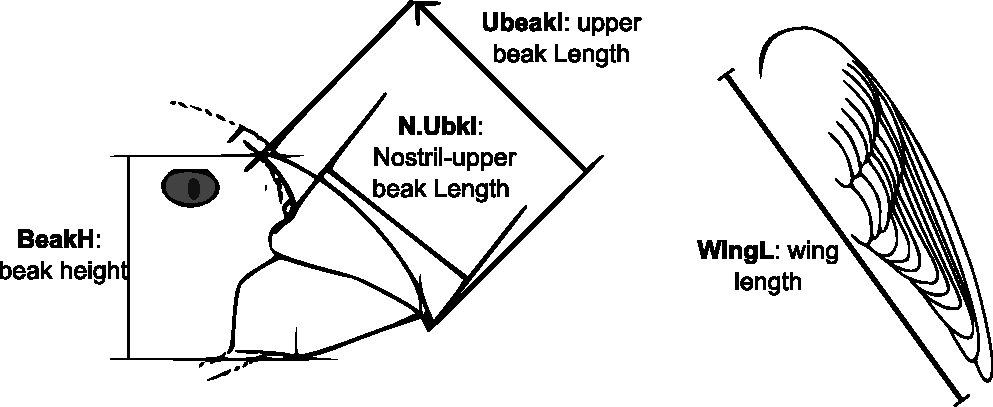
\includegraphics[width = 10cm]{figs/darwinfinch.pdf}
\end{center}

\newpage


%%%%%%%%%%%%%%%%
\section{Description of traits distributions}
%%%%%%%%%%%%%%%%

\subsection{Plot the kernel density of traits}

Plot the distribution of traits values for populations, species, sites and regional scales. First, let try the distribution for all populations of Darwin finches. In R, FALSE and TRUE can be written respectively \texttt{F} and \texttt{T}.

\begin{knitrout}
\definecolor{shadecolor}{rgb}{0.969, 0.969, 0.969}\color{fgcolor}\begin{kframe}
\begin{alltt}
\hlkwd{par}\hlstd{(}\hlkwc{mfrow} \hlstd{=} \hlkwd{c}\hlstd{(}\hlnum{4}\hlstd{,}\hlnum{4}\hlstd{),} \hlkwc{cex} \hlstd{=} \hlnum{0.5}\hlstd{)}
\hlkwd{plotDistri}\hlstd{(traits.finch, sp.finch, ind.plot.finch,}
           \hlkwc{ylim.cex} \hlstd{=} \hlnum{3}\hlstd{,} \hlkwc{plot.ask} \hlstd{= F,} \hlkwc{multipanel} \hlstd{= F,} \hlkwc{leg} \hlstd{= F)}
\end{alltt}
\end{kframe}
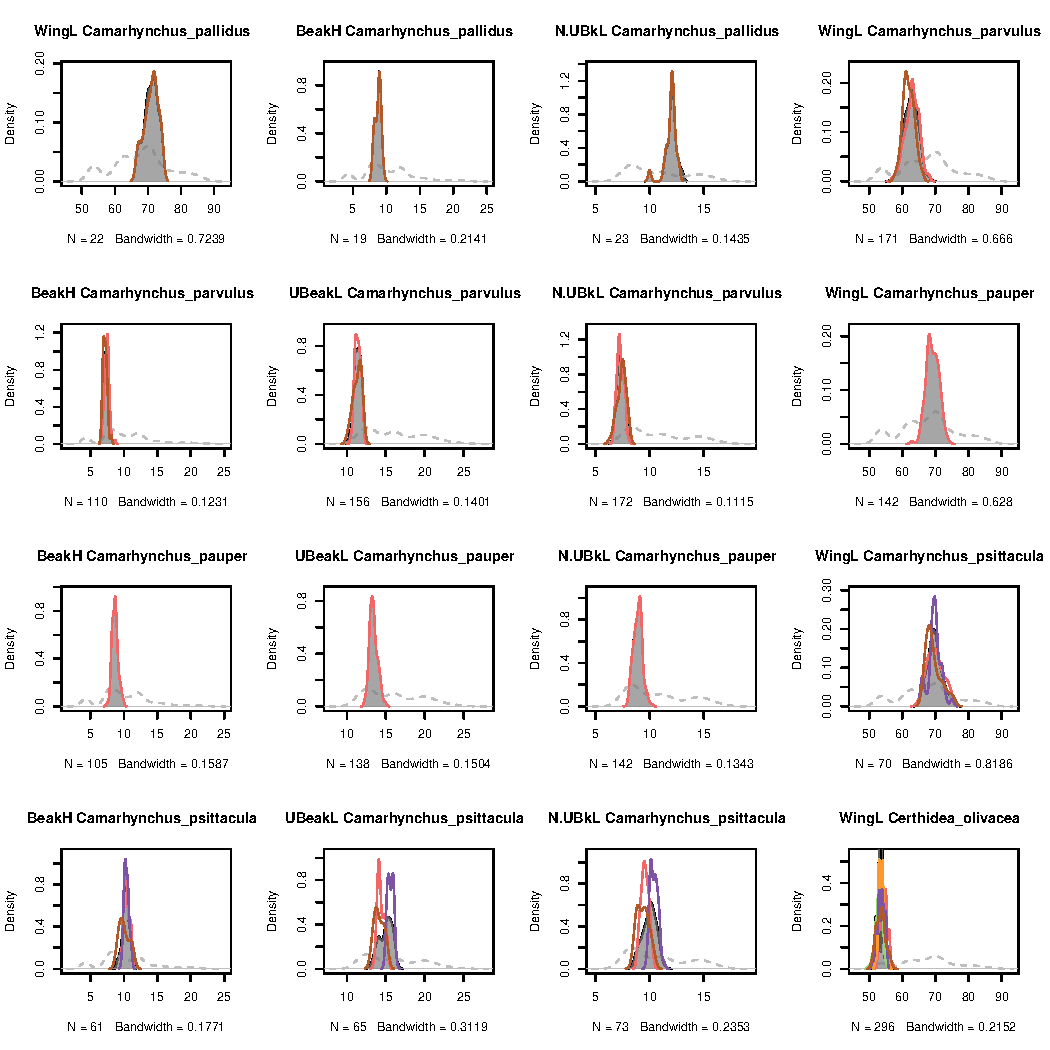
\includegraphics[width=\maxwidth]{figure/unnamed-chunk-10-1} 

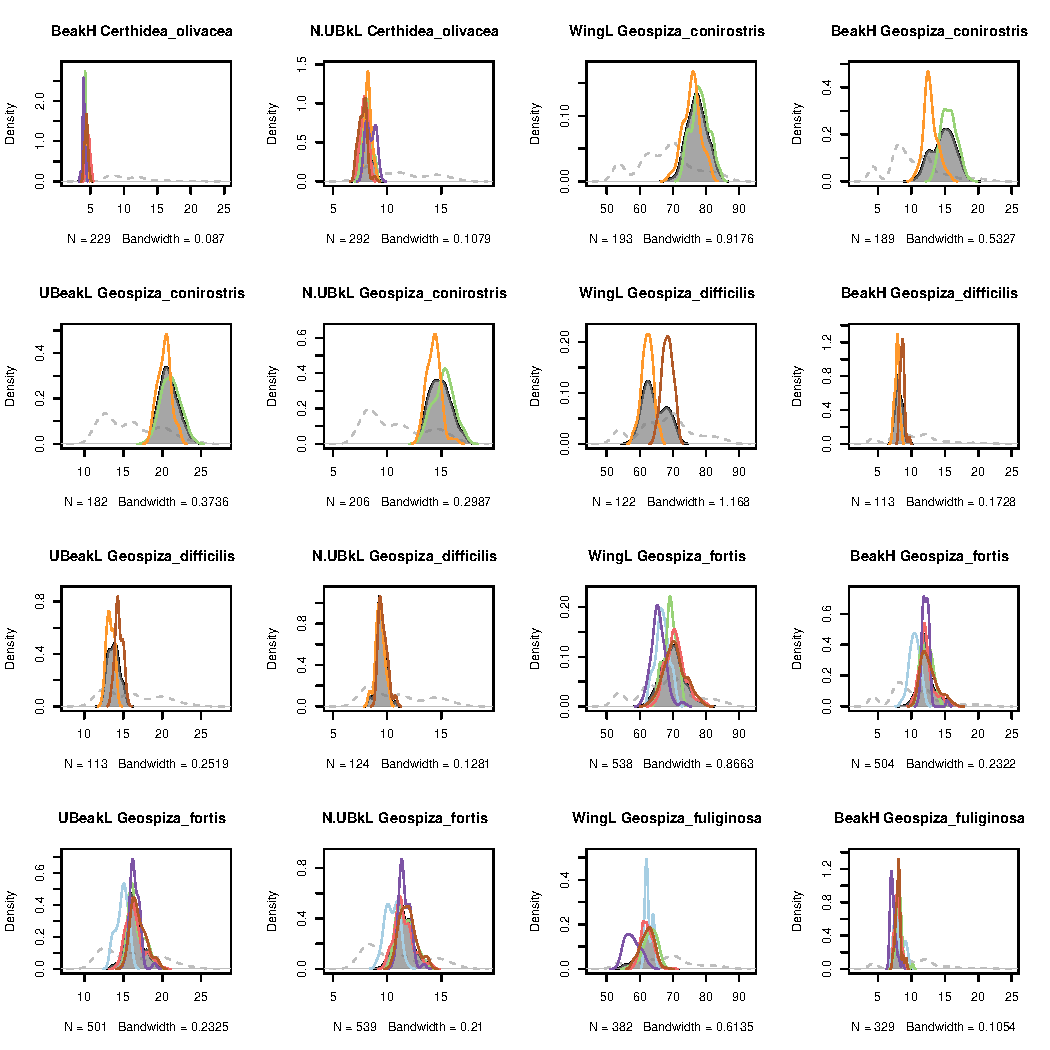
\includegraphics[width=\maxwidth]{figure/unnamed-chunk-10-2} 

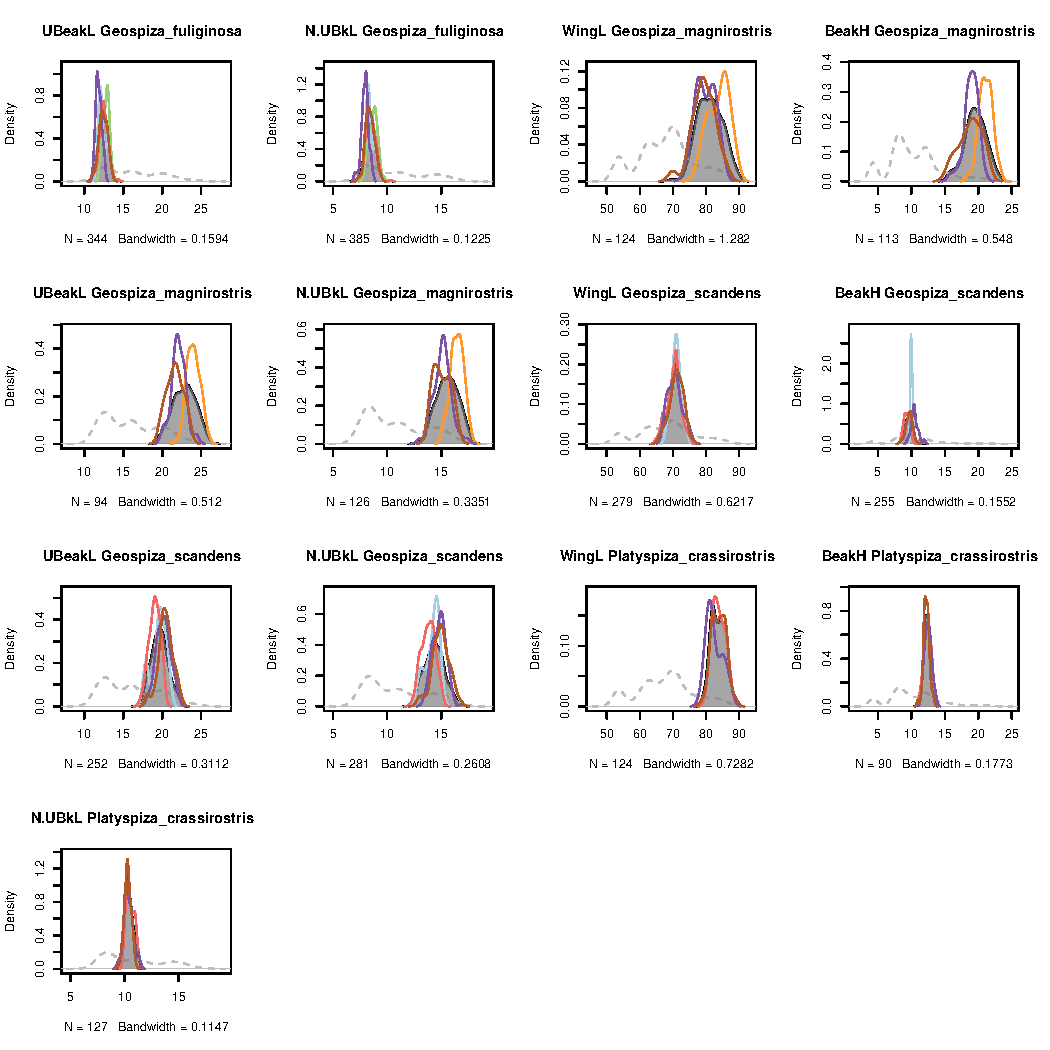
\includegraphics[width=\maxwidth]{figure/unnamed-chunk-10-3} 

\end{knitrout}
The argument \texttt{ylim.cex} define the magnification to be used for range of y axe. To understand the other argument, type \texttt{?plotDistri}.

\newpage

Then we can inverse the second and the third arguments to plot the distribution for all finches species. 

\begin{knitrout}
\definecolor{shadecolor}{rgb}{0.969, 0.969, 0.969}\color{fgcolor}\begin{kframe}
\begin{alltt}
\hlkwd{par}\hlstd{(}\hlkwc{mfrow} \hlstd{=} \hlkwd{c}\hlstd{(}\hlnum{4}\hlstd{,}\hlnum{4}\hlstd{),} \hlkwc{cex} \hlstd{=} \hlnum{0.5}\hlstd{)}
\hlkwd{plotDistri}\hlstd{(traits.finch, ind.plot.finch, sp.finch,}
           \hlkwc{ylim.cex} \hlstd{=} \hlnum{8}\hlstd{,} \hlkwc{plot.ask} \hlstd{= F,} \hlkwc{multipanel} \hlstd{= F,} \hlkwc{leg} \hlstd{= F)}
\end{alltt}
\end{kframe}
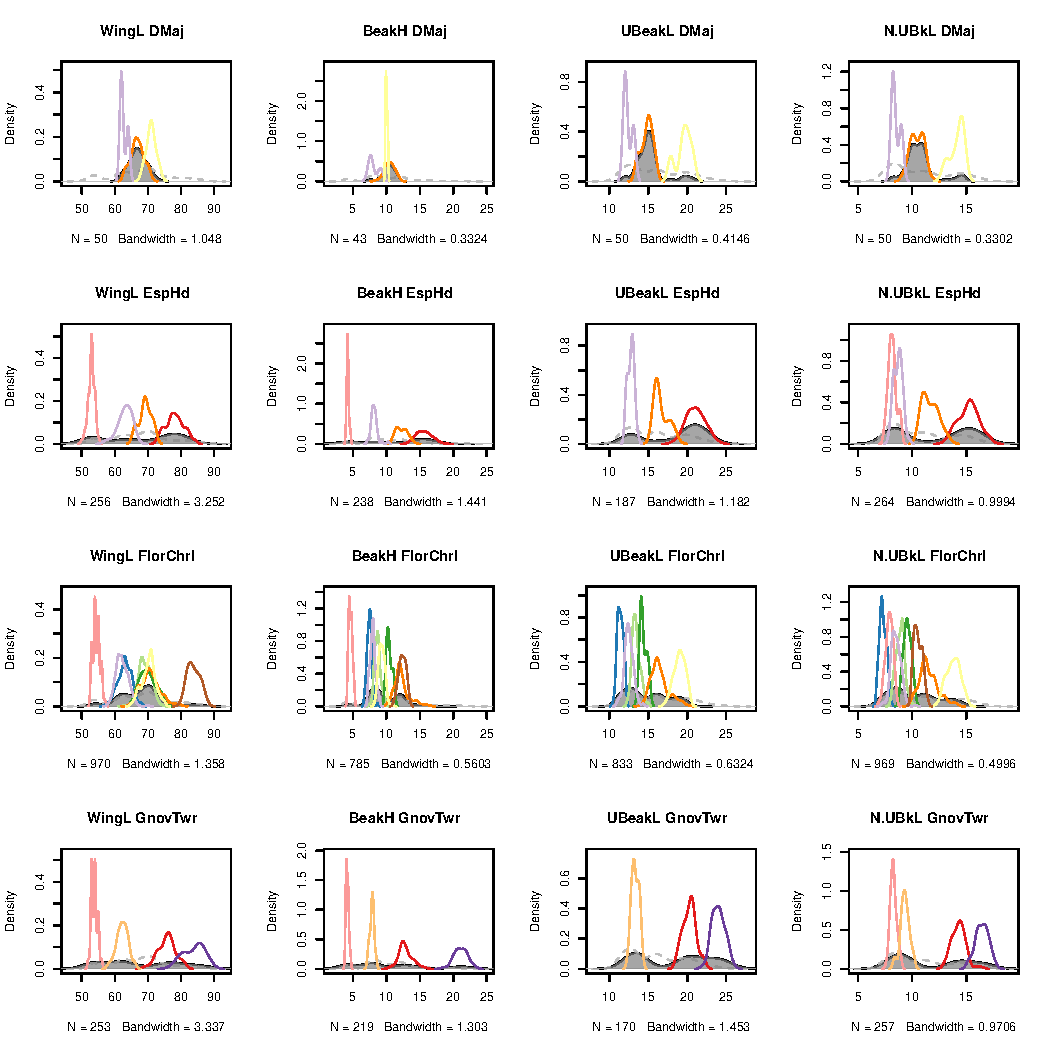
\includegraphics[width=\maxwidth]{figure/unnamed-chunk-11-1} 

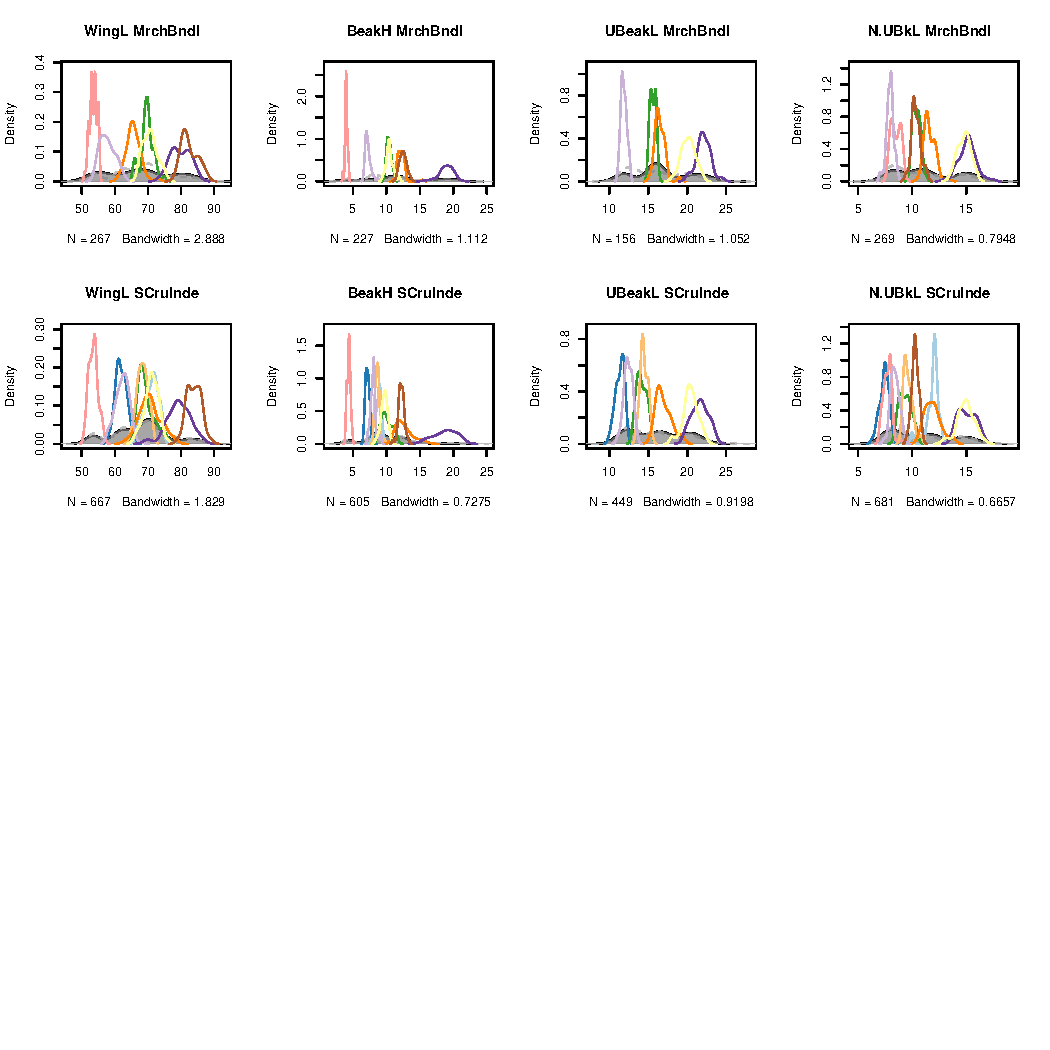
\includegraphics[width=\maxwidth]{figure/unnamed-chunk-11-2} 

\end{knitrout}

Now, see the result for only one trait with the legend (\texttt{leg = TRUE}). \texttt{cex.leg} specify the magnification of legend. 

\begin{knitrout}
\definecolor{shadecolor}{rgb}{0.969, 0.969, 0.969}\color{fgcolor}\begin{kframe}
\begin{alltt}
\hlkwd{par}\hlstd{(}\hlkwc{mfrow} \hlstd{=} \hlkwd{c}\hlstd{(}\hlnum{2}\hlstd{,}\hlnum{3}\hlstd{))}
\hlkwd{plotDistri}\hlstd{(}\hlkwd{as.matrix}\hlstd{(traits.finch[,}\hlnum{1}\hlstd{]), ind.plot.finch, sp.finch,}
          \hlkwc{ylim.cex} \hlstd{=} \hlnum{8}\hlstd{,} \hlkwc{plot.ask} \hlstd{= F,} \hlkwc{multipanel} \hlstd{= F,} \hlkwc{leg} \hlstd{= T,} \hlkwc{cex.leg} \hlstd{=} \hlnum{0.5}\hlstd{)}
\end{alltt}
\end{kframe}
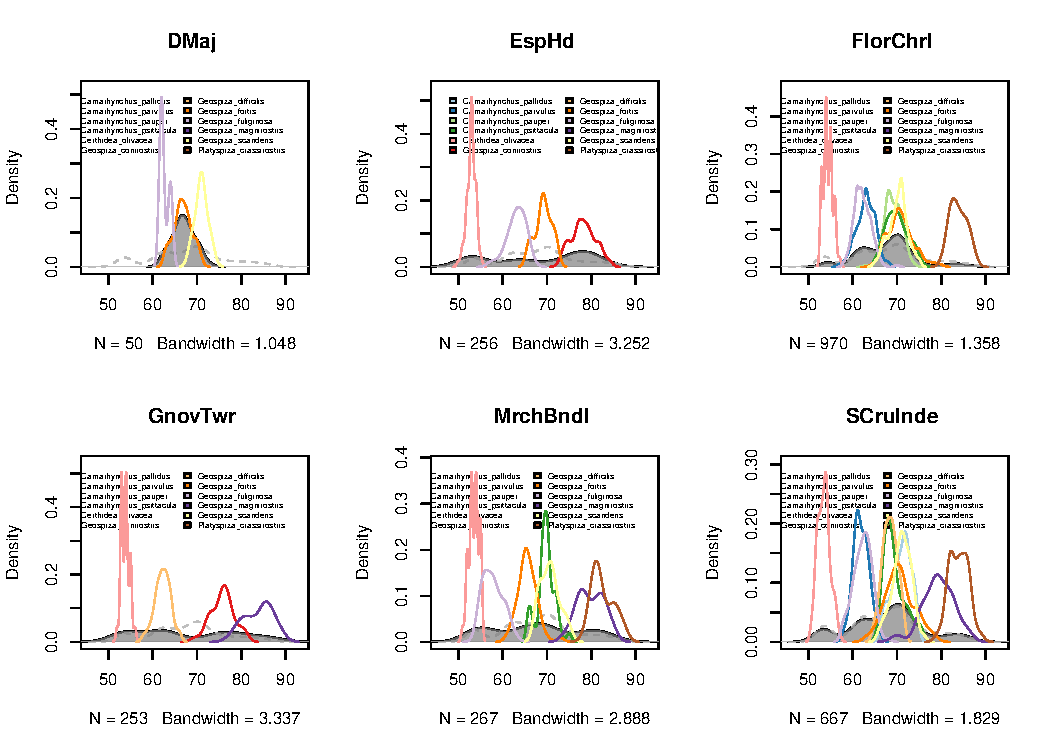
\includegraphics[width=\maxwidth]{figure/unnamed-chunk-12-1} 

\end{knitrout}

If we want to plot all the sites (regional distribution) or all the species: we can use the following code:
\begin{knitrout}
\definecolor{shadecolor}{rgb}{0.969, 0.969, 0.969}\color{fgcolor}\begin{kframe}
\begin{alltt}
\hlkwd{par}\hlstd{(}\hlkwc{mfrow} \hlstd{=} \hlkwd{c}\hlstd{(}\hlnum{4}\hlstd{,}\hlnum{4}\hlstd{),} \hlkwc{cex} \hlstd{=} \hlnum{0.5}\hlstd{)}
\hlkwd{plotDistri}\hlstd{(traits.finch,} \hlkwd{rep}\hlstd{(}\hlstr{"region"}\hlstd{,} \hlkwc{times} \hlstd{=} \hlkwd{dim}\hlstd{(traits.finch)[}\hlnum{1}\hlstd{]),}
           \hlstd{sp.finch,} \hlkwc{ylim.cex} \hlstd{=} \hlnum{6}\hlstd{,} \hlkwc{plot.ask} \hlstd{= F,} \hlkwc{leg} \hlstd{= F)}
\end{alltt}
\end{kframe}
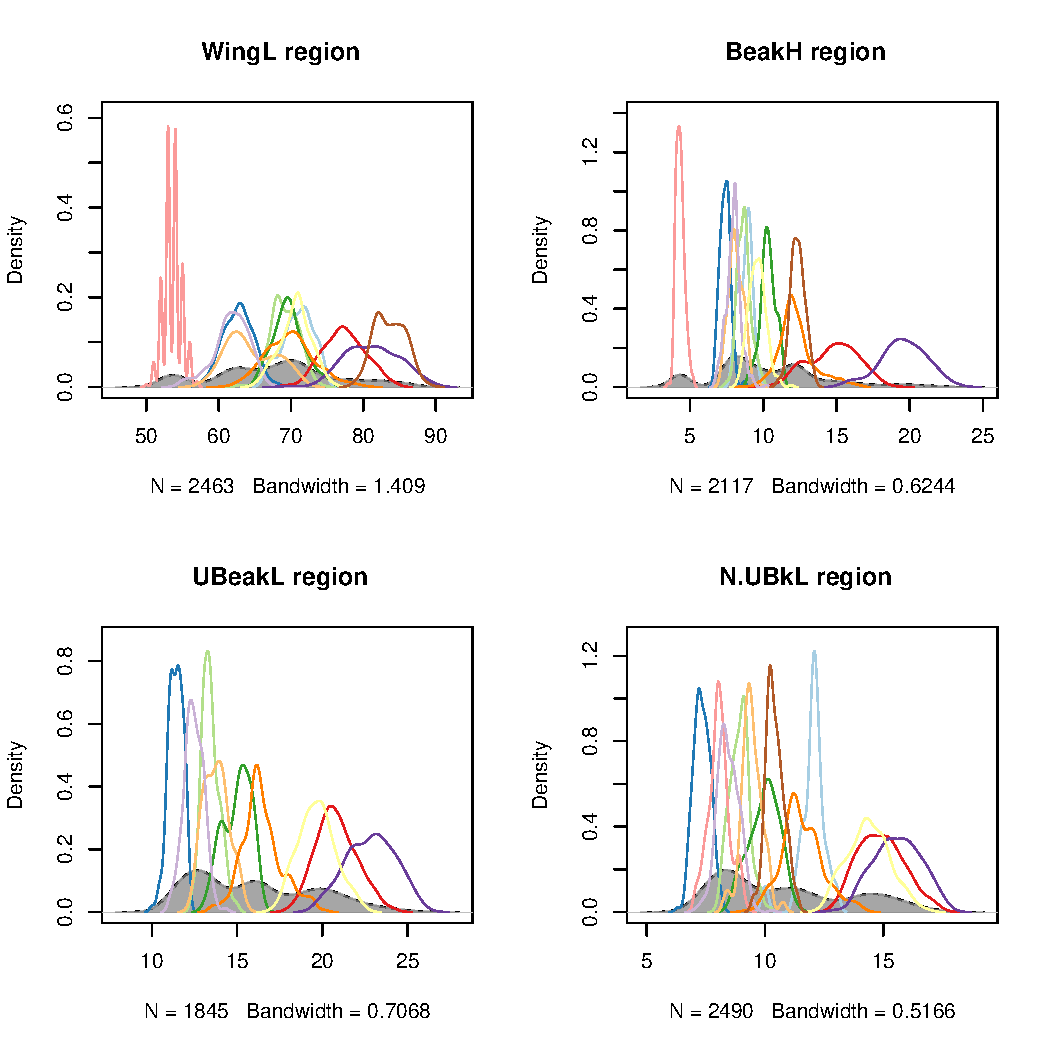
\includegraphics[width=\maxwidth]{figure/unnamed-chunk-13-1} 

\end{knitrout}

\begin{knitrout}
\definecolor{shadecolor}{rgb}{0.969, 0.969, 0.969}\color{fgcolor}\begin{kframe}
\begin{alltt}
\hlkwd{plotDistri}\hlstd{(traits.finch,} \hlkwd{rep}\hlstd{(}\hlstr{"all_sp"}\hlstd{,} \hlkwc{times} \hlstd{=} \hlkwd{dim}\hlstd{(traits.finch)[}\hlnum{1}\hlstd{]),}
           \hlstd{ind.plot.finch,} \hlkwc{ylim.cex} \hlstd{=} \hlnum{3}\hlstd{,} \hlkwc{plot.ask} \hlstd{= F,} \hlkwc{cex.leg} \hlstd{=} \hlnum{0.5}\hlstd{)}
\end{alltt}
\end{kframe}
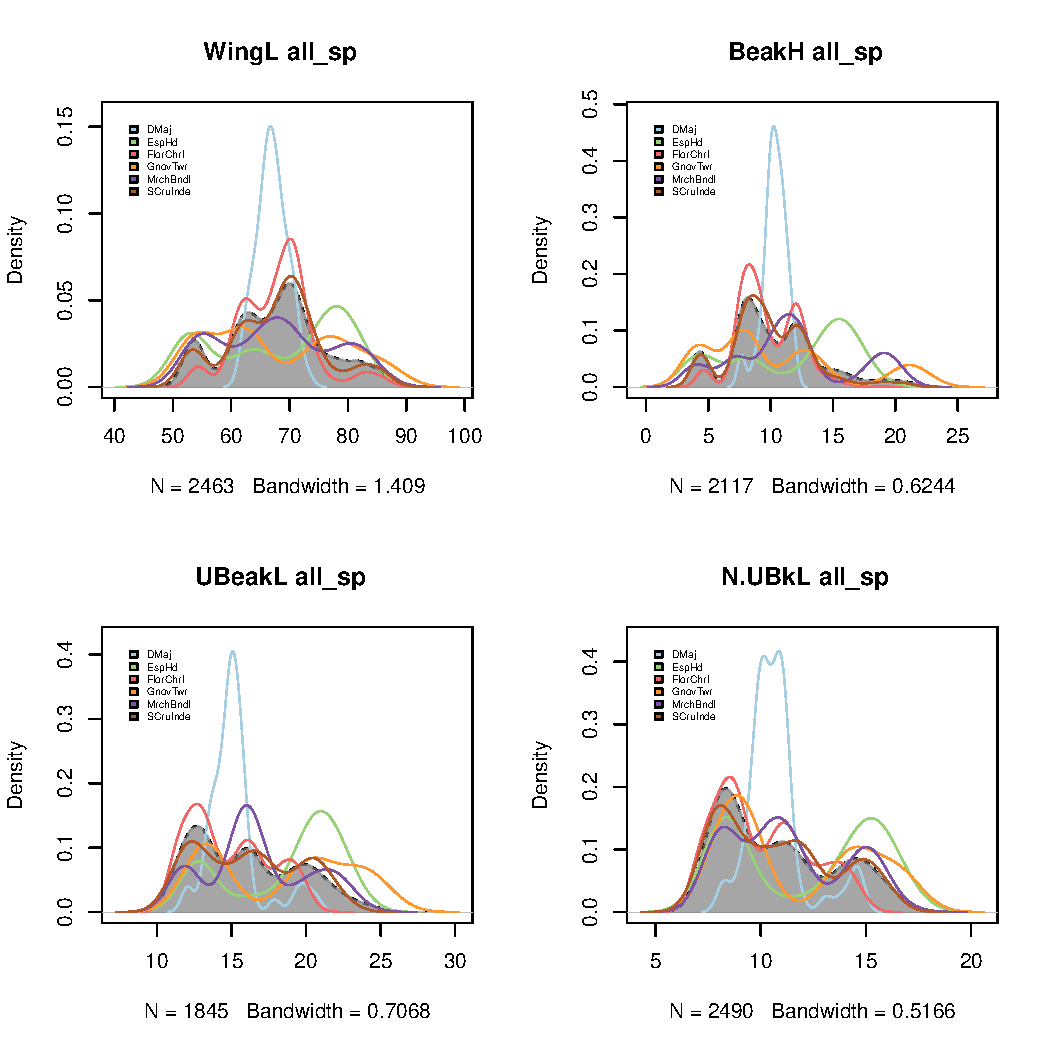
\includegraphics[width=\maxwidth]{figure/unnamed-chunk-14-1} 

\end{knitrout}

Now we can reset the default graphical parameter:
\begin{knitrout}
\definecolor{shadecolor}{rgb}{0.969, 0.969, 0.969}\color{fgcolor}\begin{kframe}
\begin{alltt}
\hlkwd{par}\hlstd{(old.par)}
\end{alltt}
\end{kframe}
\end{knitrout}
\newpage

%%%%%%%%%%%%%%%%
\section{Decomposition of variances}
%%%%%%%%%%%%%%%%

\subsection{Decomposition of within/among species variances using rao diversity}

The Rao function computes $\alpha$, $\beta$ and $\gamma$ -components for taxonomic, functional and/or phylogenetic diversity with:

$$ \gamma = mean (\alpha) + \beta $$

Where: $\gamma$ is the diversity of the regional pool, $\alpha$ is the diversity of the local community and $\beta$ is the turn over between local communities; diversity is estimated using the Rao quadratic entropy indices. Note that this method uses the additive framework of diversity. See the paper of Jost in 2010 (partitioning diversity into independent alpha and beta components) for more details on the differences between additive and multiplicative partitioning of diversity.


~\\

\textbf{Reference}: de Bello, F., Lavorel, S., Albert, C.H., Thuiller, W., Grigulis, K., Dolezal, J., Janecek, S. and Leps, J. (2011) Quantifying the relevance of intraspecific trait variability for functional diversity. Methods in Ecology and Evolution, 2, 163-174.


\subsubsection{Multitraits analysis}
First, rao diversity can be calculated on the functional  space (i.e. considering all traits together).

\begin{knitrout}
\definecolor{shadecolor}{rgb}{0.969, 0.969, 0.969}\color{fgcolor}\begin{kframe}
\begin{alltt}
\hlcom{#create individuals community matrix}
\hlstd{comm}\hlkwb{<-}\hlkwd{t}\hlstd{(}\hlkwd{table}\hlstd{(ind.plot.finch,}\hlnum{1}\hlopt{:}\hlkwd{length}\hlstd{(ind.plot.finch)))}
\hlcom{#create species community matrix}
\hlstd{comm.sp}\hlkwb{<-}\hlkwd{table}\hlstd{(sp.finch, ind.plot.finch)}
\hlkwd{class}\hlstd{(comm.sp)}\hlkwb{<-}\hlstr{"matrix"}
\hlstd{traits.finch.sp}\hlkwb{<-}\hlkwd{apply}\hlstd{(} \hlkwd{apply}\hlstd{(traits.finch,} \hlnum{2}\hlstd{, scale ),} \hlnum{2}\hlstd{,}
            \hlkwa{function}\hlstd{(}\hlkwc{x}\hlstd{)} \hlkwd{tapply}\hlstd{(x, sp.finch, mean,} \hlkwc{na.rm} \hlstd{= T))}
\hlstd{mat.dist}\hlkwb{<-}\hlkwd{as.matrix}\hlstd{(}\hlkwd{dist}\hlstd{(traits.finch.sp))}\hlopt{^}\hlnum{2}

\hlstd{ptm} \hlkwb{<-} \hlkwd{proc.time}\hlstd{()}

\hlstd{res.rao}\hlkwb{<-}\hlkwd{RaoRel}\hlstd{(}\hlkwc{sample} \hlstd{=} \hlkwd{as.matrix}\hlstd{(comm.sp),}
        \hlkwc{dfunc} \hlstd{= mat.dist,} \hlkwc{dphyl} \hlstd{=} \hlkwa{NULL}\hlstd{,}
        \hlkwc{weight} \hlstd{= F,} \hlkwc{Jost} \hlstd{= F,} \hlkwc{structure} \hlstd{=} \hlkwa{NULL}\hlstd{)}
\hlstd{proc.time_RaoRel} \hlkwb{<-} \hlkwd{proc.time}\hlstd{()} \hlopt{-} \hlstd{ptm}

\hlstd{witRao}\hlkwb{<-}\hlstd{res.rao}\hlopt{$}\hlstd{FD}\hlopt{$}\hlstd{Mean_Alpha} \hlcom{#overall within species variance}
\hlstd{betRao}\hlkwb{<-}\hlstd{res.rao}\hlopt{$}\hlstd{FD}\hlopt{$}\hlstd{Beta_add}  \hlcom{#between species variance}
\hlstd{totRao}\hlkwb{<-}\hlstd{res.rao}\hlopt{$}\hlstd{FD}\hlopt{$}\hlstd{Gamma}    \hlcom{#the total variance}

\hlcom{#Check that the total variance is equal}
\hlcom{#to between species + within species variances}
\hlstd{witRao}\hlopt{+}\hlstd{betRao}
\end{alltt}
\begin{verbatim}
## [1] 8.369581
\end{verbatim}
\begin{alltt}
\hlstd{totRao}
\end{alltt}
\begin{verbatim}
## [1] 8.369581
\end{verbatim}
\end{kframe}
\end{knitrout}

Now let's take the abundance into account to calculate Rao diversity.

\begin{knitrout}
\definecolor{shadecolor}{rgb}{0.969, 0.969, 0.969}\color{fgcolor}\begin{kframe}
\begin{alltt}
\hlstd{res.rao.w}\hlkwb{<-}\hlkwd{RaoRel}\hlstd{(}\hlkwc{sample} \hlstd{=} \hlkwd{as.matrix}\hlstd{(comm.sp),}
         \hlkwc{dfunc} \hlstd{= mat.dist,} \hlkwc{dphyl} \hlstd{=} \hlkwa{NULL}\hlstd{,}
         \hlkwc{weight} \hlstd{= T,} \hlkwc{Jost} \hlstd{= F,} \hlkwc{structure} \hlstd{=} \hlkwa{NULL}\hlstd{)}

\hlstd{witRao.w}\hlkwb{<-}\hlstd{res.rao.w}\hlopt{$}\hlstd{FD}\hlopt{$}\hlstd{Mean_Alpha} \hlcom{#overall within species variance}
\hlstd{betRao.w}\hlkwb{<-}\hlstd{res.rao.w}\hlopt{$}\hlstd{FD}\hlopt{$}\hlstd{Beta_add}  \hlcom{#between species variance}
\hlstd{totRao.w}\hlkwb{<-}\hlstd{res.rao.w}\hlopt{$}\hlstd{FD}\hlopt{$}\hlstd{Gamma}    \hlcom{#the total variance}

\hlstd{witRao.w}
\end{alltt}
\begin{verbatim}
## [1] 7.550591
\end{verbatim}
\begin{alltt}
\hlstd{betRao.w}
\end{alltt}
\begin{verbatim}
## [1] 0.3457724
\end{verbatim}
\end{kframe}
\end{knitrout}

Plot the results.

\begin{knitrout}
\definecolor{shadecolor}{rgb}{0.969, 0.969, 0.969}\color{fgcolor}\begin{kframe}
\begin{alltt}
\hlkwd{barplot}\hlstd{(}\hlkwd{cbind}\hlstd{(}\hlkwd{c}\hlstd{(witRao.w, betRao.w),} \hlkwd{c}\hlstd{(witRao, betRao)),}
    \hlkwc{names.arg} \hlstd{=} \hlkwd{c}\hlstd{(}\hlstr{"abundance"} \hlstd{,}\hlstr{"presence"}\hlstd{),}
    \hlkwc{legend.text} \hlstd{=} \hlkwd{c}\hlstd{(}\hlstr{"within species"}\hlstd{,} \hlstr{"between species"}\hlstd{),}
    \hlkwc{ylab} \hlstd{=} \hlstr{"Rao"}\hlstd{,} \hlkwc{ylim} \hlstd{=} \hlkwd{c}\hlstd{(}\hlnum{0}\hlstd{,}\hlnum{10}\hlstd{))}
\end{alltt}
\end{kframe}

{\centering 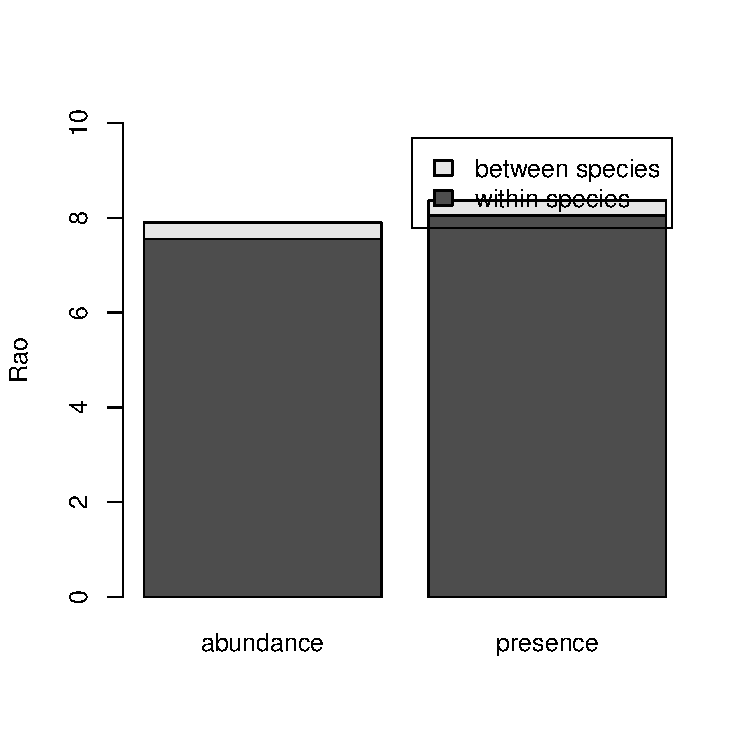
\includegraphics[width=\maxwidth]{figure/unnamed-chunk-18-1} 

}



\end{knitrout}


\subsubsection{Unitraits analysis}
We can also do this analysis for each trait separately. We need to replace (or exclude) NA values. For this example, we use the package \texttt{mice} to complete the data.

\begin{knitrout}
\definecolor{shadecolor}{rgb}{0.969, 0.969, 0.969}\color{fgcolor}\begin{kframe}
\begin{alltt}
\hlstd{comm}\hlkwb{<-}\hlkwd{t}\hlstd{(}\hlkwd{table}\hlstd{(ind.plot.finch,}\hlnum{1}\hlopt{:}\hlkwd{length}\hlstd{(ind.plot.finch)))}

\hlkwd{require}\hlstd{(mice)}
\hlstd{traits} \hlkwb{=} \hlstd{traits.finch}
\hlstd{mice}\hlkwb{<-}\hlkwd{mice}\hlstd{(traits.finch)}
\hlstd{traits.finch.mice}\hlkwb{<-}\hlkwd{complete}\hlstd{(mice)}
\end{alltt}
\end{kframe}
\end{knitrout}


\begin{knitrout}
\definecolor{shadecolor}{rgb}{0.969, 0.969, 0.969}\color{fgcolor}\begin{kframe}
\begin{alltt}
\hlcom{#Calculate the mean traits value by population using the mice dataset}
\hlstd{traits.finch.mice.sp}\hlkwb{<-}\hlkwd{apply}\hlstd{(}\hlkwd{apply}\hlstd{(traits.finch.mice,} \hlnum{2}\hlstd{, scale ),} \hlnum{2}\hlstd{,}
              \hlkwa{function}\hlstd{(}\hlkwc{x}\hlstd{)} \hlkwd{tapply}\hlstd{(x, sp.finch, mean,} \hlkwc{na.rm} \hlstd{= T))}

\hlstd{trait.rao.w}\hlkwb{<-}\hlkwd{list}\hlstd{()}
\hlstd{witRao.w.bytrait}\hlkwb{<-}\hlkwd{c}\hlstd{()}
\hlstd{betRao.w.bytrait}\hlkwb{<-}\hlkwd{c}\hlstd{()}
\hlkwa{for}\hlstd{(t} \hlkwa{in} \hlnum{1} \hlopt{:} \hlnum{4}\hlstd{)\{}
 \hlstd{trait.rao.w[[t]]}\hlkwb{<-}\hlkwd{RaoRel}\hlstd{(}\hlkwc{sample} \hlstd{=} \hlkwd{as.matrix}\hlstd{(comm.sp),}
              \hlkwc{dfunc} \hlstd{=} \hlkwd{dist}\hlstd{(traits.finch.mice.sp[,t]),}
              \hlkwc{dphyl} \hlstd{=} \hlkwa{NULL}\hlstd{,} \hlkwc{weight} \hlstd{= T,} \hlkwc{Jost} \hlstd{= F,} \hlkwc{structure} \hlstd{=} \hlkwa{NULL}\hlstd{)}
 \hlstd{witRao.w.bytrait}\hlkwb{<-}\hlkwd{c}\hlstd{(witRao.w.bytrait, trait.rao.w[[t]]}\hlopt{$}\hlstd{FD}\hlopt{$}\hlstd{Mean_Alpha)}
 \hlstd{betRao.w.bytrait}\hlkwb{<-}\hlkwd{c}\hlstd{(betRao.w.bytrait, trait.rao.w[[t]]}\hlopt{$}\hlstd{FD}\hlopt{$}\hlstd{Beta_add)}
\hlstd{\}}
\end{alltt}
\end{kframe}
\end{knitrout}

Plot the results by traits.

\begin{knitrout}
\definecolor{shadecolor}{rgb}{0.969, 0.969, 0.969}\color{fgcolor}\begin{kframe}
\begin{alltt}
\hlkwd{barplot}\hlstd{(}\hlkwd{t}\hlstd{(}\hlkwd{cbind}\hlstd{( witRao.w.bytrait, betRao.w.bytrait)),}
    \hlkwc{names.arg} \hlstd{=} \hlkwd{colnames}\hlstd{(traits.finch),}
    \hlkwc{legend.text} \hlstd{=} \hlkwd{c}\hlstd{(}\hlstr{"within species"}\hlstd{,} \hlstr{"between species"}\hlstd{),}
    \hlkwc{ylab} \hlstd{=} \hlstr{"Rao"}\hlstd{,} \hlkwc{ylim} \hlstd{=} \hlkwd{c}\hlstd{(}\hlnum{0}\hlstd{,}\hlnum{1.5}\hlstd{))}
\end{alltt}
\end{kframe}

{\centering 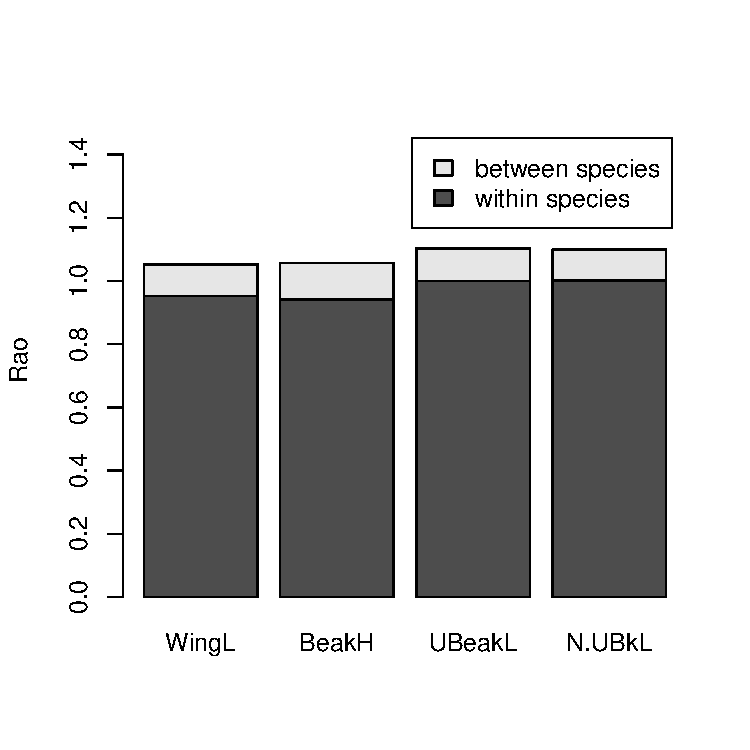
\includegraphics[width=\maxwidth]{figure/unnamed-chunk-21-1} 

}



\end{knitrout}


\subsection{Decomposition of community trait response to environment into intraspecific trait variability, variability due to species turnover and their covariation.}

\textbf{Reference}: Leps, J., de Bello, F., Smilauer, P. and Dolezal, J. (2011) Community trait response to environment: disentangling species turnover vs intraspecific trait variability effects. Ecography, 34, 856-863.

\begin{knitrout}
\definecolor{shadecolor}{rgb}{0.969, 0.969, 0.969}\color{fgcolor}\begin{kframe}
\begin{alltt}
\hlstd{proc.time_decompCTRE} \hlkwb{<-} \hlkwd{proc.time}\hlstd{()} \hlopt{-} \hlstd{ptm}
\hlkwd{barplot}\hlstd{(res.decomp)}
\end{alltt}
\end{kframe}

{\centering 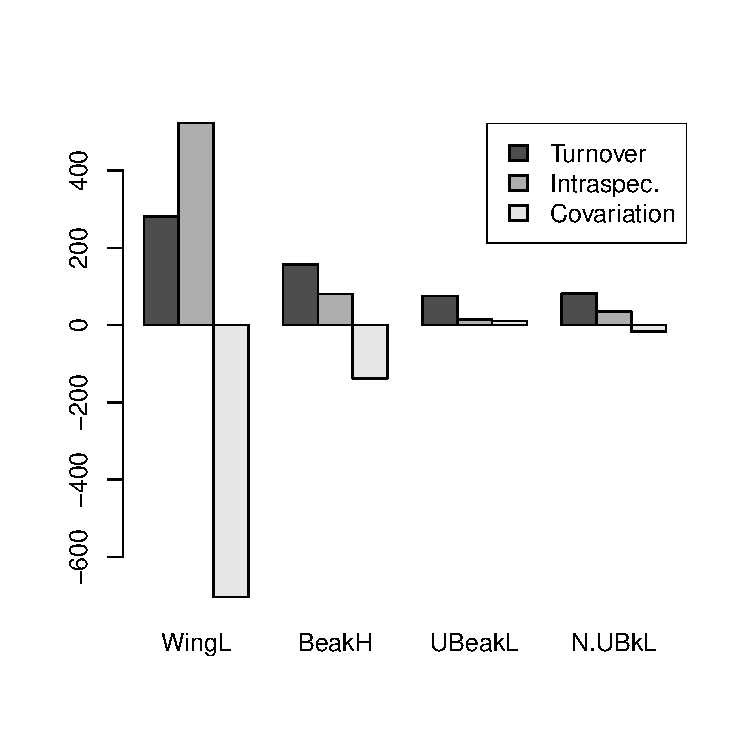
\includegraphics[width=\maxwidth]{figure/unnamed-chunk-22-1} 

}



\end{knitrout}

\begin{knitrout}
\definecolor{shadecolor}{rgb}{0.969, 0.969, 0.969}\color{fgcolor}\begin{kframe}
\begin{alltt}
\hlkwd{par}\hlstd{(}\hlkwc{mfrow} \hlstd{=} \hlkwd{c}\hlstd{(}\hlnum{2}\hlstd{,}\hlnum{2}\hlstd{))}
\hlkwd{barplot}\hlstd{(res.decomp,} \hlkwc{resume} \hlstd{= F)}
\end{alltt}
\end{kframe}

{\centering 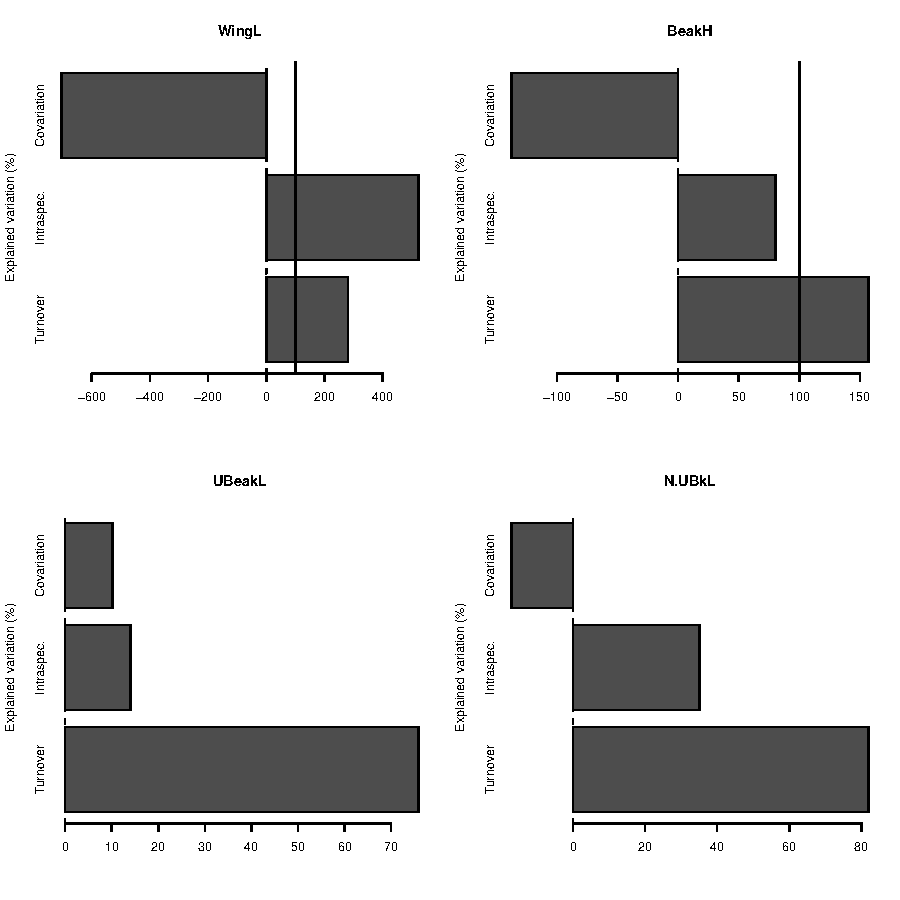
\includegraphics[width=\maxwidth]{figure/unnamed-chunk-23-1} 

}


\begin{kframe}\begin{alltt}
\hlkwd{par}\hlstd{(}\hlkwc{mfrow} \hlstd{=} \hlkwd{c}\hlstd{(}\hlnum{1}\hlstd{,}\hlnum{1}\hlstd{))}
\end{alltt}
\end{kframe}
\end{knitrout}

\newpage

\subsection{Decomposition of traits variances using nested factors}

Variance partitioning across nested scales using the decomposition of variance on restricted maximum likelihood (REML) method (lme function).
~\\

\textbf{Reference}: Messier, J., McGill, B. and Lechowicz, M. (2010) How do traits vary across ecological scales? A case for trait-based ecology. Ecology Letters, 13, 838-848.

\begin{knitrout}
\definecolor{shadecolor}{rgb}{0.969, 0.969, 0.969}\color{fgcolor}\begin{kframe}
\begin{alltt}
\hlstd{vec}\hlkwb{<-} \hlkwd{seq}\hlstd{(}\hlnum{1}\hlstd{,}\hlkwd{length}\hlstd{(sp.finch)}\hlopt{*}\hlnum{2}\hlstd{,} \hlkwc{by} \hlstd{=} \hlnum{2}\hlstd{)}
\hlstd{genus}\hlkwb{<-}\hlkwd{as.vector}\hlstd{(}\hlkwd{unlist}\hlstd{(}\hlkwd{strsplit}\hlstd{(}\hlkwd{as.vector}\hlstd{(sp.finch),}\hlstr{"_"}\hlstd{))[vec])}
\hlstd{fact}\hlkwb{<-}\hlkwd{cbind}\hlstd{(}\hlkwc{genus} \hlstd{=} \hlkwd{as.factor}\hlstd{(genus),}
      \hlkwc{species} \hlstd{=} \hlkwd{as.factor}\hlstd{(}\hlkwd{as.vector}\hlstd{(sp.finch)),}
      \hlkwc{sites} \hlstd{=} \hlkwd{as.factor}\hlstd{(}\hlkwd{as.vector}\hlstd{(ind.plot.finch)))}

\hlstd{ptm} \hlkwb{<-} \hlkwd{proc.time}\hlstd{()}
\hlstd{res.partvar.finch}\hlkwb{<-}\hlkwd{partvar}\hlstd{(}\hlkwc{traits} \hlstd{= traits.finch,} \hlkwc{factors} \hlstd{= fact)}
\hlstd{proc.time_partvar} \hlkwb{<-} \hlkwd{proc.time}\hlstd{()} \hlopt{-} \hlstd{ptm}

\hlstd{res.partvar.finch}
\end{alltt}
\end{kframe}
\end{knitrout}


\begin{knitrout}
\definecolor{shadecolor}{rgb}{0.969, 0.969, 0.969}\color{fgcolor}\begin{kframe}
\begin{alltt}
\hlkwd{par}\hlstd{(}\hlkwc{mfrow} \hlstd{=} \hlkwd{c}\hlstd{(}\hlnum{2}\hlstd{,}\hlnum{2}\hlstd{),} \hlkwc{mai} \hlstd{=} \hlkwd{c}\hlstd{(}\hlnum{0.2}\hlstd{,}\hlnum{0.2}\hlstd{,}\hlnum{0.2}\hlstd{,}\hlnum{0.2}\hlstd{))} \hlcom{#save graphical parameters}
\hlstd{colors}\hlkwb{<-}\hlkwd{c}\hlstd{(}\hlkwd{rgb}\hlstd{(}\hlnum{102}\hlstd{,}\hlnum{167}\hlstd{,}\hlnum{0}\hlstd{,} \hlkwc{maxColorValue} \hlstd{=} \hlnum{255}\hlstd{),}
     \hlkwd{rgb}\hlstd{(}\hlnum{185}\hlstd{,}\hlnum{210}\hlstd{,}\hlnum{0}\hlstd{,} \hlkwc{maxColorValue} \hlstd{=} \hlnum{255}\hlstd{),}
     \hlkwd{rgb}\hlstd{(}\hlnum{98}\hlstd{,}\hlnum{174}\hlstd{,}\hlnum{255}\hlstd{,} \hlkwc{maxColorValue} \hlstd{=} \hlnum{255}\hlstd{),}
     \hlkwd{rgb}\hlstd{(}\hlnum{158}\hlstd{,}\hlnum{30}\hlstd{,}\hlnum{240}\hlstd{,} \hlkwc{maxColorValue} \hlstd{=} \hlnum{255}\hlstd{))}

\hlkwd{piePartvar}\hlstd{(res.partvar.finch,} \hlkwc{col} \hlstd{= colors)}
\end{alltt}
\end{kframe}

{\centering 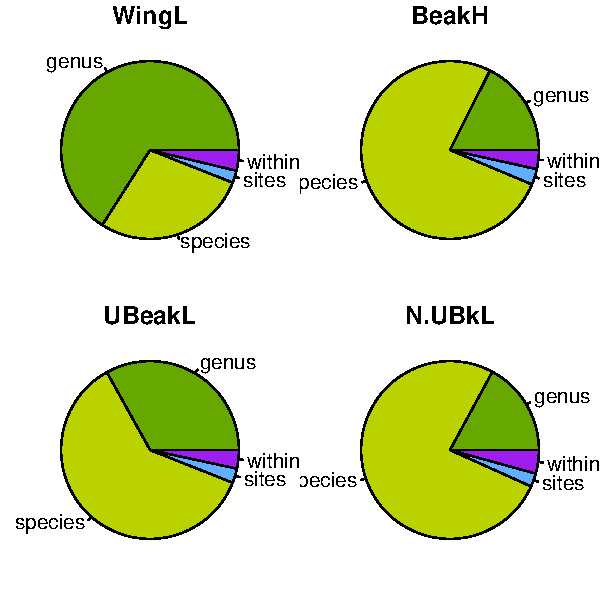
\includegraphics[width=\maxwidth]{figure/unnamed-chunk-25-1} 

}


\begin{kframe}\begin{alltt}
\hlkwd{par}\hlstd{(old.par)} \hlcom{#reset old graphical parameters}
\end{alltt}
\end{kframe}
\end{knitrout}

\begin{knitrout}
\definecolor{shadecolor}{rgb}{0.969, 0.969, 0.969}\color{fgcolor}\begin{kframe}
\begin{alltt}
\hlkwd{barPartvar}\hlstd{(res.partvar.finch,} \hlkwc{col} \hlstd{= colors,} \hlkwc{leg} \hlstd{=} \hlnum{TRUE}\hlstd{)}
\end{alltt}
\end{kframe}

{\centering 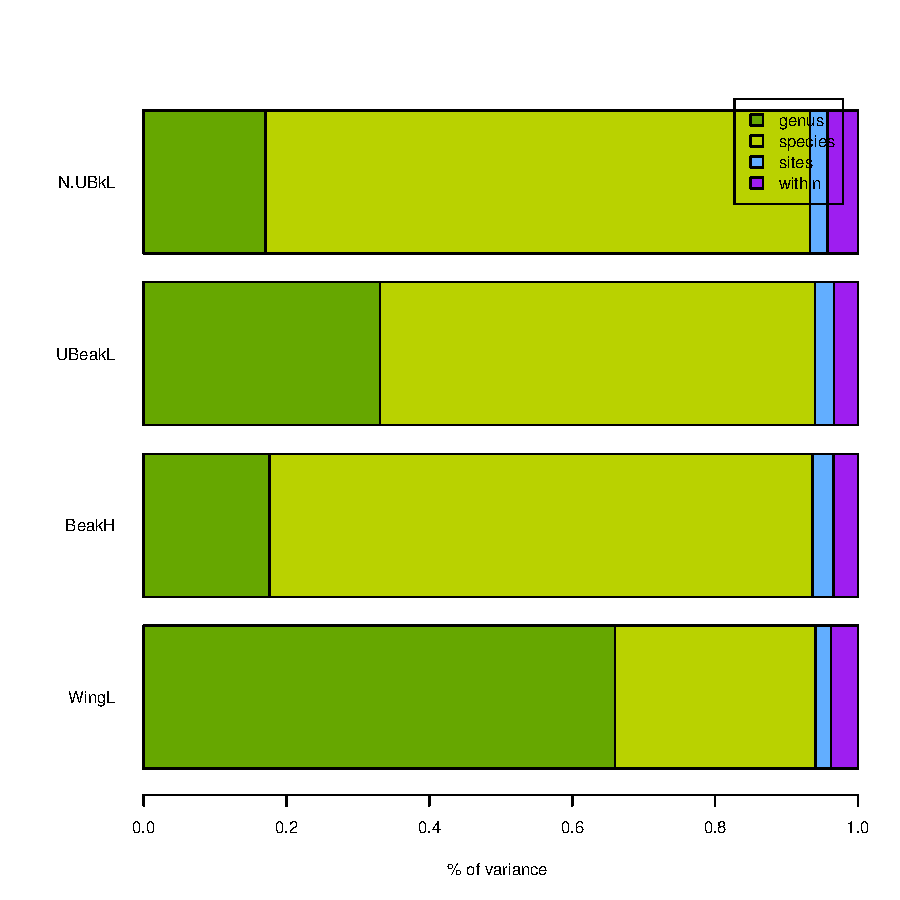
\includegraphics[width=\maxwidth]{figure/unnamed-chunk-26-1} 

}



\end{knitrout}


\newpage

\subsection{Plot the relation between populational trait means and sites traits means.}

For an example of utilisation see: Cornwell, W.K. and Ackerly, D.D., 2009. Community assembly and shifts in plant trait distributions across an environmental gradient in coastal California. Ecological Monographs, 79, 109-126.

\begin{knitrout}
\definecolor{shadecolor}{rgb}{0.969, 0.969, 0.969}\color{fgcolor}\begin{kframe}
\begin{alltt}
\hlkwd{plotSpPop}\hlstd{(traits.finch, ind.plot.finch, sp.finch,} \hlkwc{silent} \hlstd{=} \hlnum{TRUE}\hlstd{)}
\end{alltt}
\end{kframe}
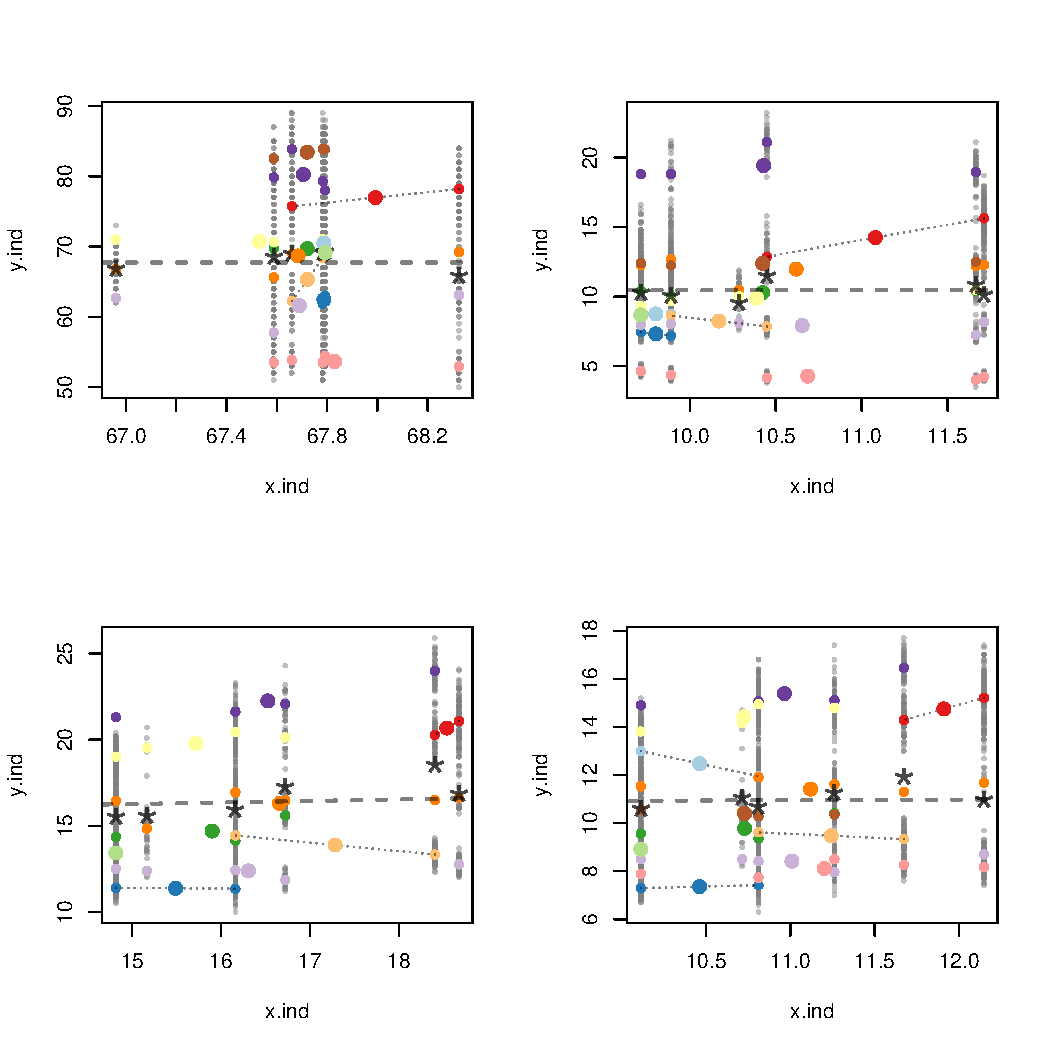
\includegraphics[width=\maxwidth]{figure/unnamed-chunk-27-1} 

\end{knitrout}

If we change the value of two arguments we can see some significant relationships. Here let's try a more permissive threshold: alpha = 10\% instead of 5\% (\texttt{p.val}) and define a lower minimum of values to represent significance  fixed to 3 instead of 10 by default (\texttt{min.ind.signif}). 

\newpage

\begin{knitrout}
\definecolor{shadecolor}{rgb}{0.969, 0.969, 0.969}\color{fgcolor}\begin{kframe}
\begin{alltt}
\hlkwd{plotSpPop}\hlstd{(traits.finch, ind.plot.finch, sp.finch,}
      \hlkwc{p.val} \hlstd{=} \hlnum{0.1}\hlstd{,} \hlkwc{min.ind.signif} \hlstd{=} \hlnum{3}\hlstd{,} \hlkwc{silent} \hlstd{=} \hlnum{TRUE}\hlstd{)}
\end{alltt}
\end{kframe}
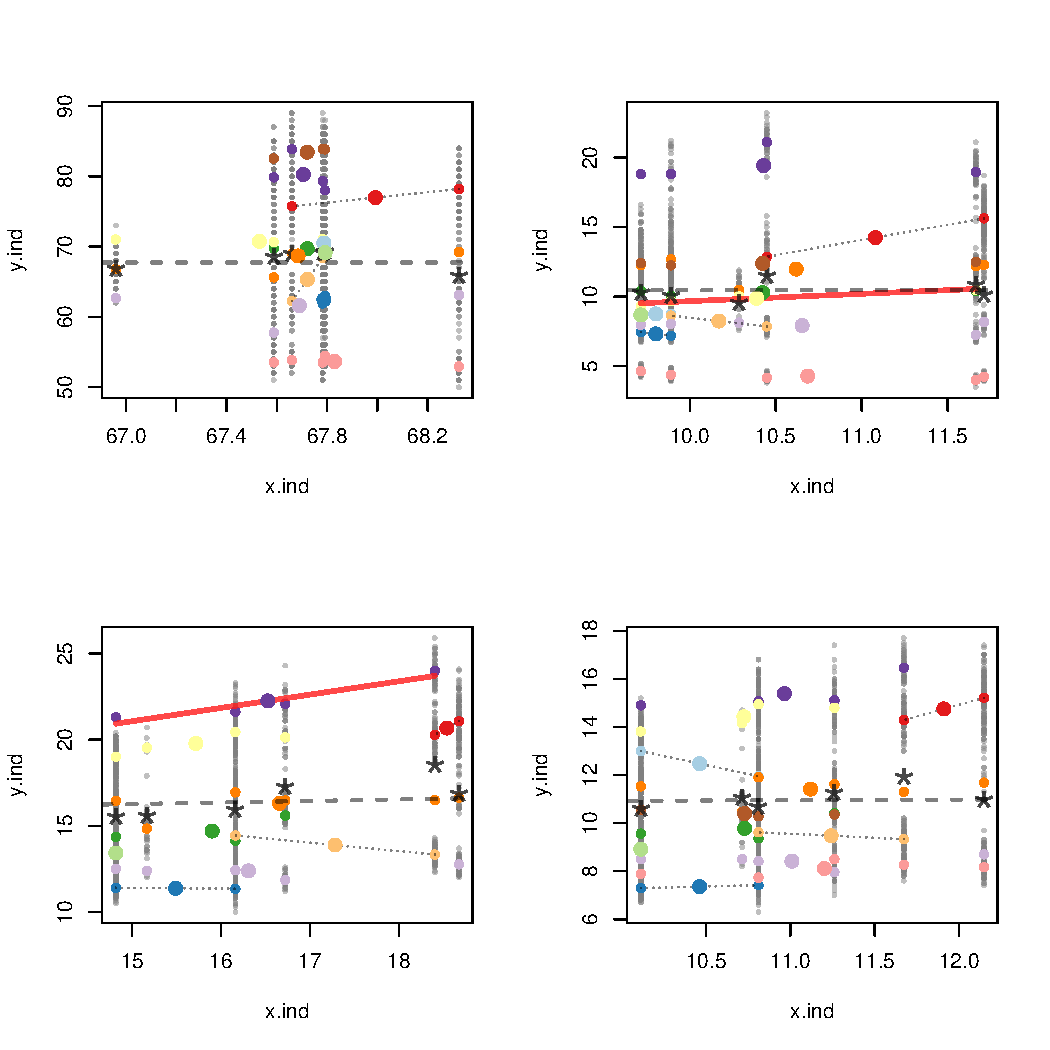
\includegraphics[width=\maxwidth]{figure/unnamed-chunk-28-1} 

\end{knitrout}

\newpage

For a more simple figure, add the option resume = TRUE. 
\begin{knitrout}
\definecolor{shadecolor}{rgb}{0.969, 0.969, 0.969}\color{fgcolor}\begin{kframe}
\begin{alltt}
\hlkwd{plotSpPop}\hlstd{(traits.finch, ind.plot.finch, sp.finch,}
      \hlkwc{silent} \hlstd{=} \hlnum{TRUE}\hlstd{,} \hlkwc{resume} \hlstd{=} \hlnum{TRUE}\hlstd{,} \hlkwc{col.pop} \hlstd{=} \hlstr{"grey"}\hlstd{)}
\end{alltt}
\end{kframe}
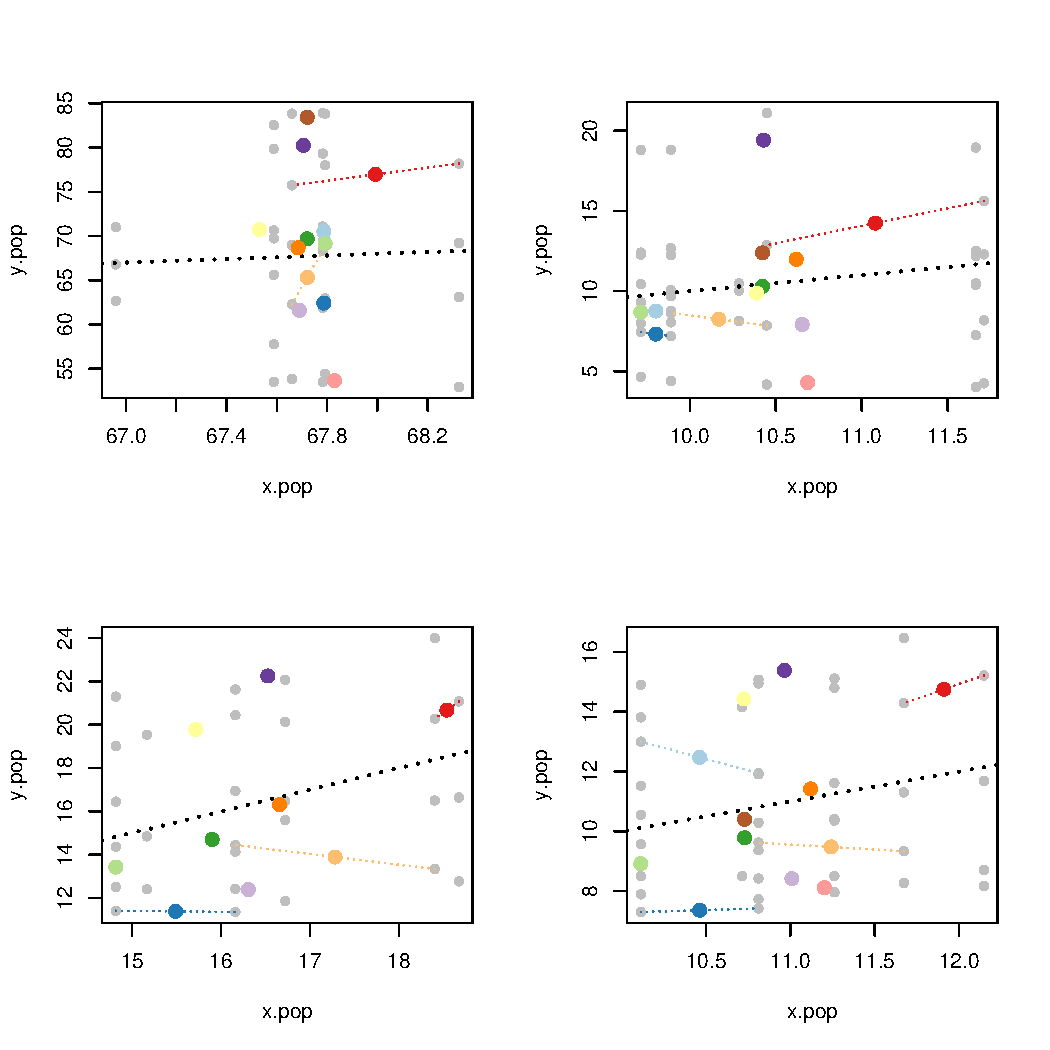
\includegraphics[width=\maxwidth]{figure/unnamed-chunk-29-1} 

\end{knitrout}

If you are fed up with colors, try this:
\begin{knitrout}
\definecolor{shadecolor}{rgb}{0.969, 0.969, 0.969}\color{fgcolor}\begin{kframe}
\begin{alltt}
\hlkwd{plotSpPop}\hlstd{(traits.finch, ind.plot.finch, sp.finch,}
      \hlkwc{silent} \hlstd{=} \hlnum{TRUE}\hlstd{,} \hlkwc{resume} \hlstd{=} \hlnum{TRUE}\hlstd{,} \hlkwc{col.pop} \hlstd{=} \hlstr{"grey"}\hlstd{,} \hlkwc{col.sp} \hlstd{=} \hlstr{"black"}\hlstd{)}
\end{alltt}
\end{kframe}

{\centering 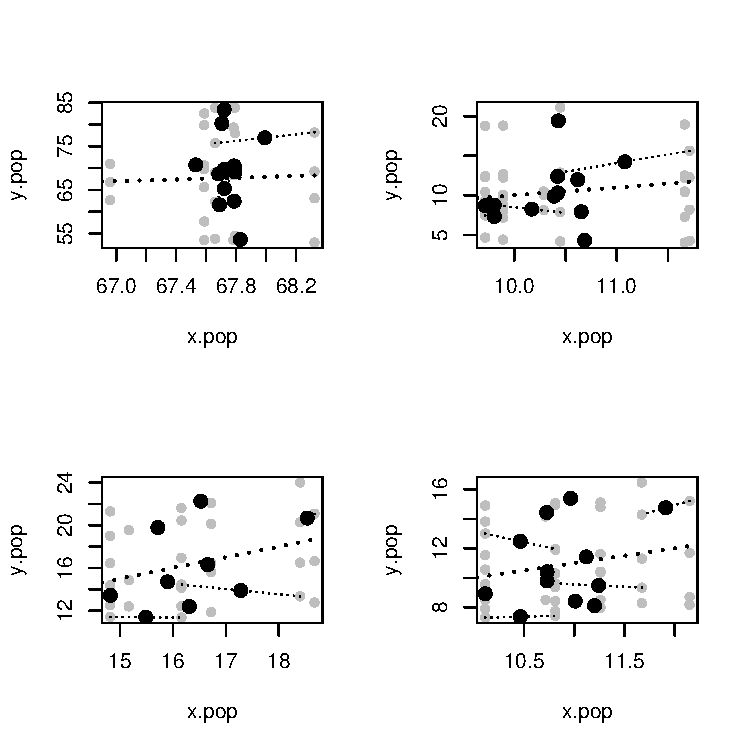
\includegraphics[width=\maxwidth]{figure/unnamed-chunk-30-1} 

}



\end{knitrout}

Again if we change the value of the threshold (\texttt{p.val} = 0.1 and \texttt{min.ind.signif} = 3) we can see some significant relationships.

\begin{knitrout}
\definecolor{shadecolor}{rgb}{0.969, 0.969, 0.969}\color{fgcolor}\begin{kframe}
\begin{alltt}
\hlkwd{plotSpPop}\hlstd{(traits.finch, ind.plot.finch, sp.finch,}
      \hlkwc{silent} \hlstd{=} \hlnum{TRUE}\hlstd{,} \hlkwc{resume} \hlstd{=} \hlnum{TRUE}\hlstd{,} \hlkwc{col.pop} \hlstd{=} \hlstr{"grey"}\hlstd{,} \hlkwc{col.sp} \hlstd{=} \hlstr{"black"}\hlstd{,}
      \hlkwc{p.val} \hlstd{=} \hlnum{0.1}\hlstd{,} \hlkwc{min.ind.signif} \hlstd{=} \hlnum{3}\hlstd{)}
\end{alltt}
\end{kframe}

{\centering 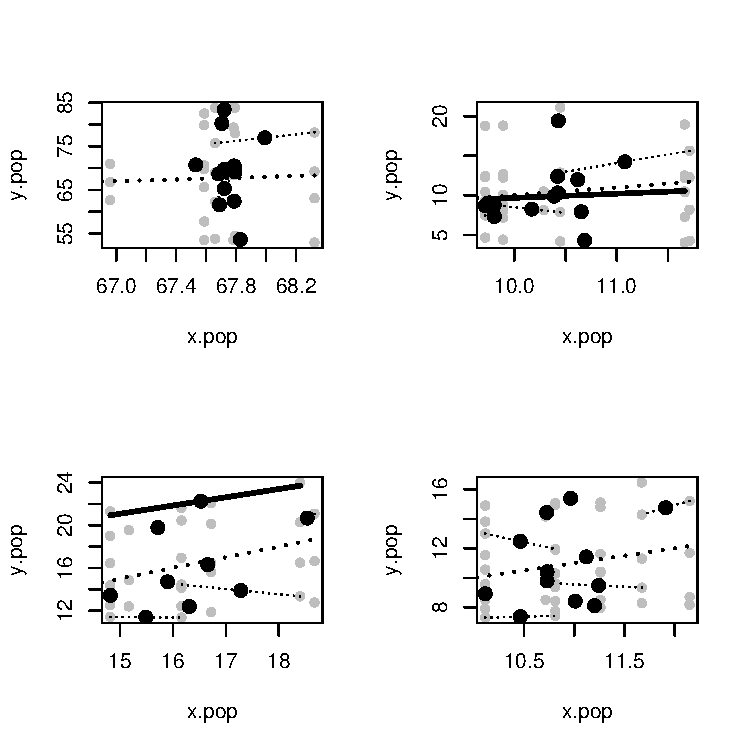
\includegraphics[width=\maxwidth]{figure/unnamed-chunk-31-1} 

}



\end{knitrout}


\newpage

%%%%%%%%%%%%%%%%
\section{Test of community assembly}
%%%%%%%%%%%%%%%%

\subsection{Ratio of variances: T-statistics}

The function \texttt{Tstat} computes observed T-statistics (T for Traits; Violle et al (2012)) as three ratios of variance, namely $T_{IP/IC}$, $T_{IC/IR}$ and $T_{PC/PR}$. This function can also return the distribution of these three statistics under the three associated null models (respectively \textbf{local}, \textbf{regional.ind} and \textbf{regional.pop}).
~\\

\textbf{Reference}: Violle, C., Enquist, B.J., McGill, B.J., Jiang, L., Albert, C., Hulshof, C., Jung, V. and Messier, J. (2012) The return of the variance: intraspecific variability in community ecology. Trends in Ecology and Evolution, 27, 244-252.

\begin{knitrout}
\definecolor{shadecolor}{rgb}{0.969, 0.969, 0.969}\color{fgcolor}\begin{kframe}
\begin{alltt}
\hlstd{res.finch}\hlkwb{<-}\hlkwd{Tstats}\hlstd{(traits.finch,} \hlkwc{ind.plot} \hlstd{= ind.plot.finch,} \hlkwc{sp} \hlstd{= sp.finch,}
         \hlkwc{nperm} \hlstd{=} \hlnum{99}\hlstd{,} \hlkwc{print} \hlstd{=} \hlnum{FALSE}\hlstd{)}
\hlstd{res.finch}
\end{alltt}
\begin{verbatim}
## 	##################
## 	# T-statistiques #
## 	##################
## class: Tstats
## $call: Tstats(traits = traits.finch, ind.plot = ind.plot.finch, sp = sp.finch, 
##     nperm = 99, printprogress = FALSE)
## 
## ###############
## $Tstats: list of observed and null T-statistics
## 
## Observed values
## 	$T_IP.IC: ratio of within-population variance to total within-community variance
## 	$T_IC.IR: community-wide variance relative to the total variance in the regional pool
## 	$T_PC.PR: inter-community variance relative to the total variance in the regional pool
## 
## Null values, number of permutation: 99
## 	$T_IP.IC_nm: distribution of T_IP.IC value under the null model local
## 	$T_IC.IR_nm: distribution of T_IC.IR value under the null model regional.ind 
## 	$T_PC.PR_nm: distribution of T_PC.PR value under the null model regional.pop
## 
## ###############
## $variances: list of observed and null variances
## 
## ###############
## data used
##   data      class      dim   
## 1 $traits   data.frame 2513,4
## 2 $ind.plot factor     2513  
## 3 $sp       factor     2513  
##   content                                             
## 1 traits data                                         
## 2 name of the plot in which the individual is         
## 3 groups (e.g. species) which the individual belong to
## 
## ###############
## others
## 	$namestraits: 4 traits
## [1] "WingL"  "BeakH"  "UBeakL" "N.UBkL"
## 
## 	$sites_richness:
## 	ind.plot
##     DMaj    EspHd FlorChrl  GnovTwr MrchBndl SCruInde 
##       50      267      981      258      270      687
\end{verbatim}
\end{kframe}
\end{knitrout}



\subsubsection{S3 methods for class Tstats}
Tstats class is associated to S3 methods plot, barplot, print and summary. We have already used the print function in the above script line. Now, how to plot the result of the function \texttt{Tstats}?

We can represent observed values thanks to the \texttt{barplot} function.
\begin{knitrout}
\definecolor{shadecolor}{rgb}{0.969, 0.969, 0.969}\color{fgcolor}\begin{kframe}
\begin{alltt}
\hlkwd{barplot}\hlstd{(res.finch,} \hlkwc{ylim} \hlstd{=} \hlkwd{c}\hlstd{(}\hlnum{0}\hlstd{,}\hlnum{3.5}\hlstd{))}
\end{alltt}
\end{kframe}

{\centering 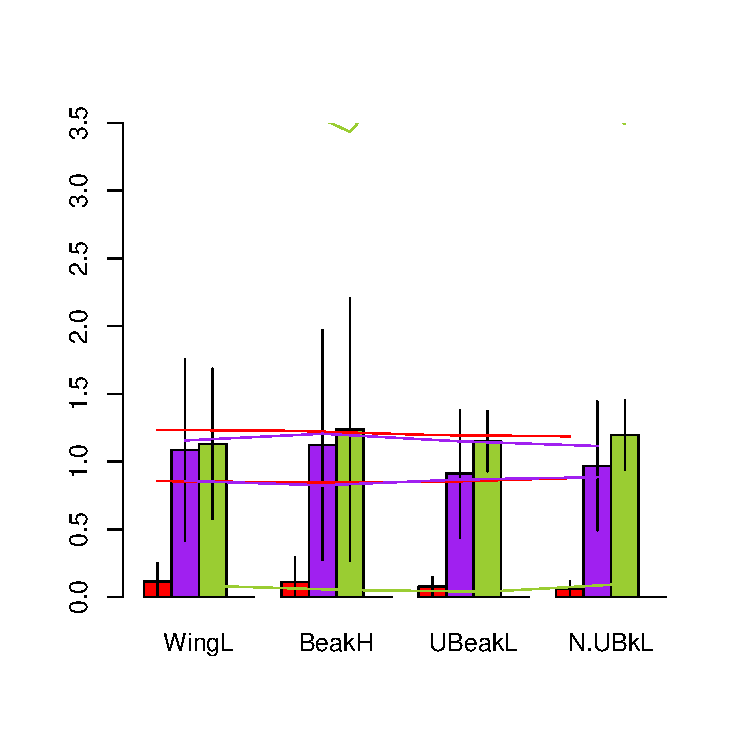
\includegraphics[width=\maxwidth]{figure/unnamed-chunk-33-1} 

}



\end{knitrout}

One can be more interested in the significance  and the effect size available thanks to null model. In that case, the standardized effect size can be easily plot. Note that the function \texttt{ses} can be use directly to calculate standardized effect size without plotting. The Standardized Effect Size (ses) is define as : 

\begin{center}
$$ SES = (I_{obs} – I{_sim}) / \delta_{sim} $$
\end{center}

where $I_{obs}$ is the observed value, $I_{sim}$ the mean of values calculated from the null model and $\delta_{sim}$ the standard deviation of these simulated values.


\begin{knitrout}
\definecolor{shadecolor}{rgb}{0.969, 0.969, 0.969}\color{fgcolor}\begin{kframe}
\begin{alltt}
\hlkwd{plot}\hlstd{(res.finch)}
\end{alltt}
\end{kframe}

{\centering 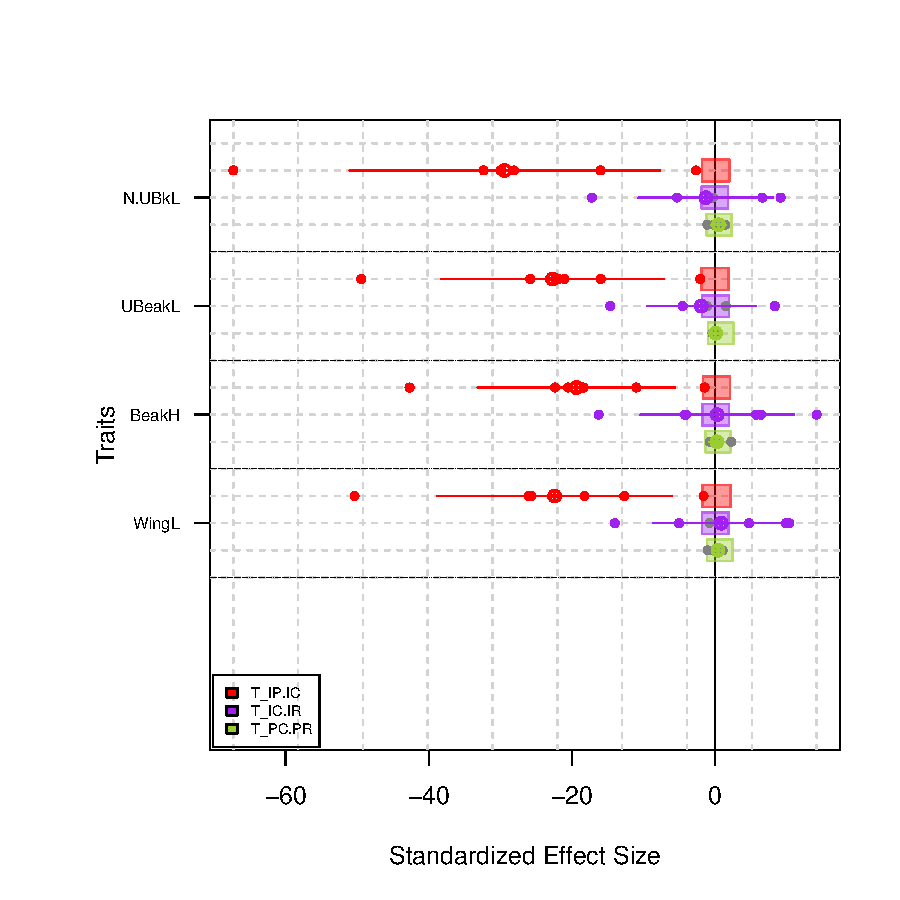
\includegraphics[width=\maxwidth]{figure/unnamed-chunk-34-1} 

}



\end{knitrout}

There is multiple kind of representation avaible.
\begin{knitrout}
\definecolor{shadecolor}{rgb}{0.969, 0.969, 0.969}\color{fgcolor}\begin{kframe}
\begin{alltt}
\hlkwd{plot}\hlstd{(res.finch,} \hlkwc{type} \hlstd{=} \hlstr{"simple"}\hlstd{)}
\end{alltt}
\end{kframe}

{\centering 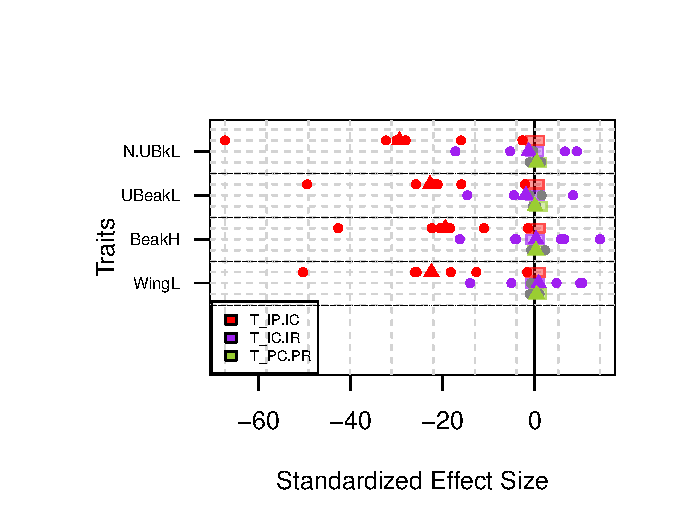
\includegraphics[width=\maxwidth]{figure/unnamed-chunk-35-1} 

}


\begin{kframe}\begin{alltt}
\hlkwd{plot}\hlstd{(res.finch,} \hlkwc{type} \hlstd{=} \hlstr{"simple_range"}\hlstd{)}
\end{alltt}
\end{kframe}

{\centering 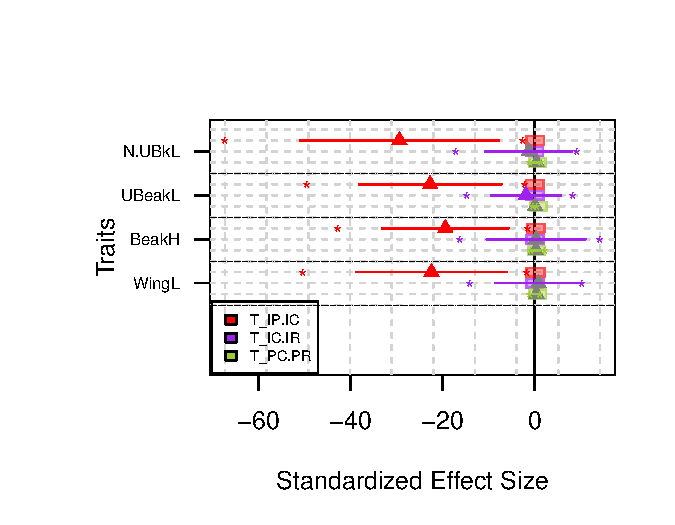
\includegraphics[width=\maxwidth]{figure/unnamed-chunk-35-2} 

}


\begin{kframe}\begin{alltt}
\hlkwd{plot}\hlstd{(res.finch,} \hlkwc{type} \hlstd{=} \hlstr{"barplot"}\hlstd{)}
\end{alltt}
\end{kframe}

{\centering 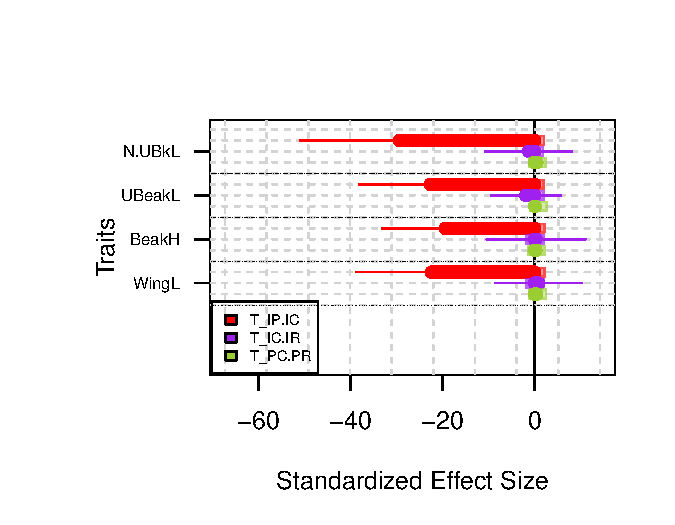
\includegraphics[width=\maxwidth]{figure/unnamed-chunk-35-3} 

}



\end{knitrout}

If you want to specifically look at traits or sites statistics, use the argument \texttt{type = "bytraits"} or \texttt{"bysites"}.
\begin{knitrout}
\definecolor{shadecolor}{rgb}{0.969, 0.969, 0.969}\color{fgcolor}\begin{kframe}
\begin{alltt}
\hlkwd{par}\hlstd{(}\hlkwc{mfrow}\hlstd{=}\hlkwd{c}\hlstd{(}\hlnum{2}\hlstd{,}\hlnum{2}\hlstd{))}

\hlkwd{plot}\hlstd{(res.finch,} \hlkwc{type} \hlstd{=} \hlstr{"bytraits"}\hlstd{)}
\end{alltt}
\end{kframe}

{\centering 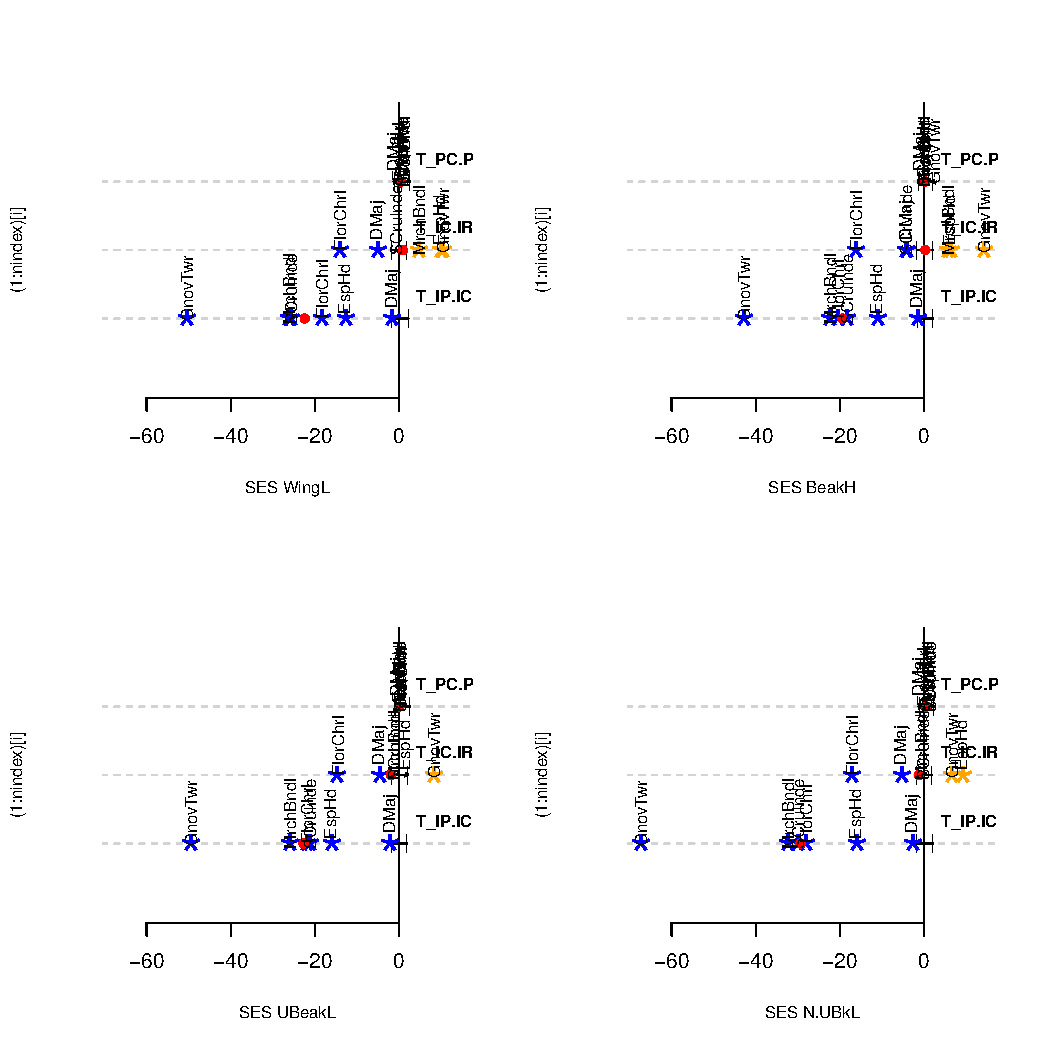
\includegraphics[width=\maxwidth]{figure/unnamed-chunk-36-1} 

}


\begin{kframe}\begin{alltt}
\hlkwd{plot}\hlstd{(res.finch,} \hlkwc{type} \hlstd{=} \hlstr{"bysites"}\hlstd{)}
\end{alltt}
\end{kframe}

{\centering 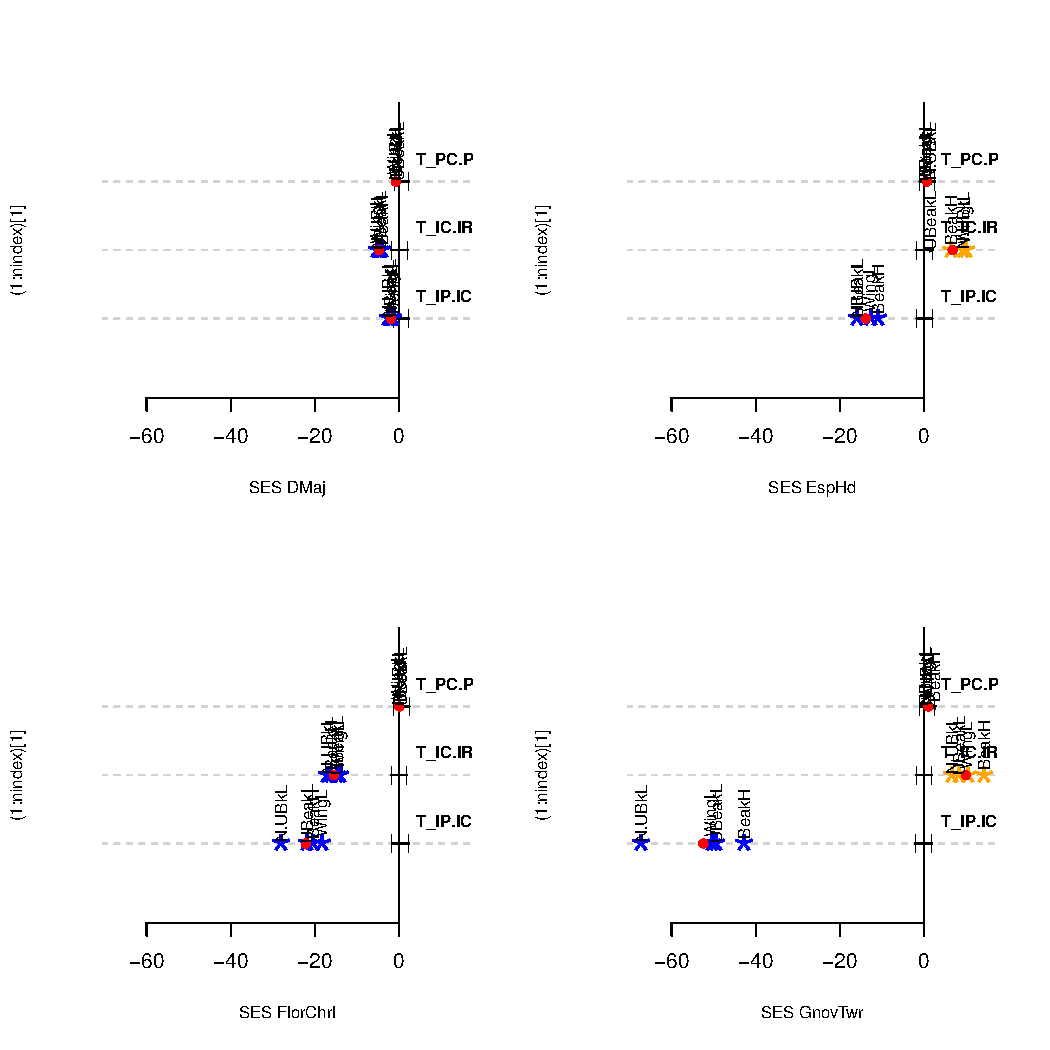
\includegraphics[width=\maxwidth]{figure/unnamed-chunk-36-2} 

}


\begin{kframe}\begin{alltt}
\hlkwd{par}\hlstd{(old.par)} \hlcom{# reset default graphical parameters}
\end{alltt}
\end{kframe}

{\centering 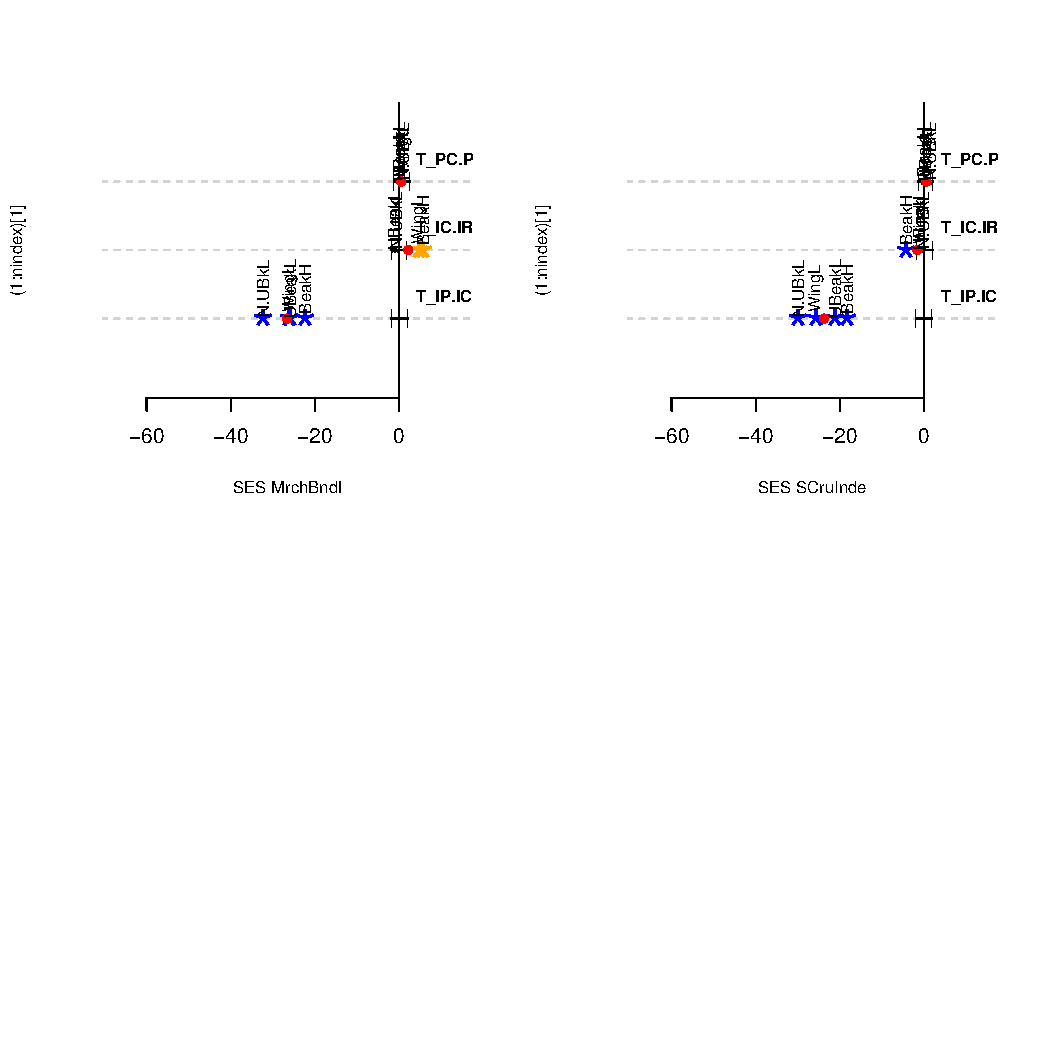
\includegraphics[width=\maxwidth]{figure/unnamed-chunk-36-3} 

}



\end{knitrout}

\newpage

\begin{knitrout}
\definecolor{shadecolor}{rgb}{0.969, 0.969, 0.969}\color{fgcolor}\begin{kframe}
\begin{alltt}
\hlkwd{summary}\hlstd{(res.finch)} \hlcom{#S3 summary method for class Tstats}
\end{alltt}
\begin{verbatim}
## [1] "Observed values"
## $T_IP.IC
##      WingL             BeakH             UBeakL            N.UBkL       
##  Min.   :0.03435   Min.   :0.01528   Min.   :0.02669   Min.   :0.02385  
##  1st Qu.:0.04365   1st Qu.:0.01907   1st Qu.:0.04170   1st Qu.:0.03670  
##  Median :0.06448   Median :0.04003   Median :0.05445   Median :0.04035  
##  Mean   :0.11608   Mean   :0.10944   Mean   :0.07640   Mean   :0.06147  
##  3rd Qu.:0.10115   3rd Qu.:0.05802   3rd Qu.:0.06289   3rd Qu.:0.04939  
##  Max.   :0.38311   Max.   :0.48519   Max.   :0.21962   Max.   :0.17637  
## 
## $T_IC.IR
##      WingL             BeakH             UBeakL           N.UBkL      
##  Min.   :0.09246   Min.   :0.06316   Min.   :0.2461   Min.   :0.2569  
##  1st Qu.:0.67385   1st Qu.:0.49130   1st Qu.:0.6684   1st Qu.:0.7238  
##  Median :1.17073   Median :1.18311   Median :0.9442   Median :0.9800  
##  Mean   :1.08518   Mean   :1.12359   Mean   :0.9109   Mean   :0.9677  
##  3rd Qu.:1.62569   3rd Qu.:1.62423   3rd Qu.:1.0803   3rd Qu.:1.3144  
##  Max.   :1.79158   Max.   :2.28021   Max.   :1.6287   Max.   :1.5250  
## 
## $T_PC.PR
##      WingL            BeakH             UBeakL           N.UBkL      
##  Min.   :0.2261   Min.   :0.08685   Min.   :0.9328   Min.   :0.9356  
##  1st Qu.:0.8981   1st Qu.:0.86252   1st Qu.:0.9828   1st Qu.:1.0388  
##  Median :1.2233   Median :1.05894   Median :1.1249   Median :1.0992  
##  Mean   :1.1303   Mean   :1.23699   Mean   :1.1488   Mean   :1.1955  
##  3rd Qu.:1.4737   3rd Qu.:1.32864   3rd Qu.:1.2148   3rd Qu.:1.3513  
##  Max.   :1.7622   Max.   :3.00163   Max.   :1.5301   Max.   :1.5852  
## 
## [1] "null values"
## $T_IP.IC_nm
##    Min. 1st Qu.  Median    Mean 3rd Qu.    Max. 
##  0.3859  0.9662  0.9987  0.9997  1.0270  2.6290 
## 
## $T_IC.IR_nm
##    Min. 1st Qu.  Median    Mean 3rd Qu.    Max. 
##  0.4624  0.9596  0.9992  1.0020  1.0420  1.5160 
## 
## $T_PC.PR_nm
##    Min. 1st Qu.  Median    Mean 3rd Qu.    Max.    NA's 
##  0.0000  0.3473  0.7480  1.1690  1.4250 11.6300     189
\end{verbatim}
\end{kframe}
\end{knitrout}


\begin{knitrout}
\definecolor{shadecolor}{rgb}{0.969, 0.969, 0.969}\color{fgcolor}\begin{kframe}
\begin{alltt}
\hlkwd{attributes}\hlstd{(}\hlkwd{sum_Tstats}\hlstd{(res.finch))} \hlcom{#Another mean to summarize Tstatistics}
\end{alltt}
\begin{verbatim}
## $names
## [1] "p.value" "percent" "sites"   "binary"
\end{verbatim}
\begin{alltt}
\hlkwd{head}\hlstd{(}\hlkwd{sum_Tstats}\hlstd{(res.finch)}\hlopt{$}\hlstd{p.value,} \hlnum{10}\hlstd{)}
\end{alltt}
\begin{verbatim}
##             WingL BeakH UBeakL N.UBkL
## T_IP.IC.inf  0.01  0.03   0.01   0.01
## T_IP.IC.inf  0.01  0.01   0.01   0.01
## T_IP.IC.inf  0.01  0.01   0.01   0.01
## T_IP.IC.inf  0.01  0.01   0.01   0.01
## T_IP.IC.inf  0.01  0.01   0.01   0.01
## T_IP.IC.inf  0.01  0.01   0.01   0.01
## T_IP.IC.sup  1.00  0.98   1.00   1.00
## T_IP.IC.sup  1.00  1.00   1.00   1.00
## T_IP.IC.sup  1.00  1.00   1.00   1.00
## T_IP.IC.sup  1.00  1.00   1.00   1.00
\end{verbatim}
\end{kframe}
\end{knitrout}

\newpage

\subsubsection{Plot T-statistics correlations}

We can also see T-statistics correlations and theirs correlation with others variables (e.g. a gradient variable, or the species richness).

\begin{knitrout}
\definecolor{shadecolor}{rgb}{0.969, 0.969, 0.969}\color{fgcolor}\begin{kframe}
\begin{alltt}
\hlkwd{par}\hlstd{(}\hlkwc{mfrow} \hlstd{=} \hlkwd{c}\hlstd{(}\hlnum{2}\hlstd{,}\hlnum{3}\hlstd{))}
\hlkwd{plotCorTstats}\hlstd{(res.finch,} \hlkwc{plot.ask} \hlstd{=} \hlnum{FALSE}\hlstd{,} \hlkwc{multipanel} \hlstd{= F)}
\end{alltt}
\end{kframe}
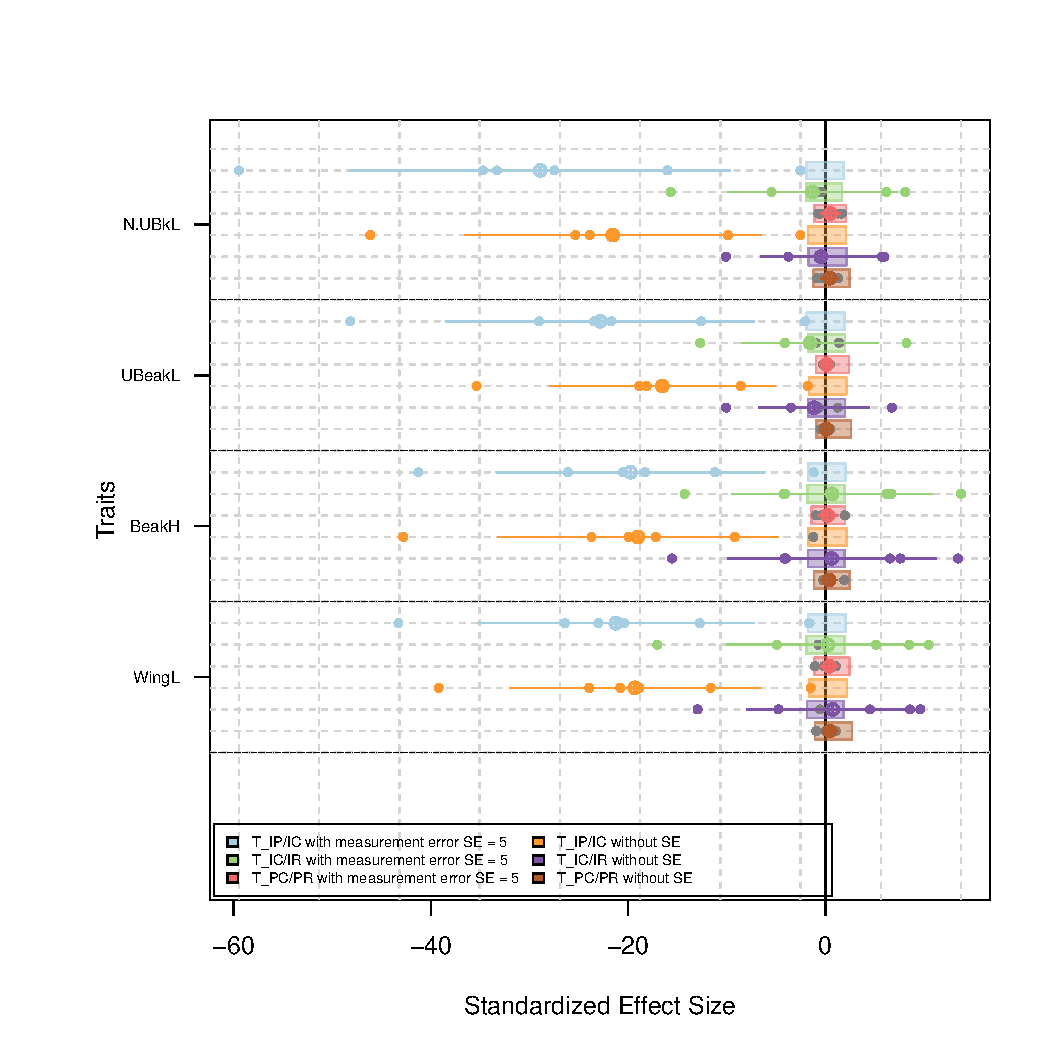
\includegraphics[width=\maxwidth]{figure/unnamed-chunk-39-1} 

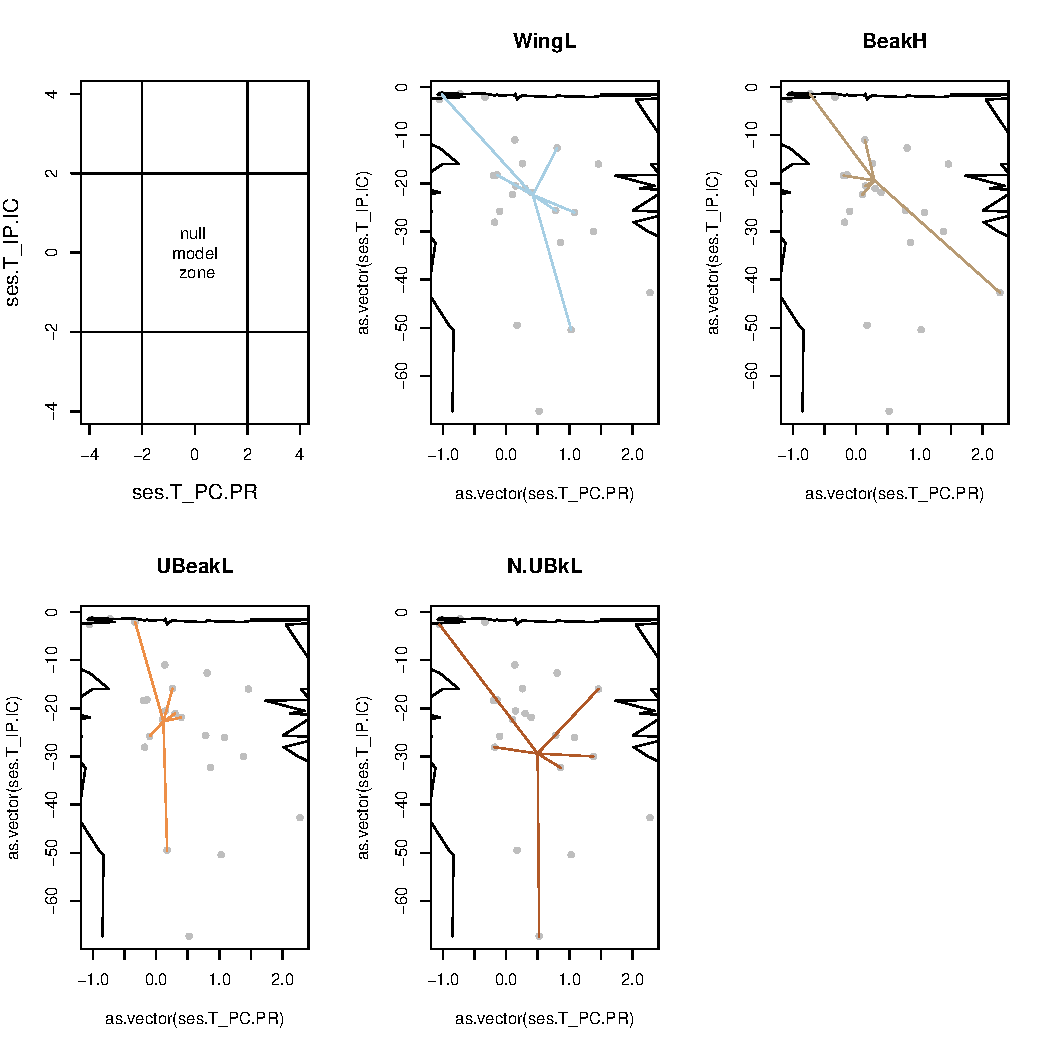
\includegraphics[width=\maxwidth]{figure/unnamed-chunk-39-2} 

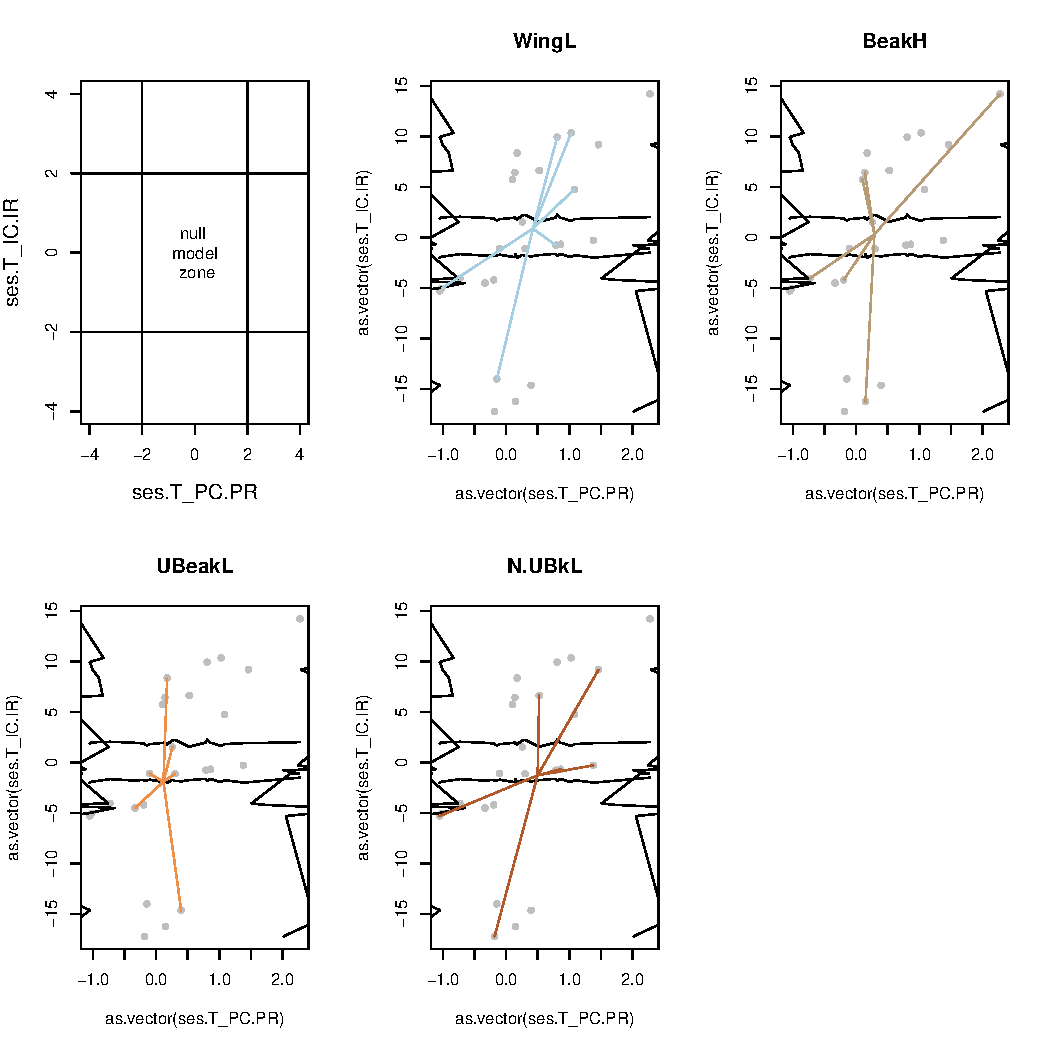
\includegraphics[width=\maxwidth]{figure/unnamed-chunk-39-3} 

\end{knitrout}

Here we plot T-statistics (in the standardized effect size SES form) in function of species richness by sites.

\begin{knitrout}
\definecolor{shadecolor}{rgb}{0.969, 0.969, 0.969}\color{fgcolor}\begin{kframe}
\begin{alltt}
\hlkwd{par}\hlstd{(}\hlkwc{mfrow} \hlstd{=} \hlkwd{c}\hlstd{(}\hlnum{2}\hlstd{,}\hlnum{2}\hlstd{))}
\hlstd{species.richness}\hlkwb{<-}\hlkwd{table}\hlstd{(ind.plot.finch)}
\hlkwd{plotSESvar}\hlstd{(}\hlkwd{as.listofindex}\hlstd{(}\hlkwd{list}\hlstd{(res.finch)), species.richness,}
       \hlkwc{multipanel} \hlstd{= F)}
\end{alltt}
\end{kframe}
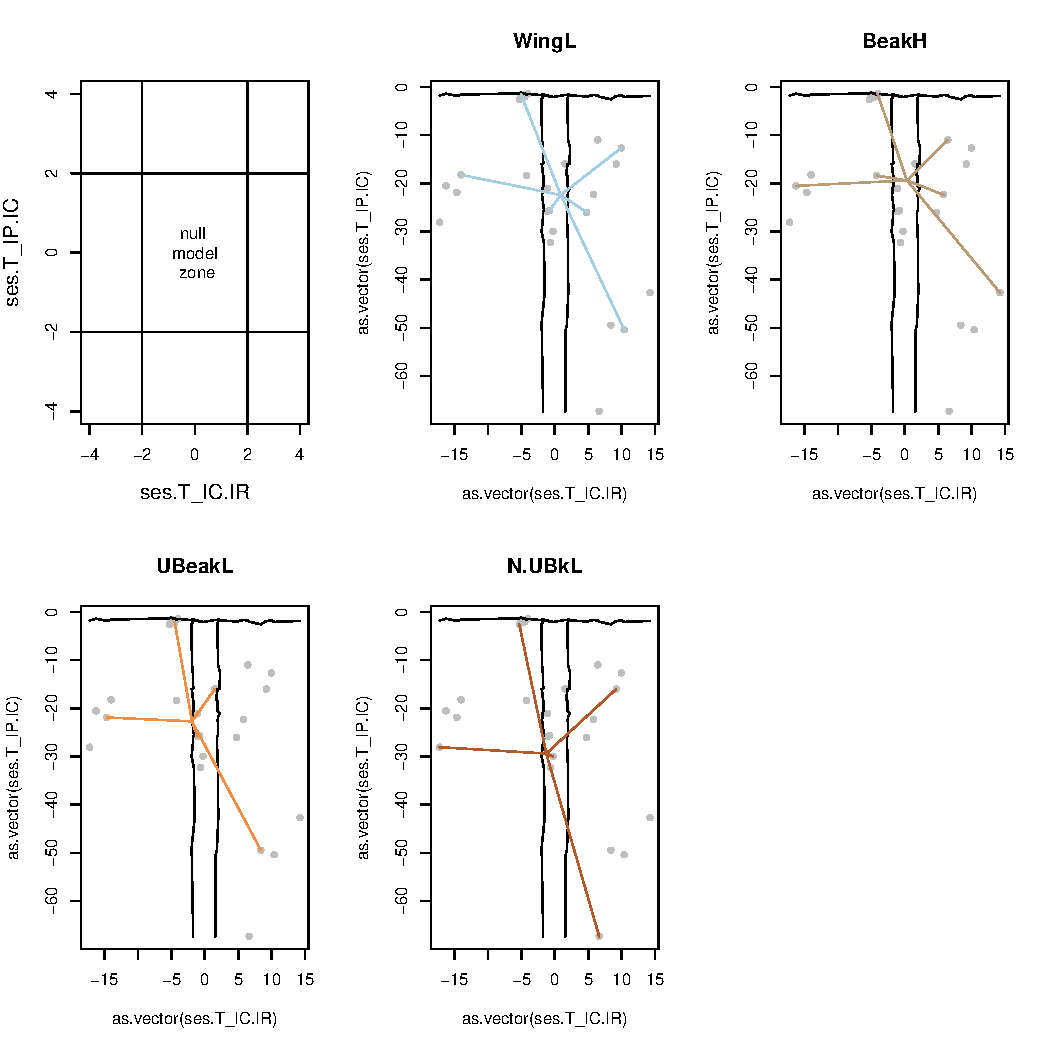
\includegraphics[width=\maxwidth]{figure/unnamed-chunk-40-1} 

\end{knitrout}

Same plot with \texttt{resume = TRUE}.

\begin{knitrout}
\definecolor{shadecolor}{rgb}{0.969, 0.969, 0.969}\color{fgcolor}\begin{kframe}
\begin{alltt}
\hlkwd{par}\hlstd{(}\hlkwc{mfrow} \hlstd{=} \hlkwd{c}\hlstd{(}\hlnum{2}\hlstd{,}\hlnum{2}\hlstd{))}
\hlkwd{plotSESvar}\hlstd{(}\hlkwd{as.listofindex}\hlstd{(}\hlkwd{list}\hlstd{(res.finch)), species.richness,}
       \hlkwc{resume} \hlstd{= T,} \hlkwc{multipanel} \hlstd{= F)}
\end{alltt}
\end{kframe}
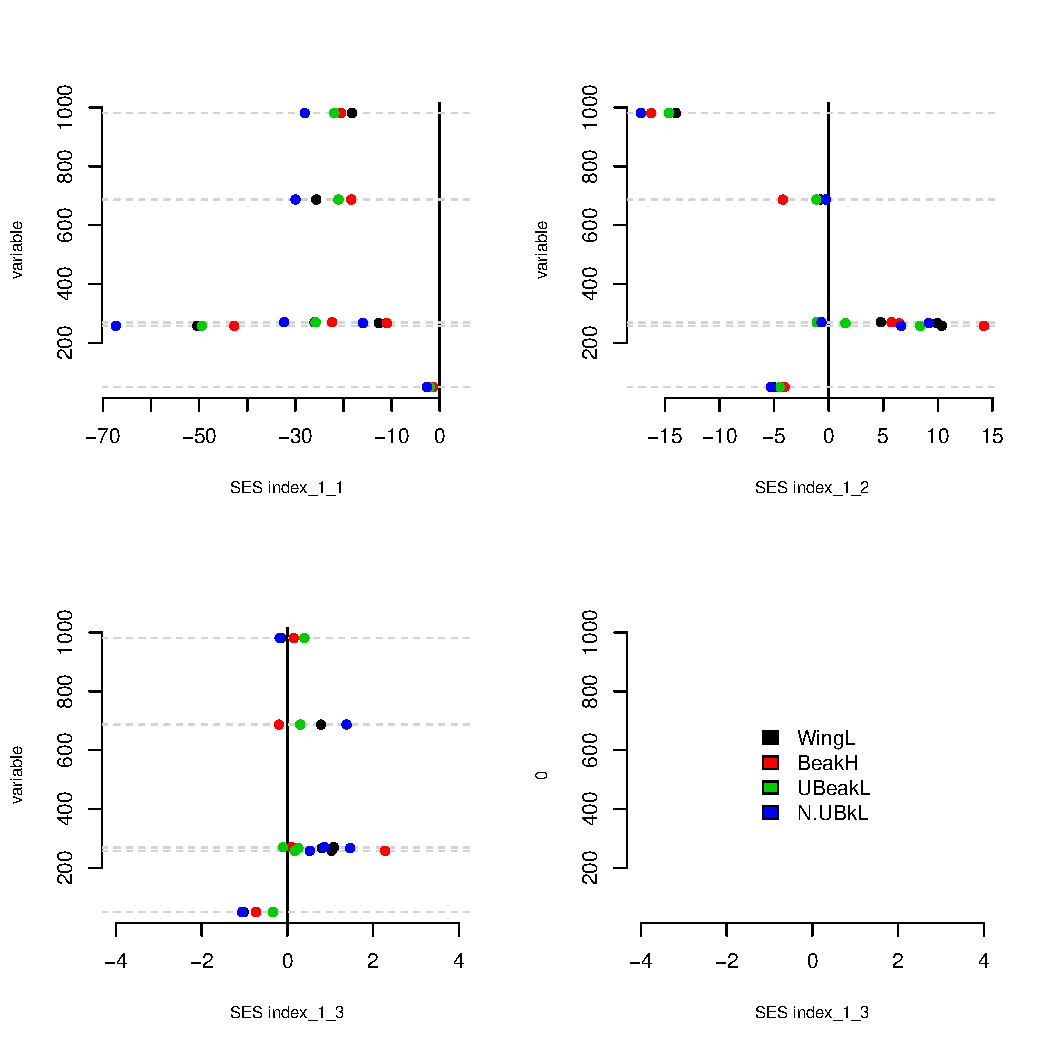
\includegraphics[width=\maxwidth]{figure/unnamed-chunk-41-1} 
\begin{kframe}\begin{alltt}
\hlkwd{par}\hlstd{(}\hlkwc{mfrow} \hlstd{=} \hlkwd{c}\hlstd{(}\hlnum{1}\hlstd{,}\hlnum{1}\hlstd{))}
\end{alltt}
\end{kframe}
\end{knitrout}


\newpage
\subsection{Others univariates or multivariates metrics: function \texttt{ComIndex} and \texttt{ComIndexMulti}}

The function \texttt{ComIndex} allow choosing your own function (like mean, range, variance, ...) to calculate customize metrics. Here \texttt{CVNND} refers to the Coefficient of Variation of the Nearest Neighborhood Distance. \texttt{ComIndexMulti} do the same things for multivariate metrics. 

\begin{knitrout}
\definecolor{shadecolor}{rgb}{0.969, 0.969, 0.969}\color{fgcolor}\begin{kframe}
\begin{alltt}
\hlcom{#Define the functions you want to calculate}
\hlstd{funct}\hlkwb{<-}\hlkwd{c}\hlstd{(}\hlstr{"mean(x, na.rm = T)"}\hlstd{,} \hlstr{"kurtosis(x, na.rm = T)"}\hlstd{,}
     \hlstr{"max(x, na.rm = T) - min(x, na.rm = T)"}\hlstd{,} \hlstr{"CVNND(x)"} \hlstd{)}

\hlcom{#Test against the null model regional.ind}
\hlstd{res.finch.sp_regional.ind}\hlkwb{<-}\hlkwd{ComIndex}\hlstd{(}\hlkwc{traits} \hlstd{= traits.finch,} \hlkwc{index} \hlstd{= funct,} \hlkwc{sp} \hlstd{= sp.finch,}
                           \hlkwc{nullmodels} \hlstd{=} \hlstr{"regional.ind"}\hlstd{,} \hlkwc{ind.plot} \hlstd{= ind.plot.finch,}
                            \hlkwc{nperm} \hlstd{=} \hlnum{99}\hlstd{,} \hlkwc{print} \hlstd{=} \hlnum{FALSE}\hlstd{)}

\hlcom{#Test against the null model regional.pop}
\hlcom{#Individuals values are transformed in populational values}
\hlstd{res.finch.sp_regional.pop}\hlkwb{<-}\hlkwd{ComIndex}\hlstd{(}\hlkwc{traits} \hlstd{= traits.finch,} \hlkwc{index} \hlstd{= funct,} \hlkwc{sp} \hlstd{= sp.finch,}
               \hlkwc{nullmodels} \hlstd{=} \hlstr{"regional.pop"}\hlstd{,} \hlkwc{ind.plot} \hlstd{= ind.plot.finch,}
               \hlkwc{nperm} \hlstd{=} \hlnum{99}\hlstd{,} \hlkwc{print} \hlstd{=} \hlnum{FALSE}\hlstd{)}
\end{alltt}
\end{kframe}
\end{knitrout}

These two functions allows to calculate  index by sites for example using \code{"tapply(x, sites, mean)"}.

\begin{knitrout}
\definecolor{shadecolor}{rgb}{0.969, 0.969, 0.969}\color{fgcolor}\begin{kframe}
\begin{alltt}
\hlstd{funct.1}\hlkwb{<-}\hlkwd{c}\hlstd{(}\hlstr{"tapply(x, ind.plot.finch, function(x) mean(x, na.rm = T))"}\hlstd{,}
     \hlstr{"tapply(x, ind.plot.finch, function(x) kurtosis(x, na.rm = T))"}\hlstd{,}
     \hlstr{"tapply(x, ind.plot.finch, function(x) max(x, na.rm = T)-min(x, na.rm = T))"}\hlstd{,}
     \hlstr{"tapply(x, ind.plot.finch, function(x) CVNND(x))"} \hlstd{)}

\hlkwd{IndexByGroups}\hlstd{(funct,} \hlstr{"ind.plot.finch"}\hlstd{)}
\end{alltt}
\begin{verbatim}
## [1] "tapply(x, ind.plot.finch, function(x) mean(x, na.rm = T))"                   
## [2] "tapply(x, ind.plot.finch, function(x) kurtosis(x, na.rm = T))"               
## [3] "tapply(x, ind.plot.finch, function(x) max(x, na.rm = T) - min(x, na.rm = T))"
## [4] "tapply(x, ind.plot.finch, function(x) CVNND(x))"
\end{verbatim}
\begin{alltt}
\hlcom{##because randomization is within community only}

\hlstd{ptm} \hlkwb{<-} \hlkwd{proc.time}\hlstd{()}
\hlstd{res.finch.ind_loc}\hlkwb{<-}\hlkwd{ComIndex}\hlstd{(}\hlkwc{traits} \hlstd{= traits.finch,} \hlkwc{index} \hlstd{= funct.1,}
                            \hlkwc{sp} \hlstd{= sp.finch,} \hlkwc{nullmodels} \hlstd{=} \hlstr{"local"}\hlstd{,}
                            \hlkwc{ind.plot} \hlstd{= ind.plot.finch,} \hlkwc{nperm} \hlstd{=} \hlnum{99}\hlstd{,}
                            \hlkwc{print} \hlstd{=} \hlnum{FALSE}\hlstd{)}
\hlstd{res.finch.ind_reg}\hlkwb{<-}\hlkwd{ComIndex}\hlstd{(}\hlkwc{traits} \hlstd{= traits.finch,} \hlkwc{index} \hlstd{= funct.1,}
                            \hlkwc{sp} \hlstd{= sp.finch,} \hlkwc{nullmodels} \hlstd{=} \hlstr{"regional.ind"}\hlstd{,}
                            \hlkwc{ind.plot} \hlstd{= ind.plot.finch,} \hlkwc{nperm} \hlstd{=} \hlnum{99}\hlstd{,}
                            \hlkwc{print} \hlstd{=} \hlnum{FALSE}\hlstd{)}
\hlstd{proc.time_ComIndex1} \hlkwb{<-} \hlkwd{proc.time}\hlstd{()} \hlopt{-} \hlstd{ptm}
\end{alltt}
\end{kframe}
\end{knitrout}


We can calculate index with or without intraspecific variance.

\begin{knitrout}
\definecolor{shadecolor}{rgb}{0.969, 0.969, 0.969}\color{fgcolor}\begin{kframe}
\begin{alltt}
\hlcom{#calculate  of means by population (name_sp_site is a name of a population) }
\hlcom{#determine the site for each population (sites_bypop)}

\hlstd{name_sp_sites} \hlkwb{=} \hlkwd{paste}\hlstd{(sp.finch, ind.plot.finch,} \hlkwc{sep} \hlstd{=} \hlstr{"_"}\hlstd{)}
\hlstd{traits.by.pop}\hlkwb{<-}\hlkwd{apply}\hlstd{(traits.finch,} \hlnum{2} \hlstd{,}
           \hlkwa{function} \hlstd{(}\hlkwc{x}\hlstd{)} \hlkwd{tapply}\hlstd{(x, name_sp_sites, mean ,} \hlkwc{na.rm} \hlstd{= T))}

\hlstd{sites_bypop}\hlkwb{<-}\hlkwd{lapply}\hlstd{(}\hlkwd{strsplit}\hlstd{(}\hlkwd{paste}\hlstd{(}\hlkwd{rownames}\hlstd{(traits.by.pop),} \hlkwc{sep} \hlstd{=} \hlstr{"_"}\hlstd{),} \hlkwc{split} \hlstd{=} \hlstr{"_"}\hlstd{),}
          \hlkwa{function}\hlstd{(}\hlkwc{x}\hlstd{) x[}\hlnum{3}\hlstd{])}

\hlstd{fact}\hlkwb{<-}\hlkwd{unlist}\hlstd{(sites_bypop)}

\hlstd{funct.2}\hlkwb{<-}\hlkwd{c}\hlstd{(}\hlstr{"tapply(x, fact, function(x) mean(x, na.rm = T))"}\hlstd{,}
          \hlstr{"tapply(x, fact, function(x) kurtosis(x, na.rm = T))"}\hlstd{,}
          \hlstr{"tapply(x, fact, function(x) max(x, na.rm = T)-min(x, na.rm = T))"}\hlstd{,}
          \hlstr{"tapply(x, fact, function(x) CVNND(x))"}\hlstd{)}
\end{alltt}
\end{kframe}
\end{knitrout}

Now calculate index with or without intraspecific variance thanks to function \texttt{ComIndex}.
\begin{knitrout}
\definecolor{shadecolor}{rgb}{0.969, 0.969, 0.969}\color{fgcolor}\begin{kframe}
\begin{alltt}
\hlstd{res.finch.withIV}\hlkwb{<-}\hlkwd{ComIndex}\hlstd{(}\hlkwc{traits} \hlstd{= traits.finch,} \hlkwc{index} \hlstd{= funct.1,}
               \hlkwc{sp} \hlstd{= sp.finch,} \hlkwc{nullmodels} \hlstd{=} \hlstr{"regional.ind"}\hlstd{,}
               \hlkwc{ind.plot} \hlstd{= ind.plot.finch,} \hlkwc{nperm} \hlstd{=} \hlnum{99}\hlstd{,} \hlkwc{print} \hlstd{=} \hlnum{FALSE}\hlstd{)}
\end{alltt}
\end{kframe}
\end{knitrout}


\subsubsection{S3 methods for class ComIndex and ComIndexMulti}
ComIndex and ComIndexMulti class are associated to S3 methods plot, print and summary.

\begin{knitrout}
\definecolor{shadecolor}{rgb}{0.969, 0.969, 0.969}\color{fgcolor}\begin{kframe}
\begin{alltt}
\hlstd{res.finch.withIV}
\end{alltt}
\begin{verbatim}
## 	#################################
## 	# Community metrics calculation #
## 	#################################
## class: ComIndex
## $call: ComIndex(traits = traits.finch, index = funct.1, nullmodels = "regional.ind", 
##     ind.plot = ind.plot.finch, sp = sp.finch, nperm = 99, printprogress = FALSE)
## 
## ###############
## $obs: list of observed values
## 	$tapply(x, ind.plot.finch, function(x) mean(x, na.rm = T))
## 	$tapply(x, ind.plot.finch, function(x) kurtosis(x, na.rm = T))
## 	$tapply(x, ind.plot.finch, function(x) max(x, na.rm = T)-min(x, na.rm = T))
## 	$tapply(x, ind.plot.finch, function(x) CVNND(x))
## 
## ###############
## $null: list of null values, number of permutation: 99 
## 	$tapply(x, ind.plot.finch, function(x) mean(x, na.rm = T))_nm ... null model = regional.ind
## 	$tapply(x, ind.plot.finch, function(x) kurtosis(x, na.rm = T))_nm ... null model = regional.ind
## 	$tapply(x, ind.plot.finch, function(x) max(x, na.rm = T)-min(x, na.rm = T))_nm ... null model = regional.ind
## 	$tapply(x, ind.plot.finch, function(x) CVNND(x))_nm ... null model = regional.ind
## 
## ###############
## data used
##   data      class      dim   
## 1 $traits   data.frame 2513,4
## 2 $ind.plot factor     2513  
## 3 $sp       factor     2513  
##   content                                             
## 1 traits data                                         
## 2 name of the plot in which the individual is         
## 3 groups (e.g. species) which the individual belong to
## 
## ###############
## others
## 	$namestraits: 4 traits
## [1] "WingL"  "BeakH"  "UBeakL" "N.UBkL"
## 
## 	$sites_richness:
## 	    DMaj    EspHd FlorChrl  GnovTwr MrchBndl SCruInde 
##       50      267      981      258      270      687
\end{verbatim}
\begin{alltt}
\hlkwd{summary}\hlstd{(res.finch.withIV)}
\end{alltt}
\begin{verbatim}
## [1] "Observed values"
## $`tapply(x, ind.plot.finch, function(x) mean(x, na.rm = T))`
##      WingL           BeakH            UBeakL          N.UBkL     
##  Min.   :66.96   Min.   : 9.715   Min.   :14.82   Min.   :10.11  
##  1st Qu.:67.61   1st Qu.: 9.989   1st Qu.:15.41   1st Qu.:10.74  
##  Median :67.72   Median :10.367   Median :16.44   Median :11.04  
##  Mean   :67.68   Mean   :10.619   Mean   :16.66   Mean   :11.12  
##  3rd Qu.:67.79   3rd Qu.:11.360   3rd Qu.:17.98   3rd Qu.:11.57  
##  Max.   :68.32   Max.   :11.711   Max.   :18.68   Max.   :12.15  
## 
## $`tapply(x, ind.plot.finch, function(x) kurtosis(x, na.rm = T))`
##      WingL             BeakH             UBeakL            N.UBkL       
##  Min.   :-1.4661   Min.   :-1.3600   Min.   :-1.5999   Min.   :-1.7517  
##  1st Qu.:-1.2523   1st Qu.:-0.6418   1st Qu.:-1.1848   1st Qu.:-1.4487  
##  Median :-0.8208   Median :-0.2972   Median :-1.0891   Median :-1.0828  
##  Mean   :-0.6218   Mean   :-0.1105   Mean   :-0.5643   Mean   :-0.7396  
##  3rd Qu.:-0.2742   3rd Qu.: 0.6464   3rd Qu.:-0.8763   3rd Qu.:-0.9456  
##  Max.   : 0.8648   Max.   : 1.0872   Max.   : 2.4142   Max.   : 1.9503  
## 
## $`tapply(x, ind.plot.finch, function(x) max(x, na.rm = T)-min(x, na.rm = T))`
##      WingL           BeakH           UBeakL          N.UBkL      
##  Min.   :11.00   Min.   : 4.30   Min.   : 8.70   Min.   : 6.500  
##  1st Qu.:34.25   1st Qu.:14.65   1st Qu.:11.12   1st Qu.: 8.875  
##  Median :35.50   Median :16.05   Median :12.60   Median :10.050  
##  Mean   :31.83   Mean   :14.67   Mean   :11.93   Mean   : 9.333  
##  3rd Qu.:36.75   3rd Qu.:17.52   3rd Qu.:13.25   3rd Qu.:10.325  
##  Max.   :38.00   Max.   :19.40   Max.   :13.60   Max.   :10.500  
## 
## $`tapply(x, ind.plot.finch, function(x) CVNND(x))`
##      WingL             BeakH            UBeakL           N.UBkL       
##  Min.   :0.00000   Min.   :0.2675   Min.   :0.1387   Min.   :0.03209  
##  1st Qu.:0.00000   1st Qu.:0.6129   1st Qu.:0.2775   1st Qu.:0.20862  
##  Median :0.00000   Median :0.6507   Median :0.5530   Median :0.34816  
##  Mean   :0.03740   Mean   :0.6018   Mean   :0.6659   Mean   :0.41119  
##  3rd Qu.:0.06431   3rd Qu.:0.6950   3rd Qu.:1.1120   3rd Qu.:0.55045  
##  Max.   :0.13865   Max.   :0.7320   Max.   :1.2666   Max.   :0.95877  
## 
## [1] "null values"
## $`tapply(x, ind.plot.finch, function(x) mean(x, na.rm = T))`
##    Min. 1st Qu.  Median    Mean 3rd Qu.    Max. 
##   8.997  10.610  13.610  26.240  29.340  70.570 
## 
## $`tapply(x, ind.plot.finch, function(x) kurtosis(x, na.rm = T))`
##    Min. 1st Qu.  Median    Mean 3rd Qu.    Max. 
## -1.5810 -0.9184 -0.6158 -0.4371 -0.1737  3.0880 
## 
## $`tapply(x, ind.plot.finch, function(x) max(x, na.rm = T)-min(x, na.rm = T))`
##    Min. 1st Qu.  Median    Mean 3rd Qu.    Max. 
##    7.20   11.40   15.60   19.84   21.78   39.00 
## 
## $`tapply(x, ind.plot.finch, function(x) CVNND(x))`
##    Min. 1st Qu.  Median    Mean 3rd Qu.    Max. 
## 0.00000 0.07821 0.25380 0.37390 0.56620 3.16700
\end{verbatim}
\begin{alltt}
\hlkwd{plot}\hlstd{(res.finch.withIV)}
\end{alltt}
\end{kframe}

{\centering 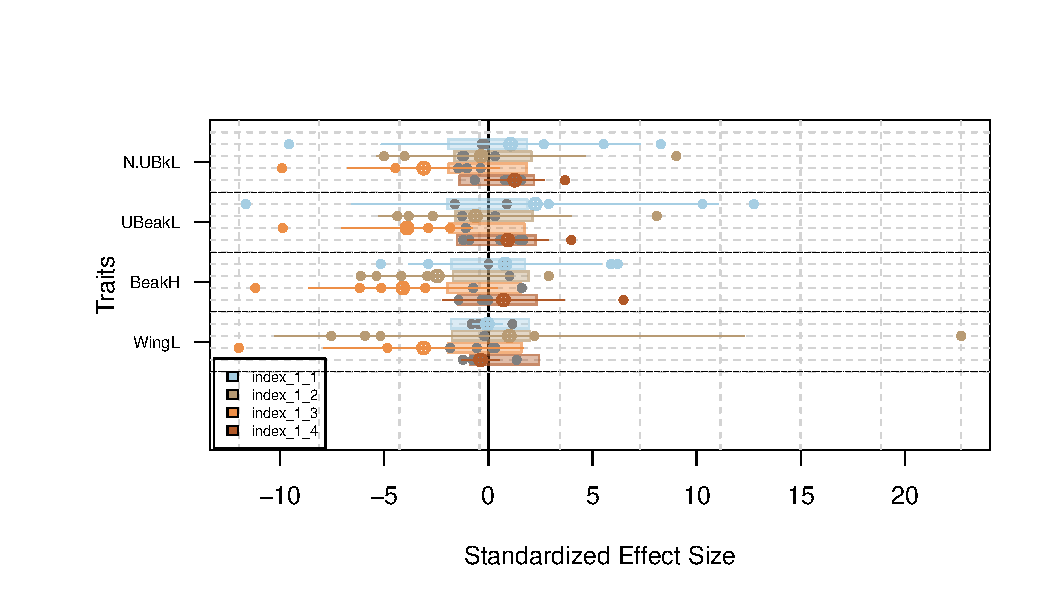
\includegraphics[width=\maxwidth]{figure/unnamed-chunk-46-1} 

}


\begin{kframe}\begin{alltt}
\hlkwd{plot}\hlstd{(res.finch.withoutIV)}
\end{alltt}
\end{kframe}

{\centering 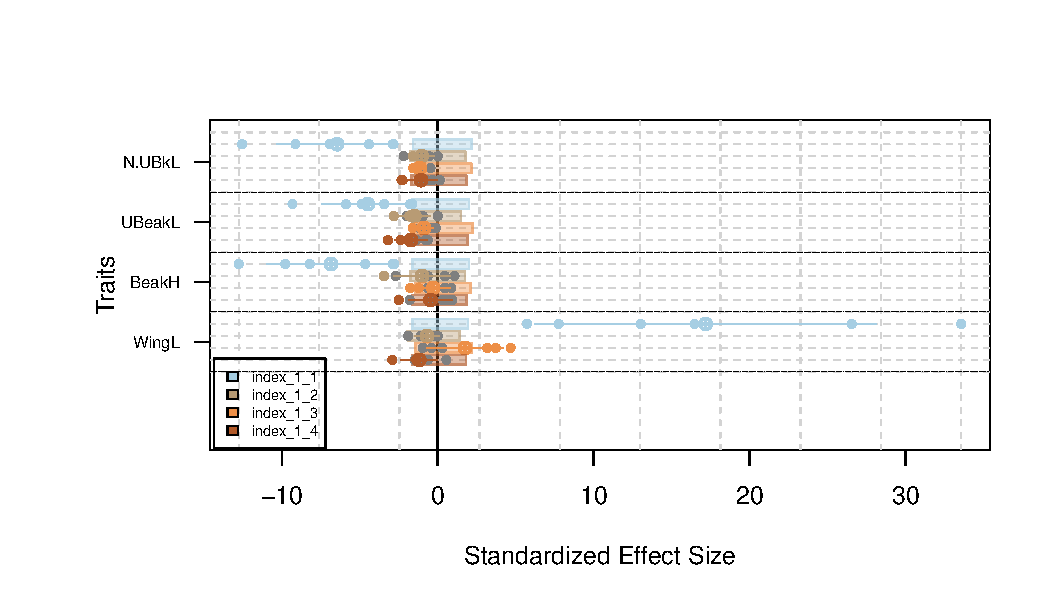
\includegraphics[width=\maxwidth]{figure/unnamed-chunk-46-2} 

}



\end{knitrout}
Now plot the two analysis together.

\begin{knitrout}
\definecolor{shadecolor}{rgb}{0.969, 0.969, 0.969}\color{fgcolor}\begin{kframe}
\begin{alltt}
\hlkwd{plot}\hlstd{(}\hlkwd{as.listofindex}\hlstd{(}\hlkwd{list}\hlstd{(res.finch.withIV, res.finch.withoutIV)))}
\end{alltt}
\end{kframe}
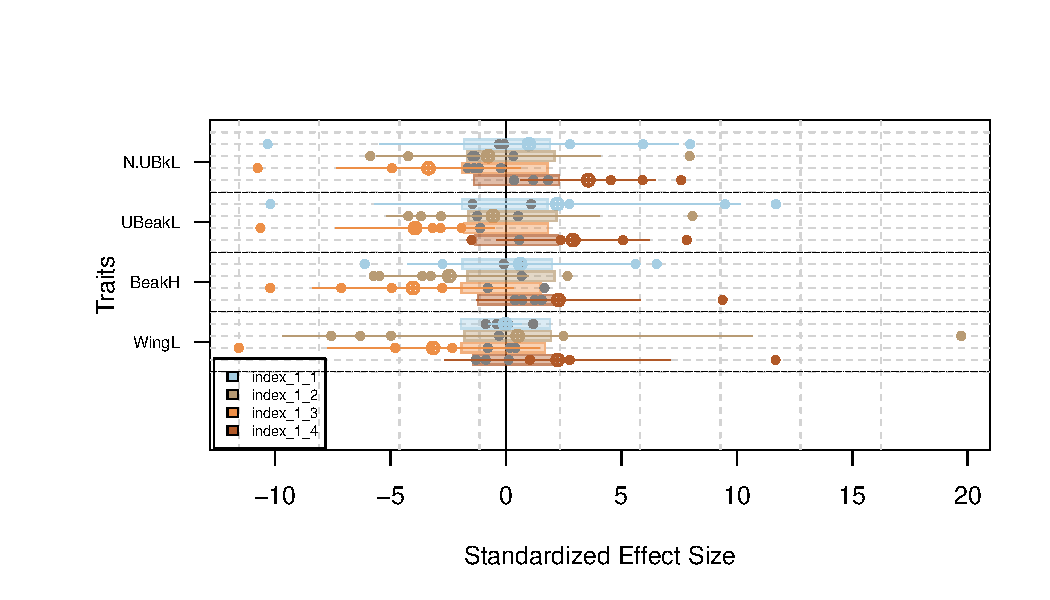
\includegraphics[width=\maxwidth]{figure/unnamed-chunk-47-1} 

\end{knitrout}

\subsubsection{Plot Tstats and other uni/multivariates metrics together}
The class listofindex permits to stock different metrics computed using \texttt{Tstats}, \texttt{ComIndex} and \texttt{ComIndexMulti} and compared to different null model. To do that we can use the Standardized Effect Size (ses) define as : 

\begin{center}
$SES = (I_obs – I_sim) / \delta_{sim}$
\end{center}

where $I_obs$ is the observed value, $I_sim$ the mean of values calculated from the null model and $\delta_{sim}$ the standard deviation of these simulated values.


\begin{knitrout}
\definecolor{shadecolor}{rgb}{0.969, 0.969, 0.969}\color{fgcolor}\begin{kframe}
\begin{alltt}
\hlstd{list.ind1}\hlkwb{<-}\hlkwd{list}\hlstd{(res.finch.withIV, res.finch.withoutIV)}
\hlstd{index.list1}\hlkwb{<-}\hlkwd{as.listofindex}\hlstd{(list.ind1)}

\hlkwd{plot}\hlstd{(index.list1)}
\end{alltt}
\end{kframe}
\end{knitrout}

\begin{knitrout}
\definecolor{shadecolor}{rgb}{0.969, 0.969, 0.969}\color{fgcolor}\begin{kframe}
\begin{alltt}
\hlstd{list.ind}\hlkwb{<-}\hlkwd{list}\hlstd{(res.finch.withIV, res.finch.withoutIV, res.finch)}
\hlstd{namesindex.i.l1} \hlkwb{=} \hlkwd{c}\hlstd{(}\hlstr{"mean"}\hlstd{,} \hlstr{"kurtosis"}\hlstd{,} \hlstr{"range"}\hlstd{,} \hlstr{"CVNND"}\hlstd{,}
         \hlstr{"mean.pop"}\hlstd{,} \hlstr{"kurtosis.pop"}\hlstd{,} \hlstr{"range.pop"}\hlstd{,} \hlstr{"CVNND.pop"}\hlstd{,}
         \hlstr{"T_IP.IC"}\hlstd{,} \hlstr{"T_IC.IR"}\hlstd{,} \hlstr{"T_PC.PR"}\hlstd{)}

\hlstd{i.l1}\hlkwb{<-}\hlkwd{as.listofindex}\hlstd{(list.ind,} \hlkwc{namesindex} \hlstd{= namesindex.i.l1)}

\hlkwd{class}\hlstd{(i.l1)}
\end{alltt}
\begin{verbatim}
## [1] "listofindex"
\end{verbatim}
\end{kframe}
\end{knitrout}

The plot type \texttt{bytraits} allows plotting all SES traits values for all sites or all traits
\begin{knitrout}
\definecolor{shadecolor}{rgb}{0.969, 0.969, 0.969}\color{fgcolor}\begin{kframe}
\begin{alltt}
\hlkwd{par}\hlstd{(}\hlkwc{mfrow} \hlstd{=} \hlkwd{c}\hlstd{(}\hlnum{2}\hlstd{,}\hlnum{3}\hlstd{))}
\hlkwd{plot}\hlstd{(i.l1,}\hlkwc{type} \hlstd{=} \hlstr{"bysites"}\hlstd{)}
\end{alltt}
\end{kframe}
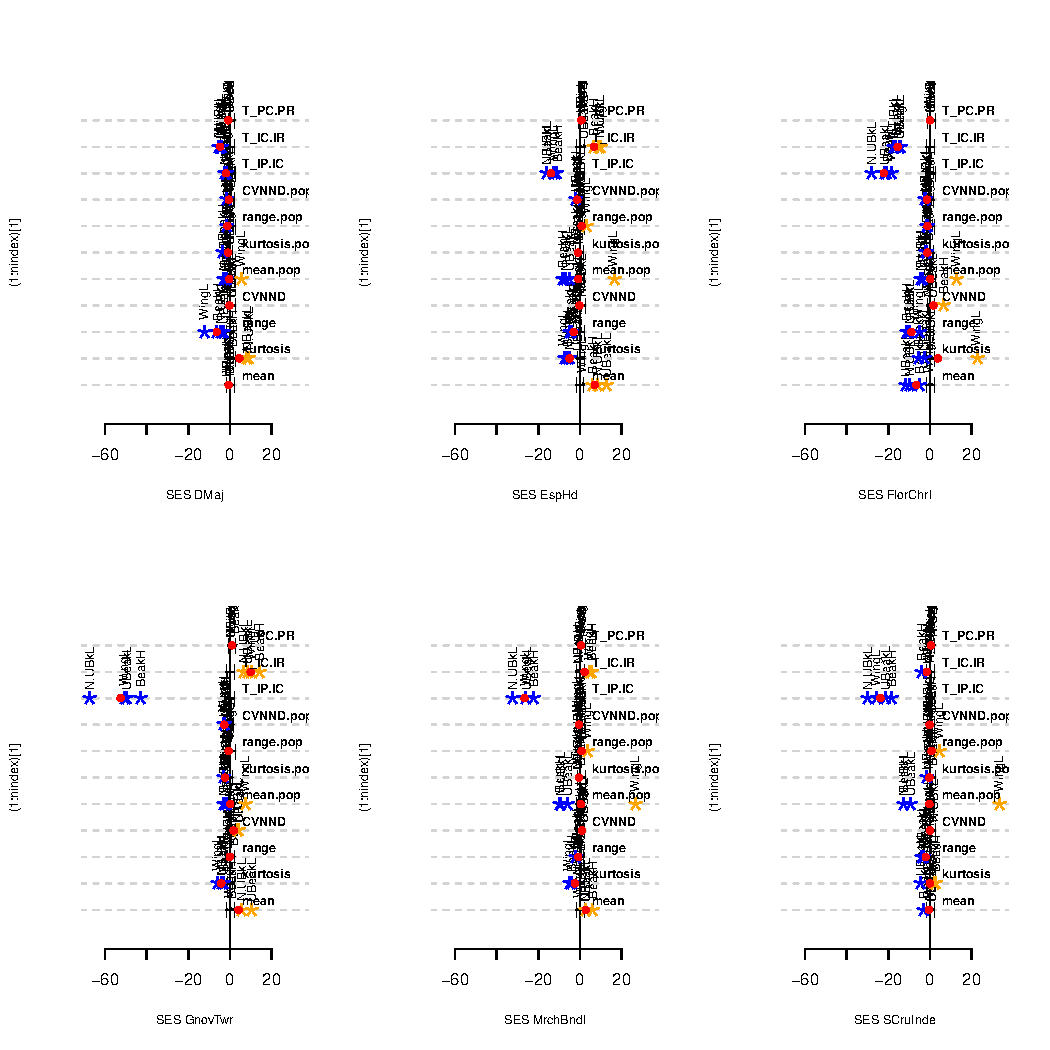
\includegraphics[width=\maxwidth]{figure/unnamed-chunk-50-1} 
\begin{kframe}\begin{alltt}
\hlkwd{par}\hlstd{(}\hlkwc{mfrow} \hlstd{=} \hlkwd{c}\hlstd{(}\hlnum{2}\hlstd{,}\hlnum{2}\hlstd{))}
\hlkwd{plot}\hlstd{(i.l1,}\hlkwc{type} \hlstd{=} \hlstr{"bytraits"}\hlstd{)}
\end{alltt}
\end{kframe}
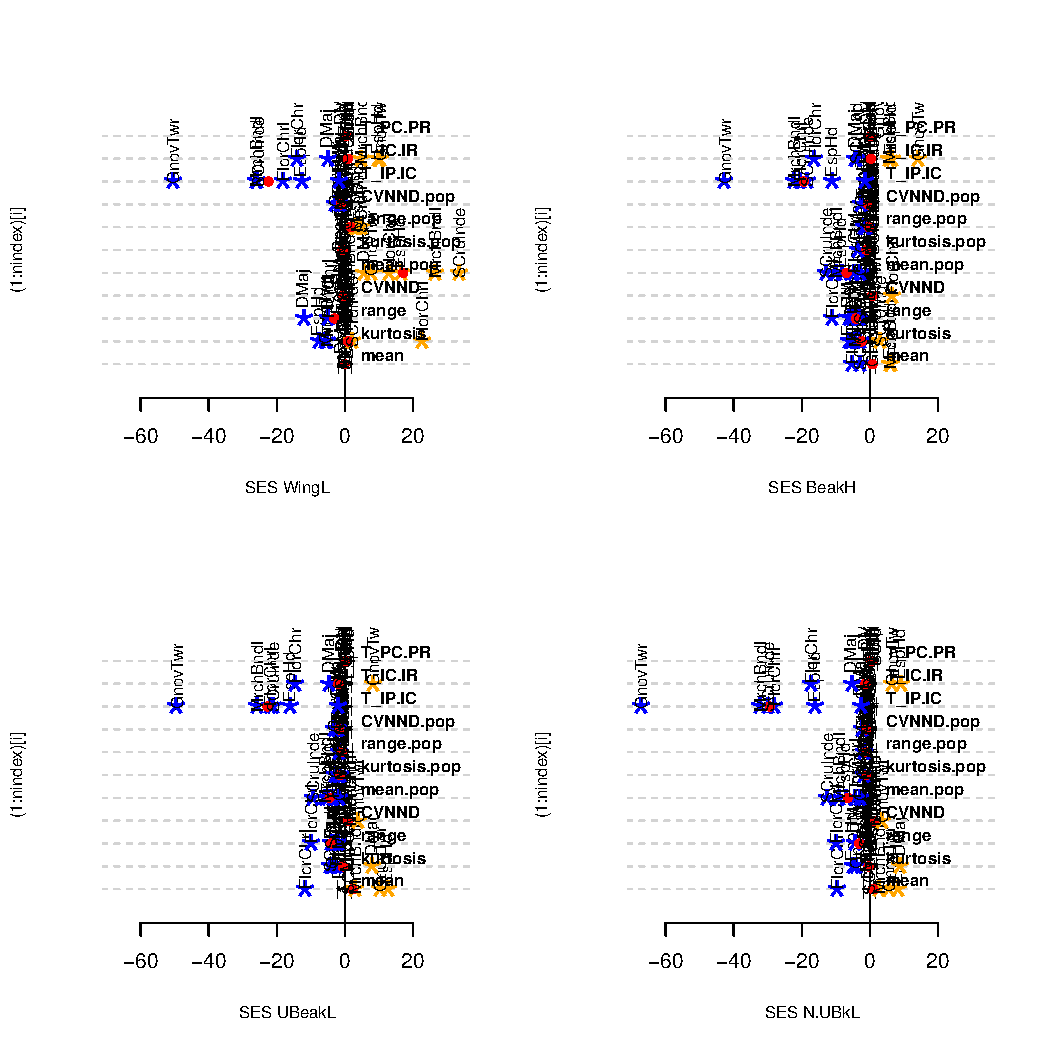
\includegraphics[width=\maxwidth]{figure/unnamed-chunk-50-2} 
\begin{kframe}\begin{alltt}
\hlkwd{par}\hlstd{(}\hlkwc{mfrow} \hlstd{=} \hlkwd{c}\hlstd{(}\hlnum{1}\hlstd{,}\hlnum{1}\hlstd{))}
\end{alltt}
\end{kframe}
\end{knitrout}

The other plot types are the same as plot.Tstats.

\begin{knitrout}
\definecolor{shadecolor}{rgb}{0.969, 0.969, 0.969}\color{fgcolor}\begin{kframe}
\begin{alltt}
\hlkwd{par}\hlstd{(}\hlkwc{mfrow} \hlstd{=} \hlkwd{c}\hlstd{(}\hlnum{2}\hlstd{,}\hlnum{2}\hlstd{))}

\hlkwd{plot}\hlstd{(i.l1)}
\hlkwd{plot}\hlstd{(i.l1,}\hlkwc{type} \hlstd{=} \hlstr{"simple_range"}\hlstd{)}
\hlkwd{plot}\hlstd{(i.l1,}\hlkwc{type} \hlstd{=} \hlstr{"normal"}\hlstd{)}
\hlkwd{plot}\hlstd{(i.l1,}\hlkwc{type} \hlstd{=} \hlstr{"barplot"}\hlstd{)}
\end{alltt}
\end{kframe}
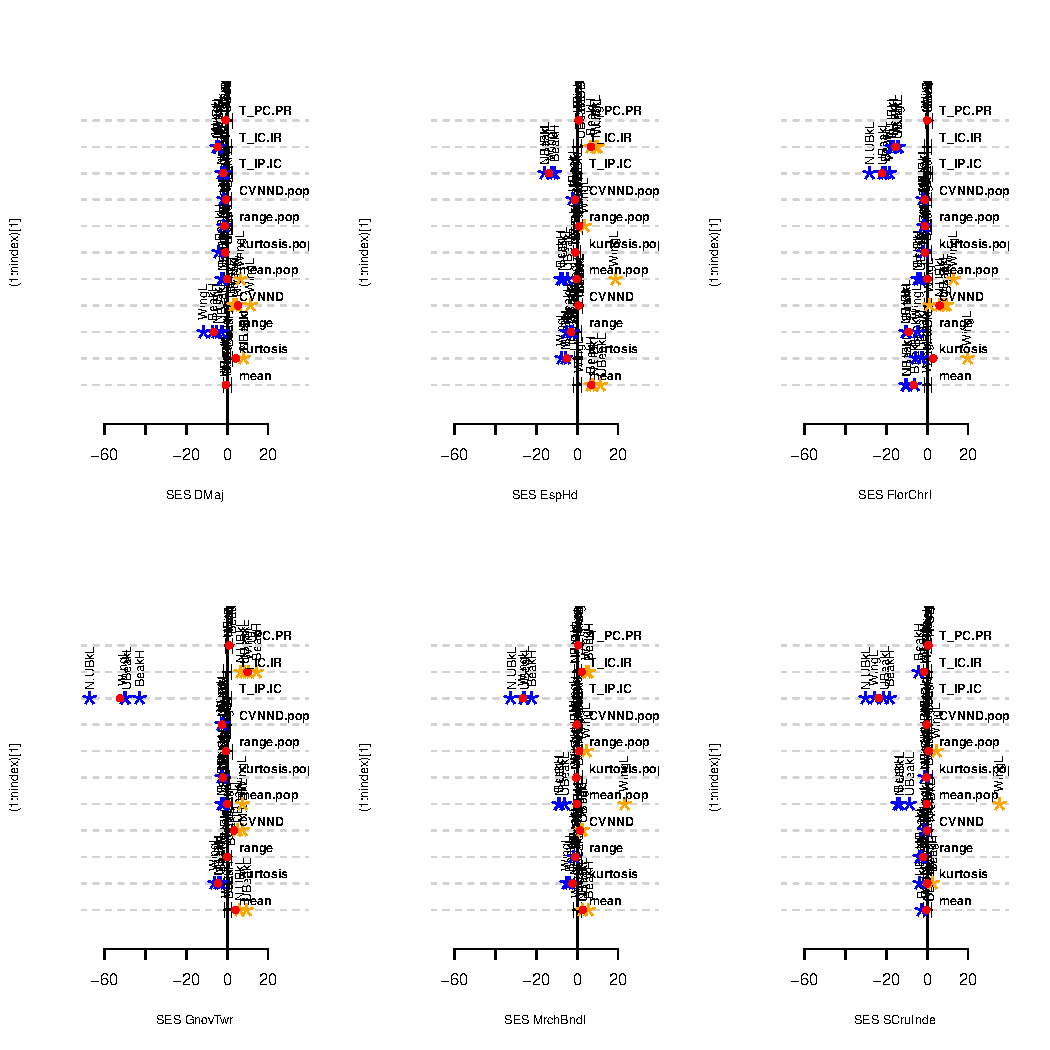
\includegraphics[width=\maxwidth]{figure/unnamed-chunk-51-1} 
\begin{kframe}\begin{alltt}
\hlkwd{par}\hlstd{(}\hlkwc{mfrow} \hlstd{=} \hlkwd{c}\hlstd{(}\hlnum{1}\hlstd{,}\hlnum{1}\hlstd{))}
\end{alltt}
\end{kframe}
\end{knitrout}



\newpage

\subsection{More information on multivariates index}

For most multivariate functions we need to replace (or exclude) NA values. For this example, we use the package \texttt{mice} to complete the data.

\begin{knitrout}
\definecolor{shadecolor}{rgb}{0.969, 0.969, 0.969}\color{fgcolor}\begin{kframe}
\begin{alltt}
\hlstd{comm}\hlkwb{<-}\hlkwd{t}\hlstd{(}\hlkwd{table}\hlstd{(ind.plot.finch,}\hlnum{1}\hlopt{:}\hlkwd{length}\hlstd{(ind.plot.finch)))}

\hlkwd{require}\hlstd{(mice)}
\hlstd{traits} \hlkwb{=} \hlstd{traits.finch}
\hlstd{mice}\hlkwb{<-}\hlkwd{mice}\hlstd{(traits.finch)}
\hlstd{traits.finch.mice}\hlkwb{<-}\hlkwd{complete}\hlstd{(mice)}
\end{alltt}
\end{kframe}
\end{knitrout}

A simple example to illustrate the concept of the function \texttt{ComIndexMulti}

\begin{knitrout}
\definecolor{shadecolor}{rgb}{0.969, 0.969, 0.969}\color{fgcolor}\begin{kframe}
\begin{alltt}
\hlstd{n_sp_plot}\hlkwb{<-}\hlkwd{as.factor}\hlstd{(}\hlkwd{paste}\hlstd{(sp.finch, ind.plot.finch,} \hlkwc{sep} \hlstd{=} \hlstr{"_"}\hlstd{))}
\hlstd{res.sum.1}\hlkwb{<-}\hlkwd{ComIndexMulti}\hlstd{(traits.finch,}
              \hlkwc{index} \hlstd{=} \hlkwd{c}\hlstd{(}\hlstr{"sum(scale(x), na.rm = T)"}\hlstd{,} \hlstr{"sum(x, na.rm = T)"}\hlstd{),}
              \hlkwc{by.factor} \hlstd{= n_sp_plot,} \hlkwc{nullmodels} \hlstd{=} \hlstr{"regional.ind"}\hlstd{,}
              \hlkwc{ind.plot} \hlstd{= ind.plot.finch,} \hlkwc{nperm} \hlstd{=} \hlnum{99}\hlstd{,} \hlkwc{sp} \hlstd{= sp.finch)}
\end{alltt}
\begin{verbatim}
## [1] "creating null models"
## [1] "regional.ind 25 %"
## [1] "regional.ind 50 %"
## [1] "regional.ind 75 %"
## [1] "regional.ind 100 %"
## [1] "calculation of null values using null models"
## [1] "sum(scale(x), na.rm = T) 50 %"
## [1] "sum(x, na.rm = T) 100 %"
## [1] "calculation of observed values"
## [1] "50 %"
## [1] "100 %"
\end{verbatim}
\begin{alltt}
\hlstd{res.sum.1}
\end{alltt}
\begin{verbatim}
## 	#################################
## 	# Community metrics calculation #
## 	#################################
## class: ComIndexMulti
## $call: ComIndexMulti(traits = traits.finch, index = c("sum(scale(x), na.rm = T)", 
##     "sum(x, na.rm = T)"), by.factor = n_sp_plot, nullmodels = "regional.ind", 
##     ind.plot = ind.plot.finch, sp = sp.finch, nperm = 99)
## 
## ###############
## $obs: list of observed values
## 	$sum(scale(x), na.rm = T)
## 	$sum(x, na.rm = T)
## 
## ###############
## $null: list of null values, number of permutation: NA 
## 	$sum(scale(x), na.rm = T)_nm ... null model = regional.ind
## 	$sum(x, na.rm = T)_nm ... null model = regional.ind
## 
## ###############
## data used
##   data      class      dim   
## 1 $traits   data.frame 2513,4
## 2 $ind.plot factor     2513  
## 3 $sp       factor     2513  
##   content                                             
## 1 traits data                                         
## 2 name of the plot in which the individual is         
## 3 groups (e.g. species) which the individual belong to
## 
## ###############
## others
## 	$namestraits: 4 traits
## [1] "WingL"  "BeakH"  "UBeakL" "N.UBkL"
## 
## 	$sites_richness:
## 	    DMaj    EspHd FlorChrl  GnovTwr MrchBndl SCruInde 
##       50      267      981      258      270      687
\end{verbatim}
\end{kframe}
\end{knitrout}

\newpage
A more interesting example using the function \texttt{hypervolume} from the package ... \texttt{hypervolume} (Blonder et al., 2014). We show here several results which differed in there factor that delimit the group to calculate different hypervolume (argument \texttt{byfactor}). 

First, let's try the \texttt{hypervolume} function one finch data.
\begin{knitrout}
\definecolor{shadecolor}{rgb}{0.969, 0.969, 0.969}\color{fgcolor}\begin{kframe}
\begin{alltt}
\hlstd{hv}\hlkwb{<-}\hlkwd{hypervolume}\hlstd{(traits.finch.mice,} \hlkwc{reps} \hlstd{=} \hlnum{100}\hlstd{,}
                \hlkwc{bandwidth} \hlstd{=} \hlnum{0.2}\hlstd{,} \hlkwc{verbose} \hlstd{= F,} \hlkwc{warnings} \hlstd{= F)}
\hlkwd{plot}\hlstd{(hv)}
\end{alltt}
\begin{verbatim}
## Showing 1000 random points of 129088 for untitled
## Showing 1000 data points of 2513 for untitled
\end{verbatim}
\end{kframe}
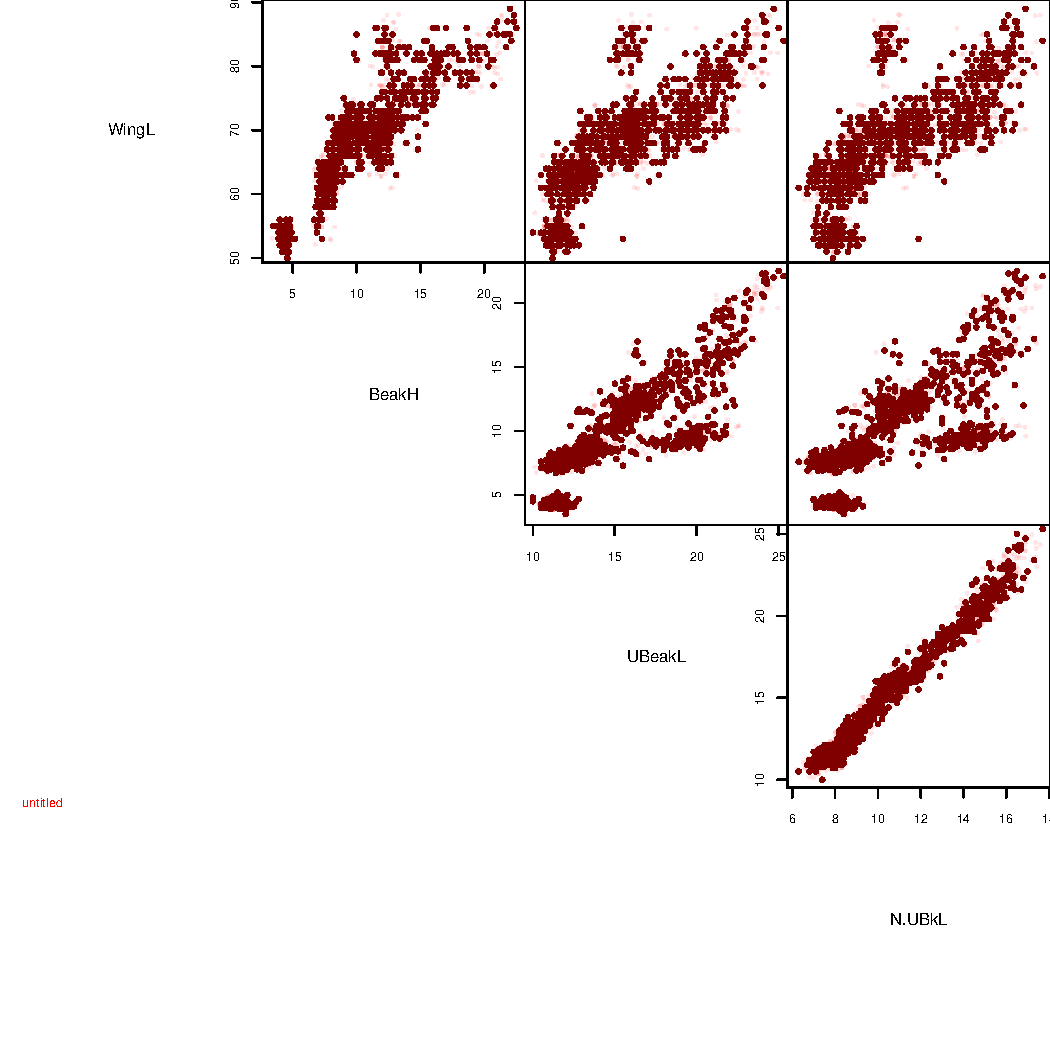
\includegraphics[width=\maxwidth]{figure/unnamed-chunk-54-1} 

\end{knitrout}

Now, we can do the same analysis for each species.

\begin{knitrout}
\definecolor{shadecolor}{rgb}{0.969, 0.969, 0.969}\color{fgcolor}\begin{kframe}
\begin{alltt}
\hlstd{hv.list}\hlkwb{<-}\hlkwd{new}\hlstd{(}\hlstr{"HypervolumeList"}\hlstd{)}
\hlstd{hv.list2}\hlkwb{<-}\hlkwd{list}\hlstd{()}

\hlkwa{for}\hlstd{(i} \hlkwa{in} \hlnum{1}\hlopt{:} \hlkwd{length}\hlstd{(}\hlkwd{table}\hlstd{(sp.finch))) \{}
 \hlstd{hv.list2[[i]]}\hlkwb{<-}\hlkwd{hypervolume}\hlstd{(traits.finch.mice[sp.finch} \hlopt{==} \hlkwd{levels}\hlstd{(sp.finch)[i], ],}
        \hlkwc{reps} \hlstd{=} \hlnum{1000}\hlstd{,}\hlkwc{bandwidth} \hlstd{=} \hlnum{0.2}\hlstd{,} \hlkwc{verbose} \hlstd{= F,} \hlkwc{warnings} \hlstd{= F)}
\hlstd{\}}

\hlstd{hv.list}\hlopt{@}\hlkwc{HVList}\hlkwb{<-}\hlstd{hv.list2}
\hlkwd{require}\hlstd{(adegenet)}
\end{alltt}


{\ttfamily\noindent\itshape\color{messagecolor}{\#\# Loading required package: adegenet\\\#\#\ \ \ \ ==========================\\\#\#\ \ \ \  adegenet 1.4-2 is loaded\\\#\#\ \ \ \ ==========================\\\#\# \\\#\#\ \ - to start, type '?adegenet'\\\#\#\ \ - to browse adegenet website, type 'adegenetWeb()'\\\#\#\ \ - to post questions/comments: adegenet-forum@lists.r-forge.r-project.org}}\begin{alltt}
\hlstd{colorhv}\hlkwb{<-}\hlkwd{transp}\hlstd{(}\hlkwd{funky}\hlstd{(}\hlkwd{nlevels}\hlstd{(sp.finch)),} \hlkwc{alpha} \hlstd{=} \hlnum{0.8}\hlstd{)}

\hlkwd{plot}\hlstd{(hv.list,} \hlkwc{colors} \hlstd{= colorhv,} \hlkwc{darkfactor} \hlstd{=} \hlnum{0.8}\hlstd{)}
\end{alltt}
\end{kframe}
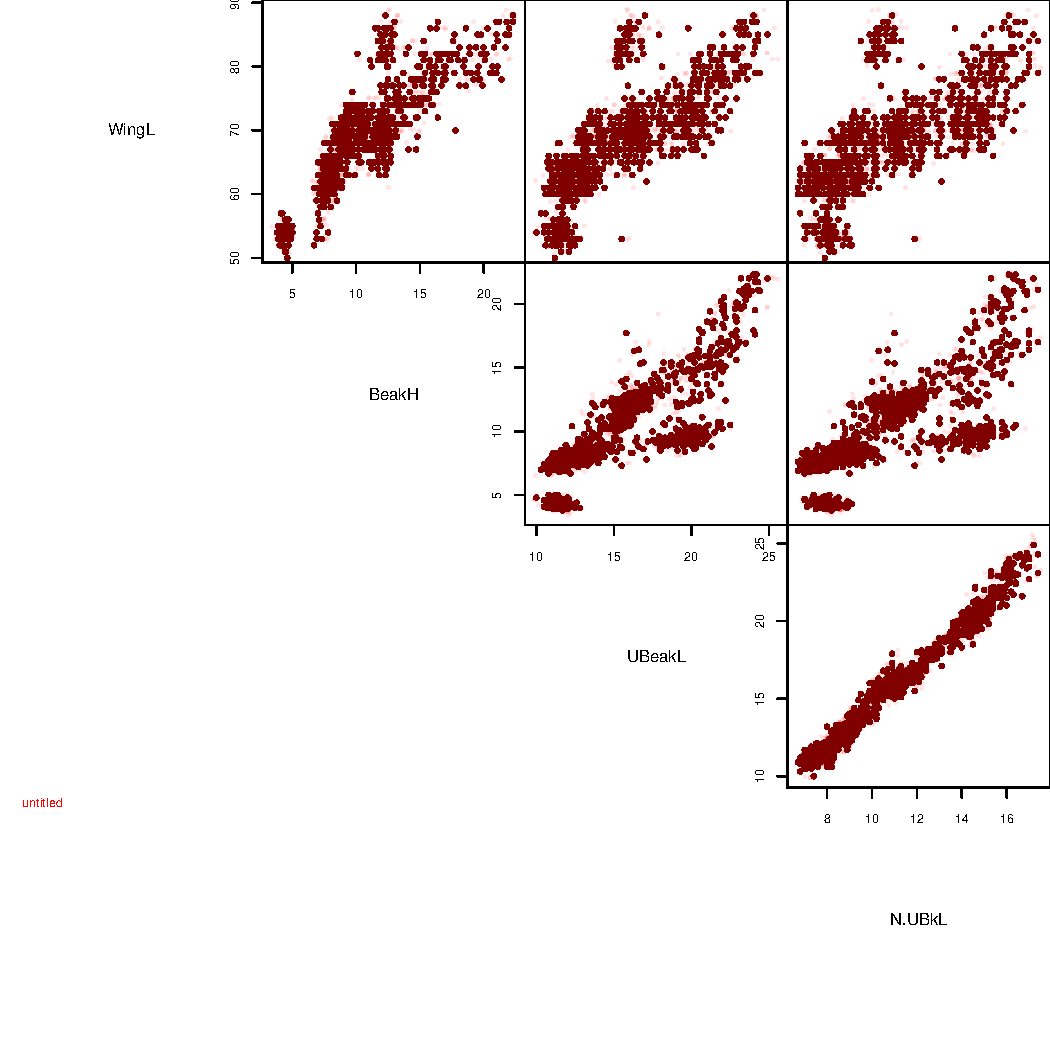
\includegraphics[width=\maxwidth]{figure/unnamed-chunk-55-1} 
\begin{kframe}\begin{alltt}
\hlkwd{plot}\hlstd{(hv.list,} \hlkwc{colors} \hlstd{= colorhv,} \hlkwc{darkfactor} \hlstd{=} \hlnum{0.8}\hlstd{,} \hlkwc{showdata} \hlstd{= F,}
     \hlkwc{npmax_random} \hlstd{=} \hlnum{200}\hlstd{,} \hlkwc{cex.random} \hlstd{=} \hlnum{1}\hlstd{)}
\end{alltt}
\end{kframe}
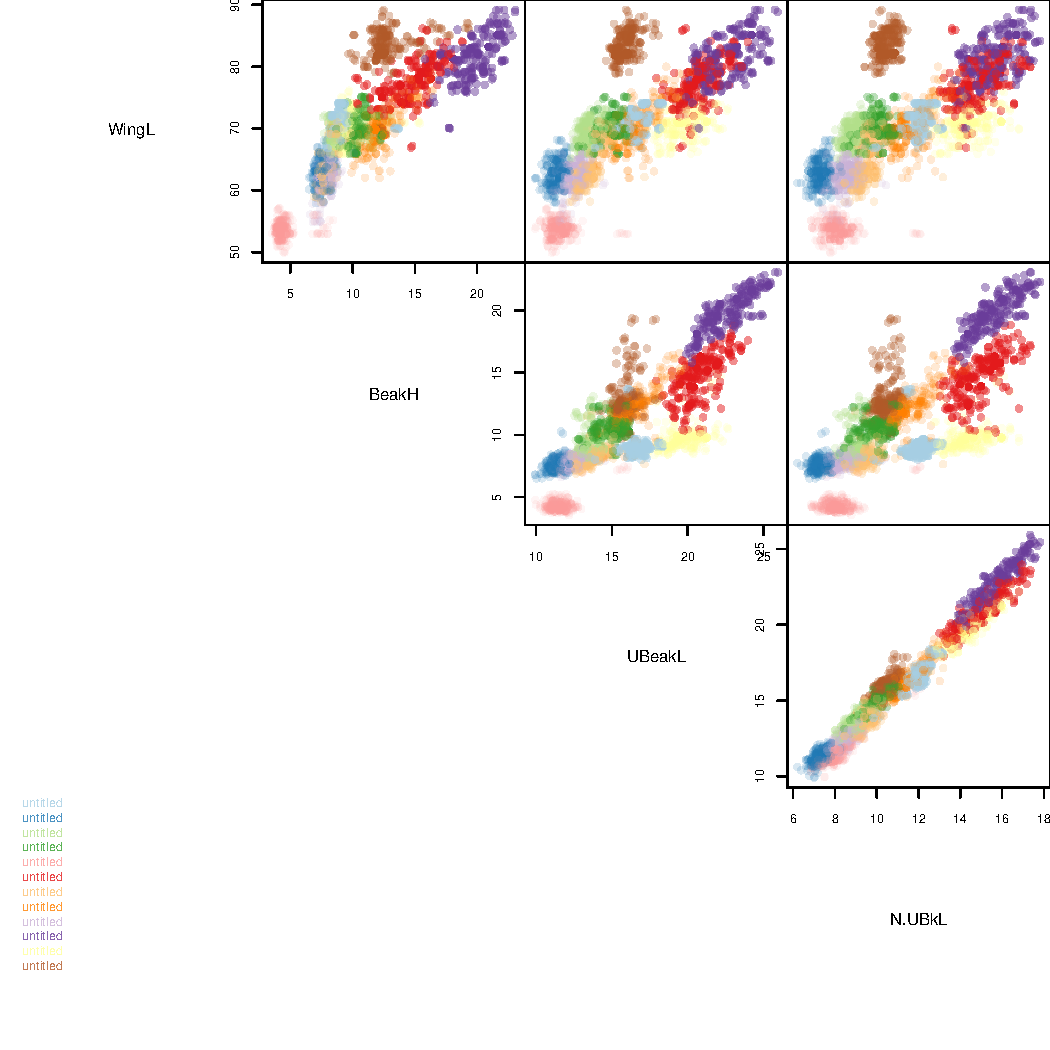
\includegraphics[width=\maxwidth]{figure/unnamed-chunk-55-2} 

\end{knitrout}

\begin{knitrout}
\definecolor{shadecolor}{rgb}{0.969, 0.969, 0.969}\color{fgcolor}\begin{kframe}
\begin{alltt}
\hlkwd{summary}\hlstd{(hv.list)}
\end{alltt}
\end{kframe}
\end{knitrout}

The standard example of the \texttt{hypervolume} package also use finch data but at the species level.

\begin{knitrout}
\definecolor{shadecolor}{rgb}{0.969, 0.969, 0.969}\color{fgcolor}\begin{kframe}
\begin{alltt}
\hlstd{doHypervolumeFinchDemo}\hlkwb{=}\hlnum{TRUE}
\hlkwd{demo}\hlstd{(}\hlstr{'finch'}\hlstd{,} \hlkwc{package} \hlstd{=} \hlstr{'hypervolume'}\hlstd{)}
\end{alltt}
\end{kframe}
\end{knitrout}


\texttt{ComIndexMulti} takes the same arguments as \texttt{ComIndex} and an argument by factor to apply the index on different factors.
\label{hv.3}
\begin{knitrout}
\definecolor{shadecolor}{rgb}{0.969, 0.969, 0.969}\color{fgcolor}\begin{kframe}
\begin{alltt}
\hlcom{#all individual are put in the same group: calculate the hypervolume without by.factor}
\hlstd{hv.1}\hlkwb{<-}\hlkwd{ComIndexMulti}\hlstd{(traits.finch.mice,}
             \hlkwc{index} \hlstd{=} \hlkwd{c}\hlstd{(}\hlstr{"as.numeric(try(hypervolume(na.omit(x), reps = 100,
                       bandwidth = 0.2, verbose = F, warnings = F)@Volume))"}\hlstd{),}
             \hlkwc{by.factor} \hlstd{=} \hlkwd{rep}\hlstd{(}\hlnum{1}\hlstd{,}\hlkwd{length}\hlstd{(n_sp_plot)),} \hlkwc{nullmodels} \hlstd{=} \hlstr{"regional.ind"}\hlstd{,}
             \hlkwc{ind.plot} \hlstd{= ind.plot.finch,} \hlkwc{nperm} \hlstd{=} \hlnum{99}\hlstd{,} \hlkwc{sp} \hlstd{= sp.finch)}
\end{alltt}
\begin{verbatim}
## [1] "creating null models"
## [1] "regional.ind 25 %"
## [1] "regional.ind 50 %"
## [1] "regional.ind 75 %"
## [1] "regional.ind 100 %"
## [1] "calculation of null values using null models"
## [1] "as.numeric(try(hypervolume(na.omit(x), reps = 100,\n                       bandwidth = 0.2, verbose = F, warnings = F)@Volume)) 100 %"
## [1] "calculation of observed values"
## [1] "100 %"
\end{verbatim}
\begin{alltt}
\hlstd{hv.2}\hlkwb{<-}\hlkwd{ComIndexMulti}\hlstd{(traits.finch.mice,}
             \hlkwc{index} \hlstd{=} \hlkwd{c}\hlstd{(}\hlstr{"as.numeric(try(hypervolume(na.omit(x), reps = 100,
                       bandwidth = 0.2, verbose = F, warnings = F)@Volume))"}\hlstd{),}
             \hlkwc{by.factor} \hlstd{= n_sp_plot,} \hlkwc{nullmodels} \hlstd{=} \hlstr{"regional.ind"}\hlstd{,}
             \hlkwc{ind.plot} \hlstd{= ind.plot.finch,} \hlkwc{nperm} \hlstd{=} \hlnum{99}\hlstd{,} \hlkwc{sp} \hlstd{= sp.finch,} \hlkwc{print} \hlstd{=} \hlnum{FALSE}\hlstd{)}

\hlstd{ptm} \hlkwb{<-} \hlkwd{proc.time}\hlstd{()}
\hlstd{hv.3}\hlkwb{<-}\hlkwd{ComIndexMulti}\hlstd{(traits.finch.mice,}
             \hlkwc{index} \hlstd{=} \hlkwd{c}\hlstd{(}\hlstr{"as.numeric(try(hypervolume(na.omit(x), reps = 100,
                       bandwidth = 0.2, verbose = F, warnings = F)@Volume))"}\hlstd{),}
             \hlkwc{by.factor} \hlstd{= ind.plot.finch,} \hlkwc{nullmodels} \hlstd{=}\hlstr{"regional.ind"}\hlstd{,}
             \hlkwc{ind.plot} \hlstd{= ind.plot.finch,} \hlkwc{nperm} \hlstd{=} \hlnum{99}\hlstd{,} \hlkwc{sp} \hlstd{= sp.finch,} \hlkwc{print} \hlstd{=} \hlnum{FALSE}\hlstd{)}
\hlstd{proc.time_ComIndexMulti} \hlkwb{<-} \hlkwd{proc.time}\hlstd{()} \hlopt{-} \hlstd{ptm}

\hlstd{hv.4}\hlkwb{<-}\hlkwd{ComIndexMulti}\hlstd{(traits.finch.mice,}
             \hlkwc{index} \hlstd{=} \hlkwd{c}\hlstd{(}\hlstr{"as.numeric(try(hypervolume(na.omit(x), reps = 100, 
                       bandwidth = 0.2, verbose = F, warnings = F)@Volume))"}\hlstd{),}
             \hlkwc{by.factor} \hlstd{= sp.finch,} \hlkwc{nullmodels} \hlstd{=} \hlstr{"regional.ind"}\hlstd{,}
             \hlkwc{ind.plot} \hlstd{= ind.plot.finch,} \hlkwc{nperm} \hlstd{=} \hlnum{99}\hlstd{,} \hlkwc{sp} \hlstd{= sp.finch,} \hlkwc{print} \hlstd{=} \hlnum{FALSE}\hlstd{)}

\hlstd{list.ind.multi}\hlkwb{<-}\hlkwd{as.listofindex}\hlstd{(}\hlkwd{list}\hlstd{(hv.2, hv.3, hv.4))}

\hlstd{ses.list.multi}\hlkwb{<-}\hlkwd{ses.listofindex}\hlstd{(list.ind.multi)}
\end{alltt}
\end{kframe}
\end{knitrout}

\begin{knitrout}
\definecolor{shadecolor}{rgb}{0.969, 0.969, 0.969}\color{fgcolor}\begin{kframe}
\begin{alltt}
\hlkwd{plot}\hlstd{(list.ind.multi)}
\end{alltt}
\end{kframe}

{\centering 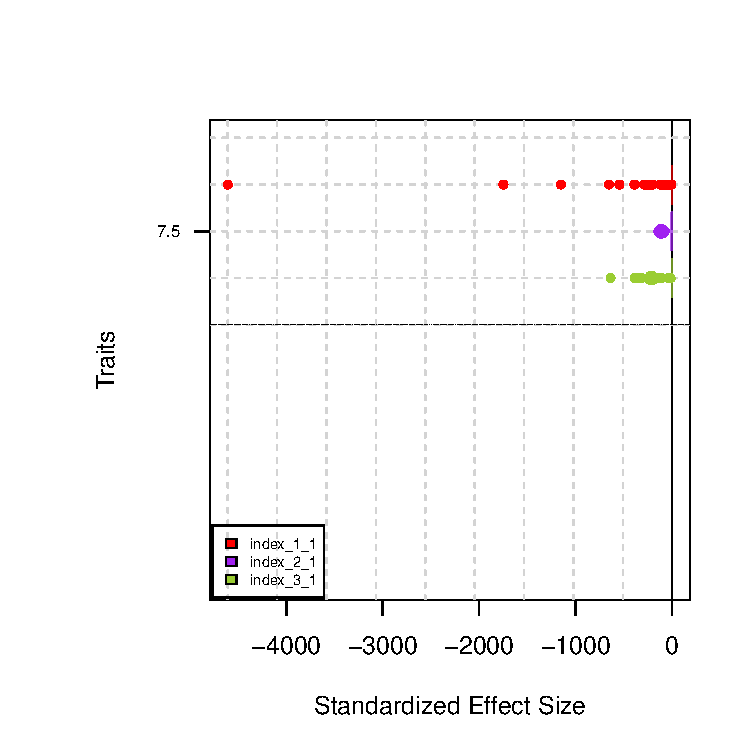
\includegraphics[width=\maxwidth]{figure/unnamed-chunk-59-1} 

}


\begin{kframe}\begin{alltt}
\hlcom{#Try a zoom on the area near zero}
\hlkwd{plot}\hlstd{(list.ind.multi,} \hlkwc{xlim} \hlstd{=} \hlkwd{c}\hlstd{(}\hlopt{-}\hlnum{200}\hlstd{,}\hlnum{20}\hlstd{))}
\end{alltt}
\end{kframe}

{\centering 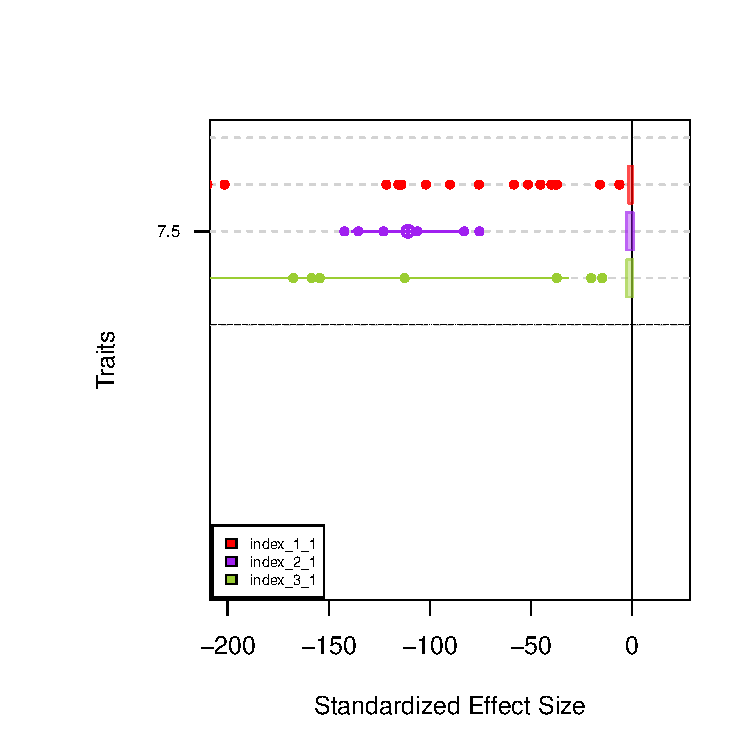
\includegraphics[width=\maxwidth]{figure/unnamed-chunk-59-2} 

}



\end{knitrout}

Compare hypervolume to Villeger's metrics convex hull.

\begin{knitrout}
\definecolor{shadecolor}{rgb}{0.969, 0.969, 0.969}\color{fgcolor}\begin{kframe}
\begin{alltt}
\hlkwd{require}\hlstd{(}\hlstr{"geometry"}\hlstd{)}
\end{alltt}


{\ttfamily\noindent\itshape\color{messagecolor}{\#\# Loading required package: geometry\\\#\# Loading required package: magic\\\#\# Loading required package: abind}}\begin{alltt}
\hlstd{FA}\hlkwb{<-}\hlkwd{as.character}\hlstd{(}\hlstr{"FA"}\hlstd{)}
\hlstd{funct}\hlkwb{<-}\hlkwd{c}\hlstd{(}\hlstr{"round(convhulln(x,FA)$vol,6)"}\hlstd{)}

\hlcom{##Null model local is trivial for this function}
\hlcom{##because randomization is within community only}
\hlstd{Fdis.finch}\hlkwb{<-}\hlkwd{ComIndexMulti}\hlstd{(traits.finch.mice,}
             \hlkwc{index} \hlstd{= funct,}
             \hlkwc{by.factor} \hlstd{= ind.plot.finch,} \hlkwc{nullmodels} \hlstd{=} \hlstr{"local"}\hlstd{,}
             \hlkwc{ind.plot} \hlstd{= ind.plot.finch,} \hlkwc{nperm} \hlstd{=} \hlnum{99}\hlstd{,} \hlkwc{sp} \hlstd{= sp.finch)}
\end{alltt}
\begin{verbatim}
## [1] "creating null models"
## [1] "local 25 %"
## [1] "local 50 %"
## [1] "local 75 %"
## [1] "local 100 %"
## [1] "calculation of null values using null models"
## [1] "round(convhulln(x,FA)$vol,6) 100 %"
## [1] "calculation of observed values"
## [1] "100 %"
\end{verbatim}
\begin{alltt}
\hlstd{list.ind.multi2}\hlkwb{<-}\hlkwd{as.listofindex}\hlstd{(}\hlkwd{list}\hlstd{(hv.3, Fdis.finch))}

\hlstd{ses.list.multi2}\hlkwb{<-}\hlkwd{ses.listofindex}\hlstd{(list.ind.multi2)}
\end{alltt}
\end{kframe}
\end{knitrout}

\begin{knitrout}
\definecolor{shadecolor}{rgb}{0.969, 0.969, 0.969}\color{fgcolor}\begin{kframe}
\begin{alltt}
\hlkwd{plot}\hlstd{(list.ind.multi2)}
\end{alltt}
\end{kframe}
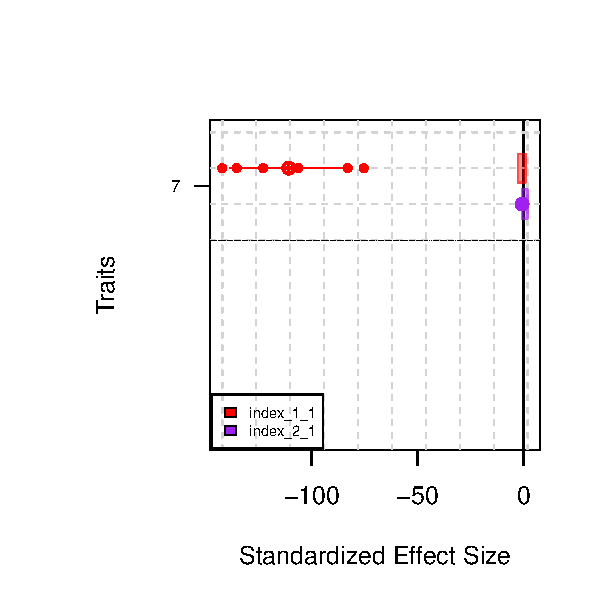
\includegraphics[width=\maxwidth]{figure/unnamed-chunk-61-1} 

\end{knitrout}

\section{Others graphical functions}

Use rasterVis to obtain more color schemes. 
\begin{knitrout}
\definecolor{shadecolor}{rgb}{0.969, 0.969, 0.969}\color{fgcolor}\begin{kframe}


{\ttfamily\noindent\itshape\color{messagecolor}{\#\# Loading required package: rasterVis\\\#\# Loading required package: raster\\\#\# Loading required package: sp\\\#\# \\\#\# Attaching package: 'raster'\\\#\# \\\#\# The following object is masked from 'package:magic':\\\#\# \\\#\#\ \ \ \  shift\\\#\# \\\#\# The following objects are masked from 'package:ape':\\\#\# \\\#\#\ \ \ \  rotate, zoom\\\#\# \\\#\# The following object is masked from 'package:nlme':\\\#\# \\\#\#\ \ \ \  getData\\\#\# \\\#\# Loading required package: latticeExtra\\\#\# Loading required package: RColorBrewer\\\#\# Loading required package: hexbin}}\end{kframe}
\end{knitrout}

Plot the p-value or the ses values using the function \texttt{levelplot}.

\begin{knitrout}
\definecolor{shadecolor}{rgb}{0.969, 0.969, 0.969}\color{fgcolor}\begin{kframe}
\begin{alltt}
\hlkwd{levelplot}\hlstd{(}\hlkwd{t}\hlstd{(}\hlkwd{sum_Tstats}\hlstd{(res.finch)}\hlopt{$}\hlstd{p.value),}
     \hlkwc{colorkey} \hlstd{= my.ckey,} \hlkwc{par.settings} \hlstd{= my.theme,}\hlkwc{border} \hlstd{=} \hlstr{"black"}\hlstd{)}
\end{alltt}
\end{kframe}
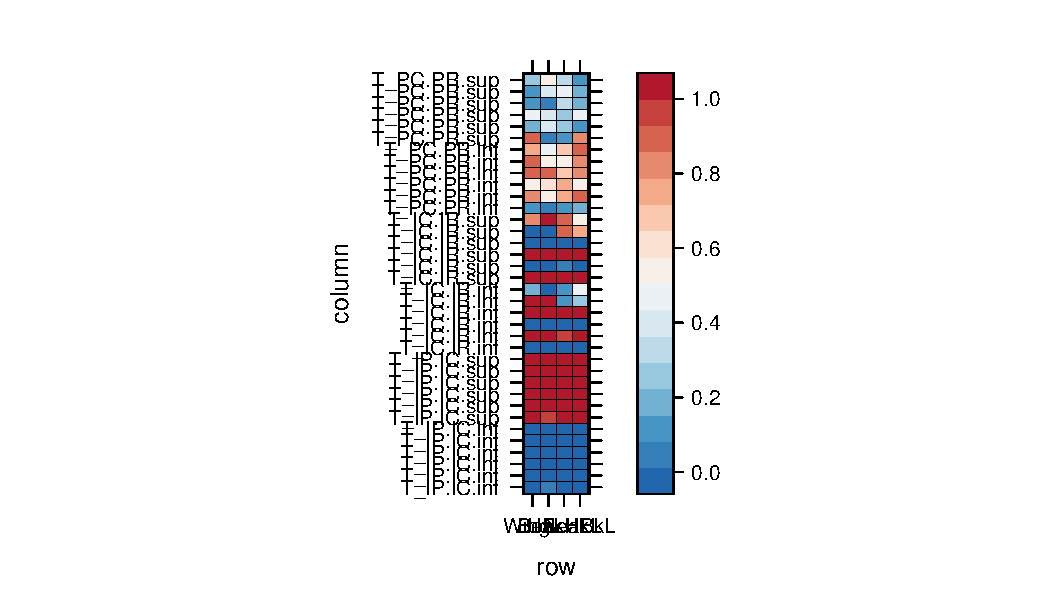
\includegraphics[width=\maxwidth]{figure/unnamed-chunk-63-1} 

\end{knitrout}


\begin{knitrout}
\definecolor{shadecolor}{rgb}{0.969, 0.969, 0.969}\color{fgcolor}\begin{kframe}
\begin{alltt}
\hlkwd{levelplot}\hlstd{(}\hlkwd{t}\hlstd{(}\hlkwd{ses}\hlstd{(res.finch}\hlopt{$}\hlstd{Tstats}\hlopt{$}\hlstd{T_IP.IC, res.finch}\hlopt{$}\hlstd{Tstats}\hlopt{$}\hlstd{T_IP.IC_nm)}\hlopt{$}\hlstd{ses),}
     \hlkwc{colorkey} \hlstd{= my.ckey,} \hlkwc{par.settings} \hlstd{= my.theme,}\hlkwc{border} \hlstd{=} \hlstr{"black"}\hlstd{)}
\end{alltt}
\end{kframe}
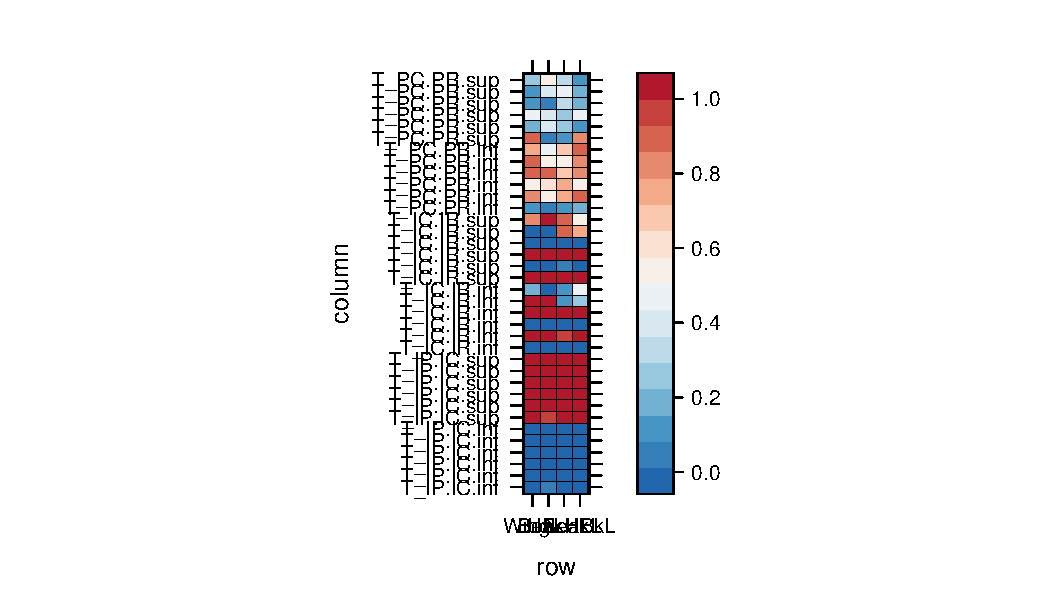
\includegraphics[width=\maxwidth]{figure/unnamed-chunk-64-1} 
\begin{kframe}\begin{alltt}
\hlkwd{levelplot}\hlstd{(}\hlkwd{cbind}\hlstd{(}\hlkwd{t}\hlstd{(}\hlkwd{ses}\hlstd{(res.finch}\hlopt{$}\hlstd{Tstats}\hlopt{$}\hlstd{T_IP.IC, res.finch}\hlopt{$}\hlstd{Tstats}\hlopt{$}\hlstd{T_IP.IC_nm)}\hlopt{$}\hlstd{ses),}
        \hlkwd{t}\hlstd{(}\hlkwd{ses}\hlstd{(res.finch}\hlopt{$}\hlstd{Tstats}\hlopt{$}\hlstd{T_IC.IR, res.finch}\hlopt{$}\hlstd{Tstats}\hlopt{$}\hlstd{T_IP.IC_nm)}\hlopt{$}\hlstd{ses),}
        \hlkwd{t}\hlstd{(}\hlkwd{ses}\hlstd{(res.finch}\hlopt{$}\hlstd{Tstats}\hlopt{$}\hlstd{T_PC.PR, res.finch}\hlopt{$}\hlstd{Tstats}\hlopt{$}\hlstd{T_IP.IC_nm)}\hlopt{$}\hlstd{ses))}
     \hlstd{,} \hlkwc{colorkey} \hlstd{= my.ckey,} \hlkwc{par.settings} \hlstd{= my.theme,}\hlkwc{border} \hlstd{=} \hlstr{"black"}\hlstd{)}
\end{alltt}
\end{kframe}
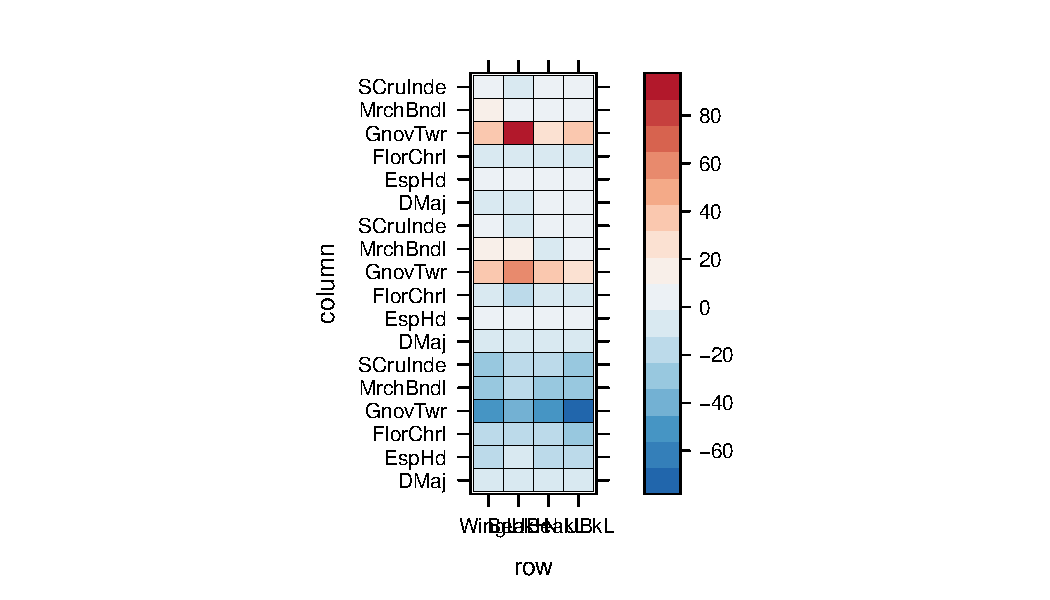
\includegraphics[width=\maxwidth]{figure/unnamed-chunk-64-2} 

\end{knitrout}

Another example using \texttt{ses.listofindex}. The first plot represent "ses" values and the second one the result of a test with H0: observed index value are greater than what we can expect using the null model (alpha = 2.5\%).

\begin{knitrout}
\definecolor{shadecolor}{rgb}{0.969, 0.969, 0.969}\color{fgcolor}\begin{kframe}
\begin{alltt}
\hlstd{ses.list}\hlkwb{<-}\hlkwd{ses.listofindex}\hlstd{(i.l1)}

\hlkwd{levelplot}\hlstd{(}\hlkwd{t}\hlstd{(}\hlkwd{rbind}\hlstd{(ses.list[[}\hlnum{1}\hlstd{]]}\hlopt{$}\hlstd{ses, ses.list[[}\hlnum{2}\hlstd{]]}\hlopt{$}\hlstd{ses,}
         \hlstd{ses.list[[}\hlnum{3}\hlstd{]]}\hlopt{$}\hlstd{ses, ses.list[[}\hlnum{4}\hlstd{]]}\hlopt{$}\hlstd{ses)),}
     \hlkwc{colorkey} \hlstd{= my.ckey,} \hlkwc{par.settings} \hlstd{= my.theme,}\hlkwc{border} \hlstd{=} \hlstr{"black"}\hlstd{)}
\end{alltt}
\end{kframe}
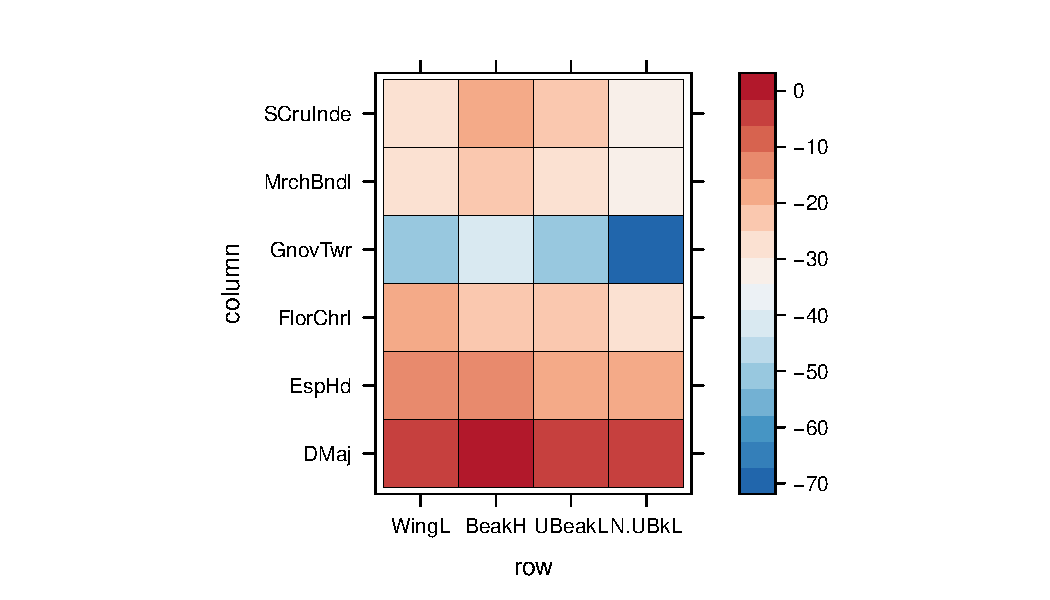
\includegraphics[width=\maxwidth]{figure/unnamed-chunk-65-1} 
\begin{kframe}\begin{alltt}
\hlkwd{levelplot}\hlstd{(}\hlkwd{t}\hlstd{(}\hlkwd{rbind}\hlstd{(ses.list[[}\hlnum{1}\hlstd{]]}\hlopt{$}\hlstd{ses}\hlopt{>}\hlstd{ses.list[[}\hlnum{1}\hlstd{]]}\hlopt{$}\hlstd{ses.sup,}
         \hlstd{ses.list[[}\hlnum{2}\hlstd{]]}\hlopt{$}\hlstd{ses}\hlopt{>}\hlstd{ses.list[[}\hlnum{2}\hlstd{]]}\hlopt{$}\hlstd{ses.sup,}
         \hlstd{ses.list[[}\hlnum{3}\hlstd{]]}\hlopt{$}\hlstd{ses}\hlopt{>}\hlstd{ses.list[[}\hlnum{3}\hlstd{]]}\hlopt{$}\hlstd{ses.sup,}
         \hlstd{ses.list[[}\hlnum{4}\hlstd{]]}\hlopt{$}\hlstd{ses}\hlopt{>}\hlstd{ses.list[[}\hlnum{4}\hlstd{]]}\hlopt{$}\hlstd{ses.sup)),}
     \hlkwc{colorkey} \hlstd{= my.ckey,} \hlkwc{par.settings} \hlstd{= my.theme,}\hlkwc{border} \hlstd{=} \hlstr{"black"}\hlstd{)}
\end{alltt}
\end{kframe}
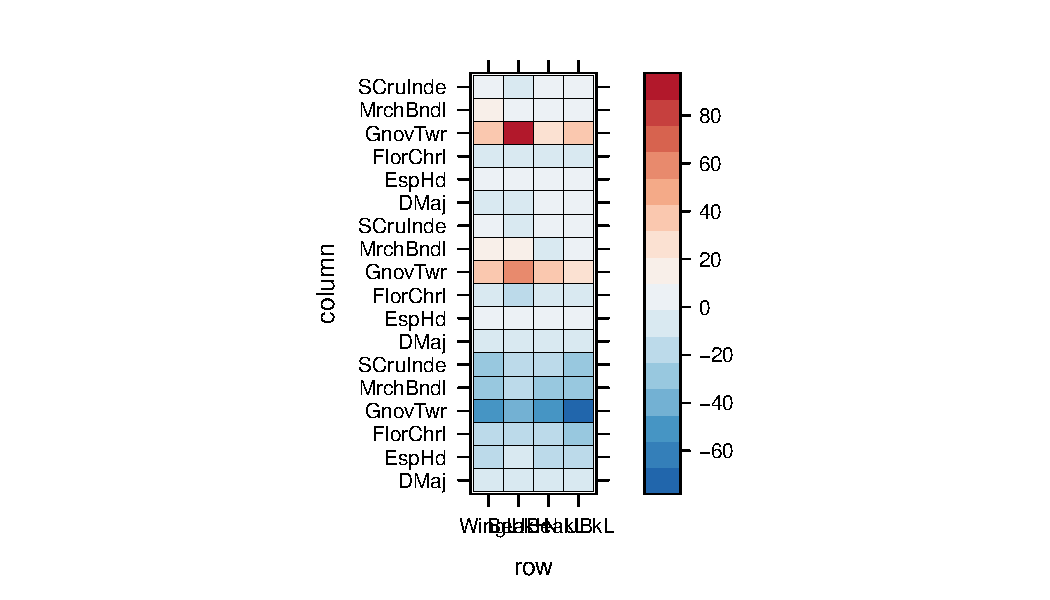
\includegraphics[width=\maxwidth]{figure/unnamed-chunk-65-2} 

\end{knitrout}

Compare metrics calculate on individual against metrics calculate after populationnal meaning
\begin{knitrout}
\definecolor{shadecolor}{rgb}{0.969, 0.969, 0.969}\color{fgcolor}\begin{kframe}
\begin{alltt}
\hlstd{ses.ind}\hlkwb{<-}\hlkwd{t}\hlstd{(}\hlkwd{rbind}\hlstd{(ses.list[[}\hlnum{1}\hlstd{]]}\hlopt{$}\hlstd{ses,}
      \hlstd{ses.list[[}\hlnum{2}\hlstd{]]}\hlopt{$}\hlstd{ses,}
      \hlstd{ses.list[[}\hlnum{3}\hlstd{]]}\hlopt{$}\hlstd{ses,}
      \hlstd{ses.list[[}\hlnum{4}\hlstd{]]}\hlopt{$}\hlstd{ses))}

\hlstd{ses.sp}\hlkwb{<-}\hlkwd{t}\hlstd{(}\hlkwd{rbind}\hlstd{(ses.list[[}\hlnum{5}\hlstd{]]}\hlopt{$}\hlstd{ses,}
     \hlstd{ses.list[[}\hlnum{6}\hlstd{]]}\hlopt{$}\hlstd{ses,}
     \hlstd{ses.list[[}\hlnum{7}\hlstd{]]}\hlopt{$}\hlstd{ses,}
     \hlstd{ses.list[[}\hlnum{8}\hlstd{]]}\hlopt{$}\hlstd{ses))}

\hlkwd{levelplot}\hlstd{(ses.ind,} \hlkwc{colorkey} \hlstd{= my.ckey,}
     \hlkwc{par.settings} \hlstd{= my.theme,}\hlkwc{border} \hlstd{=} \hlstr{"black"}\hlstd{)}
\end{alltt}
\end{kframe}
\includegraphics[width=\maxwidth]{figure/unnamed-chunk-66-1} 
\begin{kframe}\begin{alltt}
\hlkwd{levelplot}\hlstd{(ses.sp,} \hlkwc{colorkey} \hlstd{= my.ckey,}
     \hlkwc{par.settings} \hlstd{= my.theme,}\hlkwc{border} \hlstd{=} \hlstr{"black"}\hlstd{)}
\end{alltt}
\end{kframe}
\includegraphics[width=\maxwidth]{figure/unnamed-chunk-66-2} 

\end{knitrout}

\section{Multivariate analysis of metrics}
To finish, we can do a multivariate analysis of the metrics obtain during this tutorial using the package \texttt{ade4}. Analysis dudi 1 puts together all traits by meaning the SES values for each metrics in each sites whereas analysis dudi 2 analyses all combination of traits / sites / metrics.

\begin{knitrout}
\definecolor{shadecolor}{rgb}{0.969, 0.969, 0.969}\color{fgcolor}\begin{kframe}
\begin{alltt}
\hlkwd{library}\hlstd{(ade4)}

 \hlstd{matfordudi}\hlkwb{<-}\hlkwd{matrix}\hlstd{(}\hlkwc{nrow} \hlstd{=} \hlkwd{length}\hlstd{(}\hlkwd{colMeans}\hlstd{(ses.list[[}\hlnum{1}\hlstd{]]}\hlopt{$}\hlstd{ses)),} \hlkwc{ncol} \hlstd{=} \hlkwd{length}\hlstd{(}\hlkwd{names}\hlstd{(ses.list)))}
 \hlkwa{for}\hlstd{(i} \hlkwa{in} \hlnum{1}\hlopt{:} \hlkwd{length}\hlstd{(}\hlkwd{names}\hlstd{(ses.list)))\{}
  \hlstd{matfordudi[,i]}\hlkwb{<-}\hlkwd{colMeans}\hlstd{(ses.list[[i]]}\hlopt{$}\hlstd{ses)}
 \hlstd{\}}
 \hlkwd{colnames}\hlstd{(matfordudi)}\hlkwb{<-}\hlkwd{names}\hlstd{(ses.list)}
 \hlkwd{rownames}\hlstd{(matfordudi)}\hlkwb{<-}\hlkwd{colnames}\hlstd{(traits.finch)}

 \hlstd{matfordudi2}\hlkwb{<-}\hlkwd{matrix}\hlstd{(}\hlkwc{nrow} \hlstd{=} \hlkwd{length}\hlstd{(}\hlkwd{as.vector}\hlstd{(ses.list[[}\hlnum{1}\hlstd{]]}\hlopt{$}\hlstd{ses)),} \hlkwc{ncol} \hlstd{=} \hlkwd{length}\hlstd{(}\hlkwd{names}\hlstd{(ses.list)))}
 \hlkwa{for}\hlstd{(i} \hlkwa{in} \hlnum{1}\hlopt{:} \hlkwd{length}\hlstd{(}\hlkwd{names}\hlstd{(ses.list)))\{}
  \hlstd{matfordudi2[,i]}\hlkwb{<-}\hlkwd{as.vector}\hlstd{(ses.list[[i]]}\hlopt{$}\hlstd{ses)}
 \hlstd{\}}
 \hlkwd{colnames}\hlstd{(matfordudi2)}\hlkwb{<-}\hlkwd{names}\hlstd{(ses.list)}
\end{alltt}
\end{kframe}
\end{knitrout}

\begin{knitrout}
\definecolor{shadecolor}{rgb}{0.969, 0.969, 0.969}\color{fgcolor}\begin{kframe}
\begin{alltt}
\hlcom{#Use mice for the purpose of this example}
\hlstd{matfordudi}\hlkwb{<-}\hlkwd{complete}\hlstd{(}\hlkwd{mice}\hlstd{(matfordudi))}
\end{alltt}


{\ttfamily\noindent\bfseries\color{errorcolor}{\#\# Error in mice(matfordudi): No missing values found}}\begin{alltt}
\hlstd{matfordudi2}\hlkwb{<-}\hlkwd{complete}\hlstd{(}\hlkwd{mice}\hlstd{(matfordudi2))}
\end{alltt}


{\ttfamily\noindent\bfseries\color{errorcolor}{\#\# Error in mice(matfordudi2): No missing values found}}\end{kframe}
\end{knitrout}


\begin{knitrout}
\definecolor{shadecolor}{rgb}{0.969, 0.969, 0.969}\color{fgcolor}\begin{kframe}
\begin{alltt}
\hlstd{res.dudi}\hlkwb{<-}\hlkwd{dudi.pca}\hlstd{(}\hlkwd{t}\hlstd{(matfordudi),} \hlkwc{scan} \hlstd{= F,} \hlkwc{nf} \hlstd{=} \hlnum{2}\hlstd{)}
\hlkwd{s.corcircle}\hlstd{(res.dudi}\hlopt{$}\hlstd{co)}
\hlkwd{s.label}\hlstd{(res.dudi}\hlopt{$}\hlstd{li,} \hlkwc{add.plot} \hlstd{= T,} \hlkwc{clabel} \hlstd{=} \hlnum{0}\hlstd{,} \hlkwc{pch} \hlstd{=} \hlnum{16}\hlstd{)}
\hlkwd{s.label}\hlstd{(res.dudi}\hlopt{$}\hlstd{li}\hlopt{+}\hlnum{0.05}\hlstd{,} \hlkwc{add.plot} \hlstd{= T,} \hlkwc{boxes} \hlstd{= F)}
\end{alltt}
\end{kframe}
\includegraphics[width=\maxwidth]{figure/unnamed-chunk-69-1} 
\begin{kframe}\begin{alltt}
\hlstd{res.dudi2}\hlkwb{<-}\hlkwd{dudi.pca}\hlstd{(matfordudi2,} \hlkwc{scan} \hlstd{= F,} \hlkwc{nf} \hlstd{=} \hlnum{2}\hlstd{)}
\hlkwd{scatter}\hlstd{(res.dudi2)}
\end{alltt}
\end{kframe}
\includegraphics[width=\maxwidth]{figure/unnamed-chunk-69-2} 
\begin{kframe}\begin{alltt}
\hlkwd{s.corcircle}\hlstd{(res.dudi2}\hlopt{$}\hlstd{co)}
\end{alltt}
\end{kframe}
\includegraphics[width=\maxwidth]{figure/unnamed-chunk-69-3} 
\begin{kframe}\begin{alltt}
\hlkwd{s.class}\hlstd{(res.dudi2}\hlopt{$}\hlstd{li,} \hlkwd{as.factor}\hlstd{(}\hlkwd{c}\hlstd{(}\hlkwd{rep}\hlstd{(}\hlstr{"WingL"}\hlstd{,}\hlnum{6}\hlstd{),} \hlkwd{rep}\hlstd{(}\hlstr{"BeakH"}\hlstd{,}\hlnum{6}\hlstd{),}
                                  \hlkwd{rep}\hlstd{(}\hlstr{"UBeakL"}\hlstd{,}\hlnum{6}\hlstd{),} \hlkwd{rep}\hlstd{(}\hlstr{"N.UBkL"}\hlstd{,}\hlnum{6}\hlstd{))),}
        \hlkwc{col} \hlstd{=} \hlkwd{funky}\hlstd{(}\hlnum{4}\hlstd{))}
\end{alltt}
\end{kframe}
\includegraphics[width=\maxwidth]{figure/unnamed-chunk-69-4} 
\begin{kframe}\begin{alltt}
\hlkwd{s.class}\hlstd{(res.dudi2}\hlopt{$}\hlstd{li,} \hlkwd{as.factor}\hlstd{(}\hlkwd{rep}\hlstd{(}\hlkwd{c}\hlstd{(}\hlstr{"DMaj"}\hlstd{,}\hlstr{"EspHd"}\hlstd{,}\hlstr{"FlorChrl"}\hlstd{,}\hlstr{"GnovTwr"}\hlstd{,}
                                      \hlstr{"MrchBndl"}\hlstd{,}\hlstr{"SCruInde"}\hlstd{),}\hlnum{4} \hlstd{)),}
        \hlkwc{col} \hlstd{=} \hlkwd{funky}\hlstd{(}\hlnum{6}\hlstd{))}
\end{alltt}
\end{kframe}
\includegraphics[width=\maxwidth]{figure/unnamed-chunk-69-5} 

\end{knitrout}


\section{Speed of computation}

Speed of computation are saved throughout the vignette. For the specific system and R session describe above, we can determine the time of computation on darwin finch data with 99 permutations.

\begin{itemize}
\item \texttt{RaoRel} $->$ 0 s.
\item \texttt{decompCTRE} $->$ 0.14 s.
\item \texttt{partvar} $->$ 0.64 s.
\item \texttt{Tstats} $->$ 29.97 s.
\item \texttt{ComIndex} \begin{itemize}
    \item using four metrics $->$ 353.29 s.
    \item with/without intraspecific variation $->$ 199.59 s.
    \end{itemize}                    
\item \texttt{ComIndexMulti}: for the calcul of hv.3 see \pageref{hv.3} $->$ 202.52 s.
\end{itemize}

\begin{knitrout}
\definecolor{shadecolor}{rgb}{0.969, 0.969, 0.969}\color{fgcolor}\begin{kframe}
\begin{alltt}
\hlkwd{sessionInfo}\hlstd{()}
\end{alltt}
\begin{verbatim}
## R version 3.1.2 (2014-10-31)
## Platform: x86_64-w64-mingw32/x64 (64-bit)
## 
## locale:
## [1] LC_COLLATE=French_France.1252  LC_CTYPE=French_France.1252   
## [3] LC_MONETARY=French_France.1252 LC_NUMERIC=C                  
## [5] LC_TIME=French_France.1252    
## 
## attached base packages:
## [1] stats     graphics  grDevices utils     datasets  methods   base     
## 
## other attached packages:
##  [1] rasterVis_0.32      hexbin_1.27.0       latticeExtra_0.6-26
##  [4] RColorBrewer_1.1-2  raster_2.3-12       sp_1.0-16          
##  [7] geometry_0.3-5      magic_1.5-6         abind_1.4-0        
## [10] adegenet_1.4-2      hypervolume_1.1.1   rgl_0.95.1201      
## [13] mice_2.22           lattice_0.20-29     Rcpp_0.11.3        
## [16] cati_0.94           ape_3.2             ade4_1.6-2         
## [19] nlme_3.1-118        knitr_1.8          
## 
## loaded via a namespace (and not attached):
##  [1] class_7.3-11        colorspace_1.2-4    digest_0.6.8       
##  [4] e1071_1.6-4         evaluate_0.5.5      formatR_1.0        
##  [7] ggplot2_1.0.0       grid_3.1.2          gtable_0.1.2       
## [10] highr_0.4           htmltools_0.2.6     httpuv_1.3.2       
## [13] igraph_0.7.1        MASS_7.3-35         mime_0.2           
## [16] munsell_0.4.2       nnet_7.3-8          plyr_1.8.1         
## [19] proto_0.3-10        R6_2.0.1            randomForest_4.6-10
## [22] reshape2_1.4.1      RJSONIO_1.3-0       rpart_4.1-8        
## [25] scales_0.2.4        shiny_0.10.2.2      stringr_0.6.2      
## [28] tools_3.1.2         xtable_1.7-4        zoo_1.7-11
\end{verbatim}
\end{kframe}
\end{knitrout}

\begin{knitrout}
\definecolor{shadecolor}{rgb}{0.969, 0.969, 0.969}\color{fgcolor}\begin{kframe}
\begin{alltt}
\hlstd{proc.time_RaoRel}
\hlstd{proc.time_decompCTRE}
\hlstd{proc.time_partvar}
\hlstd{proc.time_Tstats}
\hlstd{proc.time_ComIndex1}
\hlstd{proc.time_ComIndex.with_without}
\hlstd{proc.time_ComIndexMulti}
\end{alltt}
\end{kframe}
\end{knitrout}


\section*{Conclusion}
\addcontentsline{toc}{subsection}{Conclusion}
This is the end of the tutorial. The up to date version of this tutorial is available \href{http://sourceforge.net/p/cati-r/code/ci/master/tree/tutorial/vignettes/vignette.pdf}{here}.

\section*{References}
\addcontentsline{toc}{subsection}{References}

\section*{Acknowledgment}
Great thanks to Thibault Jombart for his help on building R packages and writing tutorial with \href{http://yihui.name/knitr/}{knitR}.


\end{document}




ptm <- proc.time() 
proc.time_RaoRel <- proc.time() - ptm
